\section{Structural Elements for MTConnectDevices}
\label{sec:Structural Elements for MTConnectDevices}
\lstset{numbers=left,xleftmargin=2em}

\glspl{structural element} are \gls{xml} elements that form the logical structure for the \gls{mtconnectdevices} \gls{xml} document.  These elements are used to organize information that represents the physical and logical architecture of a piece of equipment.  Refer to \fig{mtconnect-devices-structural-elements} for an overview of the \glspl{structural element} used in an \gls{mtconnectdevices} document.

A variety of \glspl{structural element} are defined to describe a piece of equipment.  Some of these elements \MUST always appear in the \gls{mtconnectdevices} \gls{xml} document, while others are optional and \may be used, as required, to provide additional structure.

The first, or highest level, \gls{structural element} in a \gls{mtconnectdevices} \gls{xml} document is \gls{devices}. \gls{devices} is a container type \gls{xml} element used to group one or more pieces of equipment into a single \gls{xml} document.  \gls{devices} \MUST always appear in the \gls{mtconnectdevices} document.

\gls{device} is the next \gls{structural element} in the \gls{mtconnectdevices} \gls{xml} document. \gls{device} is also a container type \gls{xml} element. A separate \gls{device} container is used to identify each piece of equipment represented in the \gls{mtconnectdevices} document. Each \gls{device} container provides information on the physical and logical structure of the piece of equipment and the data associated with that equipment. \gls{device} can also represent any logical grouping of pieces of equipment that function as a unit or any other data source that provides data through an \gls{agent}.

One or more \gls{device} element(s) \MUST always appear in an \gls{mtconnectdevices} document.

\gls{components} is the next \gls{structural element} in the \gls{mtconnectdevices} \gls{xml} document. \gls{components} is also a container type XML element. \gls{components} is used to group information describing \gls{lower level} physical parts or logical functions of a piece of equipment.

If the \gls{components} container appears in the XML document, it \MUST contain one or more \gls{component} type XML elements.

\gls{component} is the next level of \gls{structural element} in the \gls{mtconnectdevices} \gls{xml} document. \gls{component} is both an abstract type \gls{xml} element and a container type element. 

As an abstract type element, \gls{component} will never appear in the \gls{xml} document describing a piece of equipment and will be replaced by a specific \gls{component} type defined in \sect{Component Structural Elements}. Each \gls{component} type is also a container type element. As a container, the \gls{component} type element is used to organize information describing \gls{lower level} \glspl{structural element} or \glspl{data entity} associated with the \gls{component}.

If \gls{lower level} \glspl{structural element} are described, these elements are by definition child \gls{component} elements of a parent \gls{component}. At this next level, the \gls{lower level} child \gls{component} elements are grouped into an \gls{xml} container called \gls{components}.
 
This \gls{lower level} \gls{components} container is comprised of one or more child \gls{component} \gls{xml} elements representing the sub-parts of the parent \gls{component}. Just like the parent \gls{component} element, the child \gls{component} element is an abstract type \gls{xml} element and will never appear in the \gls{xml} document – only the different \gls{lower level} child \gls{component} types will appear.

This parent-child relationship can continue to any depth required to fully define a piece of equipment.

\lst{component-levels} illustrates the relationship between a parent \gls{component} and \gls{lower level} child components:

\begin{lstlisting}[firstnumber=1,escapechar=|,%
    caption={Component Levels},label={lst:component-levels}]
<Devices>
  <Device>
    <Components>
      <Axes> | {\normalfont\it Parent Component} |
        <Components>
          <Rotary> | {\normalfont\it Child component of \gls{axes} and Parent component of \gls{lower level} components} |
            <Components>
              <Chuck> | {\normalfont\it Child Component of \gls{rotary}} |
\end{lstlisting}

\fig{mtconnect-devices-structural-elements} demonstrates the various \glspl{structural element} provided to describe a piece of equipment and the relationship between these elements.

\begin{figure}[ht]
  \centering
  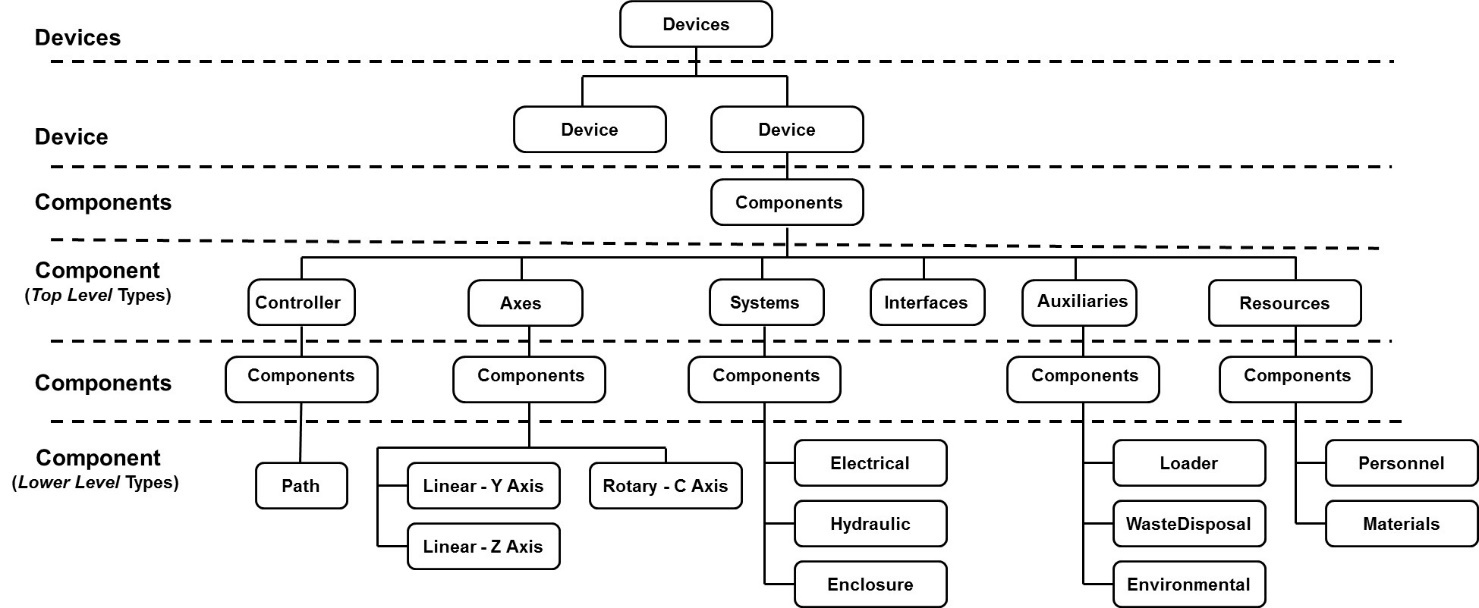
\includegraphics[width=0.95\textwidth]{figures/devices-structural-elements.png}
  \caption{Example Device Structural Elements}
  \label{fig:mtconnect-devices-structural-elements}
\end{figure}

\FloatBarrier

\gls{component} type \gls{xml} elements \may be further decomposed into \gls{composition} type \gls{xml} elements. \gls{composition} elements describe the lowest level basic structural or functional building blocks contained within a \gls{component}. Any number of \gls{composition} elements \may be used. Data provided for a \gls{component} provides more specific meaning when it is associated with one of the \gls{composition} elements of the \gls{component}.  The different \gls{composition} types that \may appear in the \gls{xml} document are defined in \sect{Composition Type Structural Elements}.

The \gls{composition} elements are organized into a \gls{compositions} container.  The \gls{compositions} container \may appear in the \gls{xml} document further describing a \gls{component}. If one or more \gls{composition} element(s) is provided to describe a \gls{component}, a \gls{compositions} container \MUST be defined for the \gls{component}.

\lst{component-levels-with-composition} represents an \gls{xml} document structure that demonstrates the relationship between a parent \gls{component} and its \gls{composition} elements.

\begin{lstlisting}[firstnumber=1,escapechar=|,%
    caption={Component levels with Composition},label={lst:component-levels-with-composition}]
<Devices>
  <Device>
    <Components>
      <Axes>  | {\normalfont\it (Component)} |
        <Components>
          <Linear> | {\normalfont\it (Component)} |
            <Compositions>
              <Composition>
              <Composition>
              <Composition>
\end{lstlisting}

\fig{composition-structural-elements} demonstrates this relationship between a \gls{component} and some of its potential \gls{composition} elements.

\begin{figure}[ht]
  \centering
  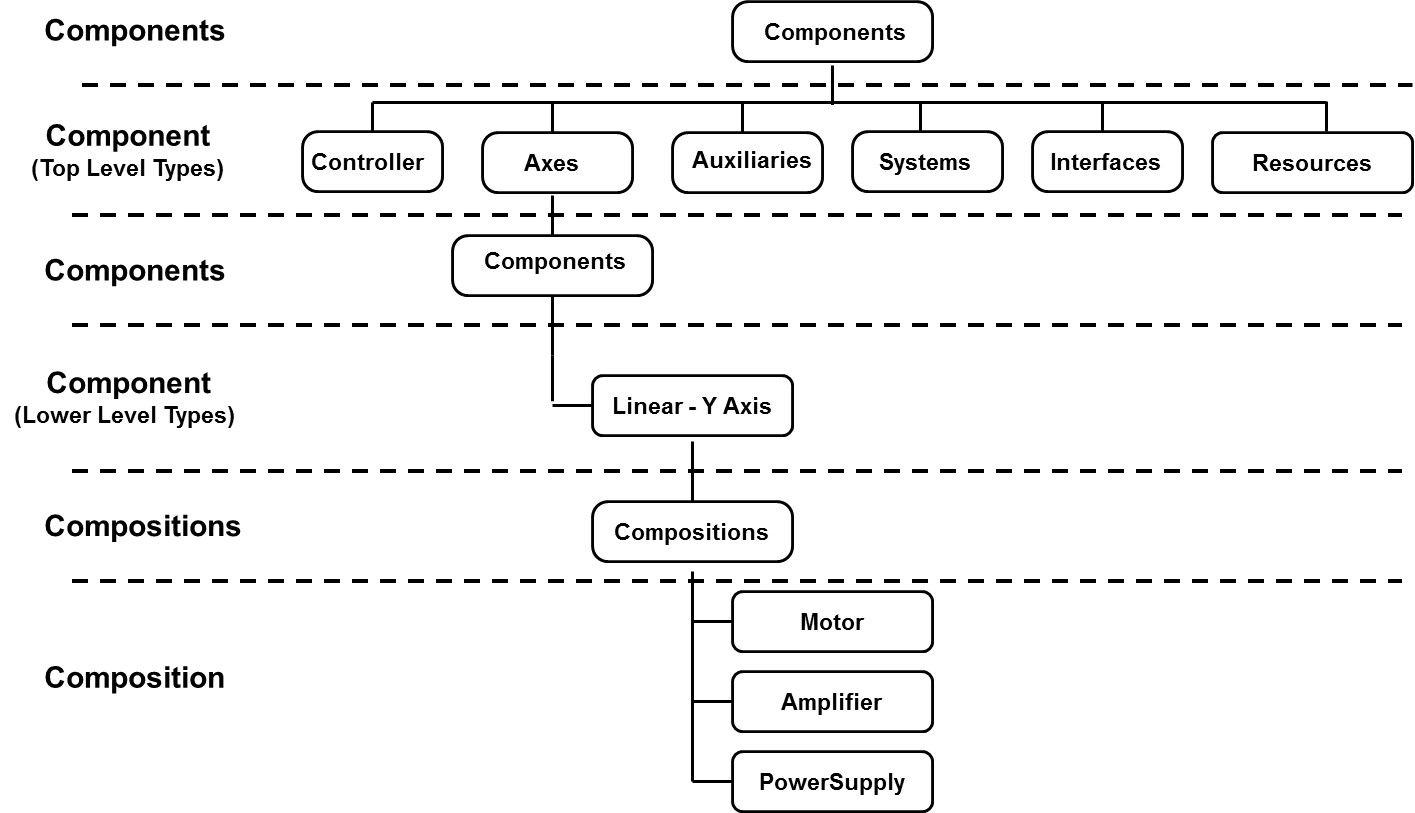
\includegraphics[width=.70\textwidth]{figures/composition-structural-elements.png}
  \caption{Example Composition Structural Elements}
  \label{fig:composition-structural-elements}
\end{figure}

\FloatBarrier

\subsection{Devices}
\label{sec:Devices}

\gls{devices} is a container type \gls{xml} element that \MUST contain only \gls{device} elements. \gls{devices} \MUST contain at least one \gls{device} element, but \may contain multiple \gls{device} elements.  \glspl{data entity} \MAYNOT be directly associated with the \gls{devices} container.

\tabulinesep = 5pt
\begin{longtabu} to \textwidth {
    |l|X[3l]|X[0.75l]|}
\caption{MTConnect Devices Element} \label{table:mtconnect-devices-element} \\

\hline
Element & Description & Occurrence \\
\hline
\endfirsthead

\hline
\multicolumn{3}{|c|}{Continuation of Table \ref{table:mtconnect-devices-element}}\\
\hline
Element & Description & Occurrence \\
\hline
\endhead
 
\gls{devices}	
&
The first, or highest level, \gls{structural element} in a \gls{mtconnectdevices} document. \gls{devices} is a container type XML element.
&
1 \\
\hline


\end{longtabu}

\pagebreak

\subsection{Device}

\gls{device} is an \gls{xml} container type element that organizes the \glspl{structural element} and \glspl{data entity} associated with a piece of equipment.  \glspl{data entity} \may be directly associated with the \gls{device} container.  \gls{device} \MUST provide the data item \gls{availability event}, which represents the \gls{agent}'s ability to communicate with the data source.

In the \gls{mtconnectdevices} \gls{xml} document, \gls{device} is a unique type of \gls{structural element}.  \gls{device} carries all of the properties of a \gls{component} (See \sect{Component}).  Additionally, \gls{device} \MUST have a \gls{uuid} attribute that uniquely identifies the piece of equipment.  The value for the \gls{uuid} \SHOULDNOT change over time.  The value for the \gls{uuid} \MUST be universally unique and \MUST only appear once in any MTConnect installation.  All \glspl{structural element} and \glspl{data entity} associated with a piece of equipment are therefore uniquely identified through their association with the \gls{device} container.

\tabulinesep = 5pt
\begin{longtabu} to \textwidth {
    |l|X[3l]|X[0.75l]|}
\caption{MTConnect Device Element} \label{table:mtconnect-device-element} \\

\hline
Element & Description & Occurrence \\
\hline
\endfirsthead

\hline
\multicolumn{3}{|c|}{Continuation of Table \ref{table:mtconnect-device-element}}\\
\hline
Element & Description & Occurrence \\
\hline
\endhead
 
\gls{device}	
&
\glsentrydesc{device} 
There \MAY be multiple \gls{device} elements in an XML document. 
&
1..* \\
\hline


\end{longtabu}


\begin{note}
Note: Some data sources may not be integral to a specific piece of equipment. These data sources may function independently or produce data that is not relevant to a specific piece of equipment. An example would be a temperature sensor installed in a plant to monitor the ambient air temperature. In such a case, these individual data sources, if they singularly or together perform a unique function, \may be modeled in a MTConnect XML document as a \gls{device}. When modeled as a \gls{device}, these data sources \must provide all of the data and capabilities defined for a device.

\end{note}

It is possible for a piece of equipment to be defined as both a \gls{component} of a \gls{device} and simultaneously function independently as a separate \gls{device} reporting data directly through an \gls{agent} using its own \gls{uuid}.  An example would be a temperature monitoring system that is defined as a \gls{device} reporting data about the environment within a facility and simultaneously reporting data for a \gls{component} of another piece of equipment that it is monitoring. 

\subsubsection{XML Schema Structure for Device}

\fig{device-schema-diagram} represents the structure of the \gls{device} XML element showing the attributes defined for \gls{device} and the elements that may be associated with \gls{device}.

\begin{figure}[ht]
  \centering
  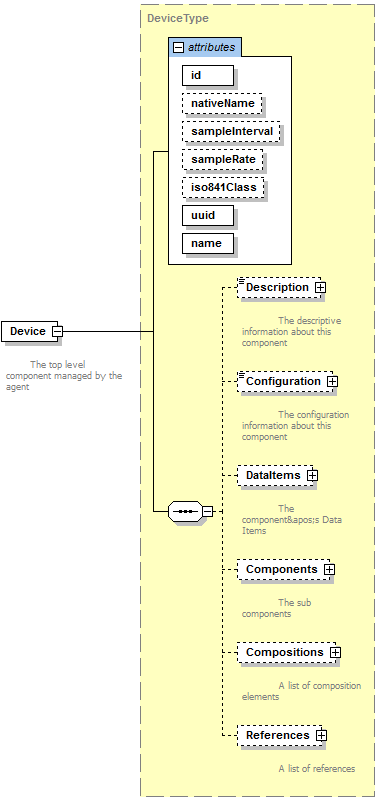
\includegraphics[width=.4\textwidth]{figures/device-schema-diagram.png}
  \caption{Device Diagram}
  \label{fig:device-schema-diagram}
\end{figure}

\FloatBarrier

\subsubsection{Attribute for Device}

\tbl{attributes-for-device} defines the attributes that may be used to provide additional information for a \gls{device} type element.

\tabulinesep = 5pt
\begin{longtabu} to \textwidth {
    |l|X[3l]|X[0.75l]|}
\caption{Attributes for Device} \label{table:attributes-for-device} \\

\hline
Attribute & Description & Occurrence \\
\hline
\endfirsthead

\hline
\multicolumn{3}{|c|}{Continuation of Table \ref{table:attributes-for-device}}\\
\hline
Attribute & Description & Occurrence \\
\hline
\endhead
 
\gls{id} 
&
\glsentrydesc{id}
\newline \gls{id} is a required attribute.
\newline An \gls{id} \MUST be unique across all the \gls{id} attributes in the document.
\newline An XML ID-type.
&
1 \\
\hline

\gls{nativename}
&
The common name normally associated with this piece of equipment.
\newline \gls{nativename} is an optional attribute. 
&
0..1 \\
\hline

\gls{sampleinterval} 
& 
An optional attribute that is an indication provided by a piece of equipment describing the interval in milliseconds between the completion of the reading of the data associated with the \gls{device} element until the beginning of the next sampling of that data. This indication is reported as the number of milliseconds between data captures.
\newline This information may be used by client software applications to understand how often information from a piece of equipment is expected to be refreshed.
\newline The refresh rate for all data from the piece of equipment will be the same as for the \gls{device} element unless specifically overridden by another \gls{sampleinterval} provided for a \gls{component} of the \gls{device} element.
\newline If the value of \gls{sampleinterval} is less than one millisecond, the value will be represented as a floating-point number. For example, an interval of 100 microseconds would be 0.1.
& 
0..1 \notesign \notesign \\
\hline

\deprecated{\gls{samplerate}}
&
\DEPRECATED in MTConnect Version 1.2. Replaced by \gls{sampleinterval}.
&
0..1 \notesign \notesign \notesign \\
\hline


\deprecated{\gls{iso841class}}
&
\DEPRECATED in MTConnect Version 1.1.
&
0..1 \notesign \notesign \notesign \\
\hline

\gls{uuid}
&
A unique identifier for this XML element.
\newline \gls{uuid} is a required attribute. 
\newline The uuid \MUST be unique amongst all uuid identifiers used in an MTConnect installation. 
\newline For example, this may be a combination of the manufacturer’s code and serial number. The \gls{uuid} \SHOULD be alphanumeric and not exceed 255 characters.
\newline An \gls{nmtoken} XML type.
&
1 \notesign \\
\hline

\gls{name}
&
The name of the piece of equipment represented by the \gls{device} element. 
\newline \gls{name} is a required attribute.
\newline This name \MUST be unique for each \gls{device} XML element defined in the \gls{mtconnectdevices} document.
\newline An \gls{nmtoken} XML type.
&
1 \\
\hline

\end{longtabu}


\begin{note}
Notes: \notesign A \gls{uuid} \MUST be provided for each \gls{device} element.  It is optional for all other \glspl{structural element}.\\ \notesign \notesign The \gls{sampleinterval} is used to aid a client software application in interpreting values provided by some \glspl{data entity}.  This is the desired sample interval and may vary depending on the capabilities of the piece of equipment.\\\notesign \notesign \notesign Remains in schema for backwards compatibility.

\end{note}

\subsubsection{Elements for Device}
\tbl{elements-for-device} lists the elements defined to provide additional information for a \gls{device} element. These elements are organized in the \gls{device} container.

\tabulinesep = 5pt
\begin{longtabu} to \textwidth {
    |l|X[3l]|X[0.75l]|}
\caption{Elements for Device} \label{table:elements-for-device} \\

\hline
Element & Description & Occurrence \\
\hline
\endfirsthead

\hline
\multicolumn{3}{|c|}{Continuation of Table \ref{table:elements-for-device}}\\
\hline
Element & Description & Occurrence \\
\hline
\endhead
 
\gls{description}
&
An XML element that can contain any descriptive content.
&
0..1 \\
\hline

\gls{configuration}
&
\glsentrydesc{configuration}
&
0..1 \\
\hline

\gls{dataitems}
&
A container for the \glspl{data entity} (See \sect{Data Entities for Device} and \sect{Listing of Data Items} for more detail) provided by this \gls{device} element.
&
1 \notesign \\
\hline

\gls{components}
&
A container for the \gls{component} elements associated with this \gls{device} element.
&
0..1 \\
\hline

\gls{compositions}
&
A container for the \gls{composition} elements associated with this \gls{device} element. 
&
0..1 \\
\hline

\gls{references}
&
A container for the \gls{reference} elements associated with this \gls{device} element.
&
0..1 \\
\hline

\end{longtabu}

\begin{note}
    Note: \notesign \gls{dataitems} \MUST be provided since every piece of equipment \MUST report \gls{availability event}.

\end{note}


\paragraph{Description for Device}\mbox{}

\fig{description-schema-diagram} shows the structure of the \gls{description} XML element showing the attributes defined for \gls{description}.  \gls{description} can contain any descriptive content for this piece of equipment.  This element is defined to contain mixed content and additional XML elements (indicated by the \gls{any} element) \may be added to extend the schema for \gls{description}.

\begin{figure}[ht]
  \centering
  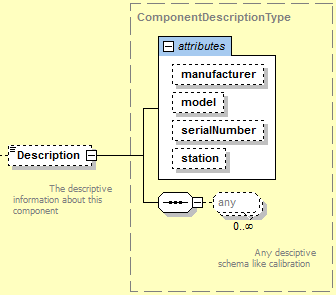
\includegraphics[width=.75\textwidth]{figures/description-schema-diagram.png}
  \caption{Description Diagram}
  \label{fig:description-schema-diagram}
\end{figure}

\FloatBarrier

\tbl{attributes-for-description} lists the attributes defined for the \gls{description} XML element.

\tabulinesep = 5pt
\begin{longtabu} to \textwidth {
    |l|X[3l]|X[0.75l]|}
\caption{Attributes for Description} \label{table:attributes-for-description} \\

\hline
Attribute & Description & Occurrence \\
\hline
\endfirsthead

\hline
\multicolumn{3}{|c|}{Continuation of Table \ref{table:attributes-for-description}}\\
\hline
Attribute & Description & Occurrence \\
\hline
\endhead

\gls{manufacturer}
&
The name of the manufacturer of the piece of equipment represented by the \gls{device} element. 
\newline \gls{manufacturer} is an optional attribute.
&
0..1 \\
\hline

\gls{model}
&
The model description of the piece of equipment represented by the \gls{device} element.
\newline \gls{model} is an optional attribute.
&
0..1 \\
\hline

\gls{serialnumber}
&
The serial number associated with piece of equipment represented by the \gls{device} element. 
\newline \gls{serialnumber} is an optional attribute.
&
0..1 \\
\hline

\gls{station}
&
The station where the equipment represented by the \gls{device} element is located when it is part of a manufacturing unit or cell with multiple stations. 
\newline \gls{station} is an optional attribute.
&
0..1 \\
\hline

\end{longtabu}

The content of \gls{description} \may include any additional descriptive information the implementer chooses to include regarding a piece of equipment.  This content \should be limited to information not included elsewhere in the \gls{mtconnectdevices} XML document.

\begin{lstlisting}[firstnumber=1,escapechar=|,%
    caption={Example of  Description},label={lst:example-of-description}]
<Description manufacturer="Example Co" 
    serialNumber="A124FFF" station="2"> Example Co 
    Simulated Vertical 3 Axis Machining center.
</Description>
\end{lstlisting}

\paragraph{Configuration for Device}\mbox{}
\label{sec:Configuration for Device}

The \gls{configuration} XML element contains technical information about a piece of equipment.  \gls{configuration} \MAY include any information describing the physical layout or functional characteristics of the piece of equipment, such as capabilities, testing, installation, operation, calibration, or maintenance. \gls{configuration} \MAY also include information representing the inter-relationships between pieces of equipment.

\tabulinesep = 5pt
\begin{longtabu} to \textwidth {
    |l|X[3l]|X[0.75l]|}
\caption{MTConnect Configuration Element} \label{table:mtconnect-configuration-element} \\

\hline
Element & Description & Occurrence \\
\hline
\endfirsthead

\hline
\multicolumn{3}{|c|}{Continuation of Table \ref{table:mtconnect-configuration-element}}\\
\hline
Element & Description & Occurrence \\
\hline
\endhead

\gls{configuration}
&
An XML element that contains technical information about a piece of equipment describing its physical layout, functional characteristics, and relationships with other pieces of equipment.
&
0..1 \\
\hline


\end{longtabu}

Configuration data for \gls{device} is structured in the \gls{mtconnectdevices} XML document as shown in \fig{configuration-diagram}.   \gls{abstractconfiguration} is an abstract type XML element.   It will never appear in the XML document representing a piece of equipment.    When \gls{configuration} is provided for a piece of equipment, that type of \gls{configuration} will appear in the XML document.

\gls{sensorconfiguration} is described in detail in \sect{Sensor Configuration}.

\gls{relationships} is described in detail in \sect{Relationships}.

\begin{figure}[ht]
  \centering
  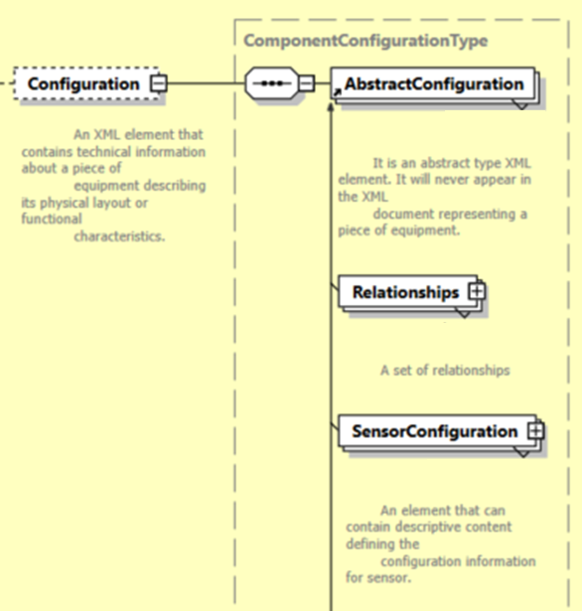
\includegraphics[width=0.7\textwidth]{figures/configuration-schema-diagram.png}
  \caption{Configuration Diagram}
  \label{fig:configuration-diagram}
\end{figure}
\FloatBarrier

\paragraph{DataItems for Device}\mbox{}

\gls{dataitems} is an \gls{xml} container that provides structure for organizing the data reported by a piece of equipment that is associated with the \gls{device} element.   

\gls{dataitems} \MUST be provided since every piece of equipment \MUST report the data item \gls{availability event}.

See \sect{Data Entities for Device} and \sect{Listing of Data Items} for details on the \gls{dataitems} \gls{xml} element.

\paragraph{Components within Device}\mbox{}

The use of the \gls{xml} container \gls{components} within a \gls{device} element provides the ability to break down the structure of a \gls{device} element into \gls{top level} and \gls{lower level} physical and logical sub-parts.  If a \gls{components} \gls{xml} element is provided, then only one \gls{components} element \MUST be defined for a \gls{device} element.

\paragraph{Compositions for Device}\mbox{}

\gls{compositions} is an \gls{xml} container used to organize \gls{composition} elements associated with a \gls{device} element.  See \sect{Compositions} for details on \gls{compositions}.

\paragraph{References for Device}\mbox{}

\gls{references} is an \gls{xml} container used to organize \gls{references} elements associated with a \gls{device} element.  See \sect{References} for details on \gls{references}.  

\subsection{Components}

\gls{components} is an \gls{xml} container used to group information describing physical parts or logical functions of a piece of equipment.   \gls{components} contains one or more \gls{component} \gls{xml} elements.

\tabulinesep = 5pt
\begin{longtabu} to \textwidth {
    |l|X[3l]|X[0.75l]|}
\caption{MTConnect Components Element} \label{table:mtconnect-components-element} \\

\hline
Element & Description & Occurrence \\
\hline
\endfirsthead

\hline
\multicolumn{3}{|c|}{Continuation of Table \ref{table:mtconnect-components-element}}\\
\hline
Element & Description & Occurrence \\
\hline
\endhead
 
\gls{components}
&
\glsentrydesc{components}
\newline If a \gls{components} XML element is provided, then only one \gls{components} element \MUST be defined for a \gls{device} element.
&
0..1 \\
\hline


\end{longtabu}

\subsection{Component}
\label{sec:Component}

A \gls{component} \gls{xml} element is a container type \gls{xml} element used to organize information describing a physical part or logical function of a piece of equipment.   It also provides structure for describing the \gls{lower level} \glspl{structural element} associated with the \gls{component}.     \gls{component} is an abstract type \gls{xml} element and will never appear directly in the MTConnect \gls{xml} document.  As an abstract type \gls{xml} element, \gls{component} will be replaced in the \gls{xml} document by specific \gls{component} types.  \gls{xml} elements representing \gls{component} are described in \sect{Component Structural Elements} and include elements such as \gls{axes}, \gls{controller}, and \gls{systems}.

\tabulinesep = 5pt
\begin{longtabu} to \textwidth {
    |l|X[3l]|X[0.75l]|}
\caption{MTConnect Component Element} \label{table:mtconnect-component-element} \\

\hline
Element & Description & Occurrence \\
\hline
\endfirsthead

\hline
\multicolumn{3}{|c|}{Continuation of Table \ref{table:mtconnect-component-element}}\\
\hline
Element & Description & Occurrence \\
\hline
\endhead
 
\gls{component}
&
\glsentrydesc{component}
\newline There can be multiple types of \gls{component} XML elements in the document.
&
1..* \\
\hline


\end{longtabu}

\subsubsection{XML Schema Structure for Component}
\label{sec:XML Schema Structure for Component}

\fig{component-schema-diagram} represents the structure of a \gls{component} \gls{xml} element showing the attributes defined for \gls{component} and the elements that \may be associated with \gls{component}.

\begin{figure}[ht]
  \centering
  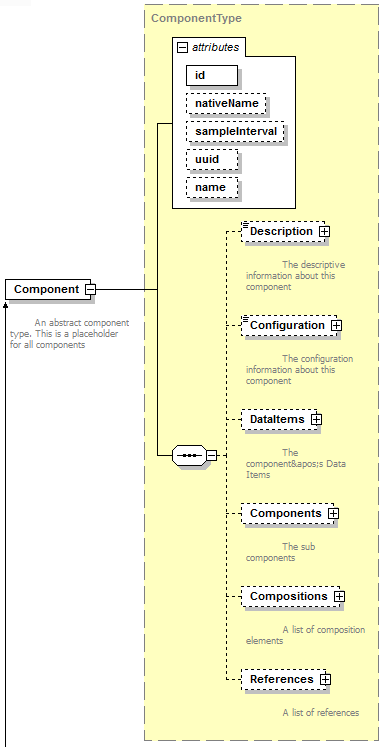
\includegraphics[width=.6\textwidth]{figures/component-schema-diagram.png}
  \caption{Component Diagram}
  \label{fig:component-schema-diagram}
\end{figure}

\FloatBarrier

\subsubsection{Attribute for Component}

\tbl{attributes-for-component} defines the attributes that may be used to provide additional information for a \gls{component} type \gls{xml} element.

\tabulinesep = 5pt
\begin{longtabu} to \textwidth {
    |l|X[3l]|X[0.75l]|}
\caption{Attributes for  Component} \label{table:attributes-for-component} \\

\hline
Attribute & Description & Occurrence \\
\hline
\endfirsthead

\hline
\multicolumn{3}{|c|}{Continuation of Table \ref{table:attributes-for-component}}\\
\hline
Attribute & Description & Occurrence \\
\hline
\endhead
 
\gls{id} 
&
\glsentrydesc{id}
\newline \gls{id} is a required attribute.
\newline An \gls{id} \MUST be unique across all the \gls{id} attributes in the document.
\newline An XML ID-type.
&
1 \\
\hline

\gls{nativename}
&
The common name normally associated with a specific physical or logical part of a piece of equipment.
\newline \gls{nativename} is an optional attribute. 
&
0..1 \\
\hline

\gls{sampleinterval}
&
An optional attribute that is an indication provided by a piece of
equipment describing the interval in milliseconds between the
completion of the reading of the data associated with the \gls{component} element until the beginning of the next sampling of that data. This indication is reported as the number of milliseconds between data captures.
\newline This information may be used by client software applications to understand how often information from a piece of equipment for a specific \gls{component} element is expected to be refreshed.
\newline The refresh rate for data from all \gls{lower level} \gls{component} elements will be the same as for the parent \gls{component} element unless specifically overridden by another \gls{sampleinterval} provided for the \gls{lower level} \gls{component} element.
\newline If the value of \gls{sampleinterval} is less than one millisecond, the value will be represented as a floating-point number. For example, an interval of 100 microseconds would be 0.1.
&
0..1 \notesign \notesign \\
\hline


\deprecated{\gls{samplerate}}
&
\DEPRECATED in MTConnect Version 1.2. Replaced by \gls{sampleinterval}.
&
0..1 \notesign \notesign \notesign \\
\hline

\gls{uuid}
&
A unique identifier for this XML element.
\newline \gls{uuid} is an optional attribute. 
\newline The value provided for the \gls{uuid} \MUST be unique amongst all \gls{uuid} identifiers used in an MTConnect installation. 
\newline For example, this may be a combination of the manufacturer’s code and serial number. The \gls{uuid} \SHOULD be alphanumeric and not exceed 255 characters.
\newline An \gls{nmtoken} XML type.
&
0..1 \notesign \\
\hline

\gls{name}
&
The name of the \gls{component} element.
\newline \gls{name} is an optional attribute.
\newline However, if there are multiple \gls{lower level} components that have the same parent and are of the same component type (example \gls{linear}), then the name attribute \MUST be provided for all \gls{lower level} components of the same element type to differentiate between the similar components.
\newline When provided, name \MUST be unique for all \gls{lower level} components of a parent \gls{component}.
\newline An \gls{nmtoken} XML type.
&
0..1 \\
\hline

\end{longtabu}

\begin{note}
Notes: \notesign While \gls{uuid} \must be provided for the \gls{device} element, it is optional for \gls{component} elements.\\\notesign \notesign The \gls{sampleinterval} is used to aid a client software application in interpreting values provided by some \glspl{data entity}.  This is the desired sample interval and may vary depending on the capabilities of the piece of equipment.\\\notesign \notesign \notesign Remains in schema for backwards compatibility.

\end{note}

\subsubsection{Elements of Component}

\tbl{elements-for-component} lists the elements defined to provide additional information for a \gls{component} type \gls{xml} element.

\tabulinesep = 5pt
\begin{longtabu} to \textwidth {
    |l|X[3l]|X[0.75l]|}
\caption{Elements for Component} \label{table:elements-for-component} \\

\hline
Element & Description & Occurrence \\
\hline
\endfirsthead

\hline
\multicolumn{3}{|c|}{Continuation of Table \ref{table:elements-for-component}}\\
\hline
Element & Description & Occurrence \\
\hline
\endhead
 
\gls{description}
&
An element that can contain any descriptive content.
&
0..1 \\
\hline

\gls{configuration}
&
\glsentrydesc{configuration}
&
0..1 \\
\hline

\gls{dataitems}
&
A container for the \glspl{data entity} (defined in \sect{Listing of Data Items}) associated with this \gls{component} element.
&
0..1 \notesign \\
\hline

\gls{components}
&
A container for \gls{lower level} \gls{component} XML elements associated with this parent \gls{component}.
&
0..1 \notesign \\
\hline

\gls{compositions}
&
A container for the \gls{composition} elements (defined in \sect{Composition Type Structural Elements}) associated with this \gls{component} element. 
&
0..1 \\
\hline

\gls{references}
&
A container for the \gls{reference} elements associated with this
\gls{component} element.
&
0..1 \notesign \\
\hline

\end{longtabu}

\begin{note}
    Note: \notesign At least one of \gls{components}, \gls{dataitems}, or \gls{references} \must be provided.

\end{note}

\paragraph{Description for Component}\mbox{}

\fig{description-of-component-schema-diagram} illustrates the structure of the \gls{description} \gls{xml} element showing the attributes defined for \gls{description}.  \gls{description} can contain any descriptive content of this \gls{component}.  This element is defined to contain mixed content and additional \gls{xml} elements (indicated by the \gls{any} element) \may be added to extend the schema for \gls{description}.

\begin{figure}[ht]
  \centering
  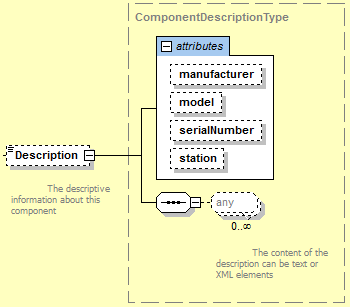
\includegraphics[width=.7\textwidth]{figures/description-of-component-schema-diagram.png}
  \caption{Description of Component Diagram}
  \label{fig:description-of-component-schema-diagram}
\end{figure}

\FloatBarrier

\tbl{attributes-for-component-description} lists the attributes defined for the \gls{description} \gls{xml} element.

\tabulinesep = 5pt
\begin{longtabu} to \textwidth {
    |l|X[3l]|X[0.75l]|}
\caption{Attributes for Description for Component} \label{table:attributes-for-component-description} \\

\hline
Attribute & Description & Occurrence \\
\hline
\endfirsthead

\hline
\multicolumn{3}{|c|}{Continuation of Table \ref{table:attributes-for-component-description}}\\
\hline
Attribute & Description & Occurrence \\
\hline
\endhead

\gls{manufacturer}
&
The name of the manufacturer of the physical or logical part of a piece of equipment represented by the \gls{component} element. 
\newline \gls{manufacturer} is an optional attribute.
&
0..1 \\
\hline

\gls{model}
&
The model description of the physical part or logical function of a piece of equipment represented by the \gls{component} element.
\newline \gls{model} is an optional attribute.
&
0..1 \\
\hline

\gls{serialnumber}
&
The serial number associated with the physical part or logical function of a piece of equipment represented by the \gls{component} element. 
\newline \gls{serialnumber} is an optional attribute.
&
0..1 \\
\hline

\gls{station}
&
The station where the physical part or logical function of a piece of equipment represented by the \gls{component} element is located when it is part of a manufacturing unit or cell with multiple stations. 
\newline \gls{station} is an optional attribute.
&
0..1 \\
\hline

\end{longtabu}

The content of \gls{description} \may include any additional descriptive information the implementer chooses to include regarding the \gls{component} element. This content \should be limited to information not included elsewhere in the \gls{mtconnectdevices} \gls{xml} document.  

\begin{lstlisting}[firstnumber=1,escapechar=|,%
    caption={Example of  Description},label={lst:example-of-description-for-component}]
<Description manufacturer="Example Co" 
    serialNumber="EXCO-TT-099PP-XXXX"> Advanced Pulse
    watt-hour transducer with pulse output
</Description>
\end{lstlisting}

\paragraph{Configuration for Component}\mbox{}
\label{sec:Configuration for Component}

The \gls{configuration} XML element contains technical information about a component.  \gls{configuration} \MAY include any information describing the physical layout or functional characteristics of a component, such as capabilities, testing, installation, operation, calibration, or maintenance. \gls{configuration} \MAY also include information representing the inter-relationships between components within a piece of equipment.

\tabulinesep = 5pt
\begin{longtabu} to \textwidth {
    |l|X[3l]|X[0.75l]|}
\caption{MTConnect Configuration Element for Component} \label{table:mtconnect-configuration-element-for-component} \\

\hline
Element & Description & Occurrence \\
\hline
\endfirsthead

\hline
\multicolumn{3}{|c|}{Continuation of Table \ref{table:mtconnect-configuration-element-for-component}}\\
\hline
Element & Description & Occurrence \\
\hline
\endhead

\gls{configuration}
&
An XML element that contains technical information about a component describing its physical layout, functional characteristics, and relationships with other components within a piece of equipment.
&
0..1 \\
\hline


\end{longtabu}

Configuration data for \gls{component} is structured in the \gls{mtconnectdevices} XML document as shown in \fig{component-configuration-diagram}.   \gls{abstractconfiguration} is an abstract type XML element.   It will never appear in the XML document representing a piece of equipment.    When \gls{configuration} is provided for a component, that type of \gls{configuration} will appear in the XML document.

\gls{sensorconfiguration} is described in detail in \sect{Sensor Configuration}.

\gls{relationships} is described in detail in \sect{Relationships}.

\begin{figure}[ht]
  \centering
  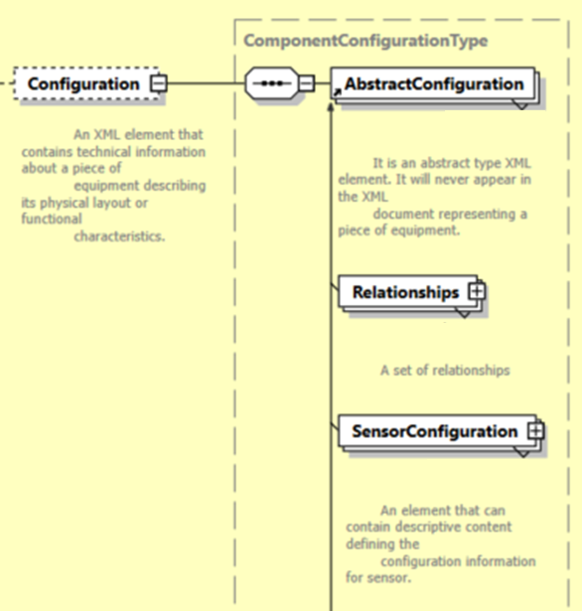
\includegraphics[width=0.6\textwidth]{figures/component-configuration-schema-diagram.png}
  \caption{Component Configuration Diagram}
  \label{fig:component-configuration-diagram}
\end{figure}
\FloatBarrier

\paragraph{DataItems for Component}\mbox{}

\gls{dataitems} is an \gls{xml} container that provides structure for organizing the data reported by a piece of equipment that is associated with the \gls{component}.   

See \sect{Data Entities for Device} for details on the \gls{dataitems} \gls{xml} element.

\newpage

\paragraph{Components within Component}\mbox{}

The use of the \gls{xml} container \gls{components} within a \gls{component} element provides the ability to further break down the structure of a \gls{component} element into even \gls{lower level} physical and logical sub-parts.  These \gls{lower level} elements can add more clarity and granularity to the physical or logical structure of a piece of equipment and the data associated with that equipment.

This parent-child relationship can be extended down to any level necessary to fully describe a piece of equipment. These \gls{lower level} \gls{component} elements use the same \gls{xml} structure as \gls{component} defined in \sect{XML Schema Structure for Component}.

\begin{lstlisting}[firstnumber=1,escapechar=|,%
    caption={Example of parent Component and Child Elements },label={lst:example-of-parent-component-and-child-elements}]
<Devices>
  <Device>
    <Components>
      <Axes> (Component)
        <Components>
          <Linear> (Component)
            <Components>
              <Etc. > (Component)
\end{lstlisting}

\paragraph{Compositions for Component}\mbox{}

\gls{compositions} is an \gls{xml} container used to organize the lowest level structural building blocks contained within a \gls{component} as defined below.

\paragraph{References for Component}\mbox{}

\gls{references} is an \gls{xml} container used to organize \gls{reference} elements associated with a \gls{component} element.  See \sect{References} for details on \gls{references}.

\subsection{Compositions}
\label{sec:Compositions}

\gls{compositions} is an \gls{xml} container that defines the lowest level structural building blocks contained within a \gls{component} element.   

\gls{compositions} contains one or more \gls{composition} \gls{xml} elements.

\tabulinesep = 5pt
\begin{longtabu} to \textwidth {
    |l|X[3l]|X[0.75l]|}
\caption{MTConnect Compositions Element} \label{table:mtconnect-compositions-element} \\

\hline
Element & Description & Occurrence \\
\hline
\endfirsthead

\hline
\multicolumn{3}{|c|}{Continuation of Table \ref{table:mtconnect-compositions-element}}\\
\hline
Element & Description & Occurrence \\
\hline
\endhead
 
\gls{compositions}
&
\glsentrydesc{compositions}
 Only one \gls{compositions} container \MAY appear for a \gls{component} element.
&
0..1 \\
\hline


\end{longtabu}

\subsection{Composition}

\gls{composition} \gls{xml} elements are used to describe the lowest level physical building blocks of a piece of equipment contained within a \gls{component}.

Like \gls{component} elements, \gls{composition} elements provide the ability to organize information describing \gls{lower level} sub-parts of a higher-level \gls{component} element.  However, unlike \gls{component}, \gls{composition} \mustnot be further sub-divided and \glspl{data entity} \mustnot be assigned to \gls{composition} elements.

\gls{composition} elements are used to add more clarity and granularity to the data being retrieved from a piece of equipment.  The meaning of the data associated with a \gls{component} may be enhanced by designating a specific \gls{composition} element associated with that data.  

An example of the additional detail provided when using \gls{composition} elements would be:

A \gls{temperature sample} associated with a \gls{linear} type axis may be further clarified by referencing the \gls{motor} or \gls{amplifier} type \gls{composition} element associated with that axis, which differentiates the temperature of the motor from the temperature of the amplifier.

\gls{composition} is a typed \gls{xml} element and will always define a specific type of structural building block contained within a \gls{component}.  \gls{xml} elements representing the types of \gls{composition} elements are described in \sect{Composition Type Structural Elements} and include elements describing such basic building blocks as motors, amplifiers, filters, and pumps.

\begin{lstlisting}[firstnumber=1,escapechar=|,%
    caption={Example of parent Component and child Composition elements} ,label={lst:example-of-parent-component-and-child-composition-elements}]
<Devices>
  <Device>
    <Components>
      <Axes> (Component)
        <Components>
          <Linear> (Component)
            <Compositions>
              <Composition>
              <Composition>
              <Composition>
\end{lstlisting}

\tabulinesep = 5pt
\begin{longtabu} to \textwidth {
    |l|X[3l]|X[0.75l]|}
\caption{MTConnect Composition Element} \label{table:mtconnect-composition-element} \\

\hline
Element & Description & Occurrence \\
\hline
\endfirsthead

\hline
\multicolumn{3}{|c|}{Continuation of Table \ref{table:mtconnect-composition-element}}\\
\hline
Element & Description & Occurrence \\
\hline
\endhead
 
\gls{composition}
&
\glsentrydesc{composition}
\newline \gls{composition} is a typed XML element.
\newline There can be multiple types of \gls{composition} XML elements defined for a \gls{component} element.
&
1..* \\
\hline


\end{longtabu}

\subsubsection{XML Schema Structure for Composition}

\fig{composition-schema-diagram} illustrates a \gls{composition} \gls{xml} element showing the attributes defined for \gls{composition} and the elements that may be associated with \gls{composition} type \gls{xml} elements.

\begin{figure}[ht]
  \centering
  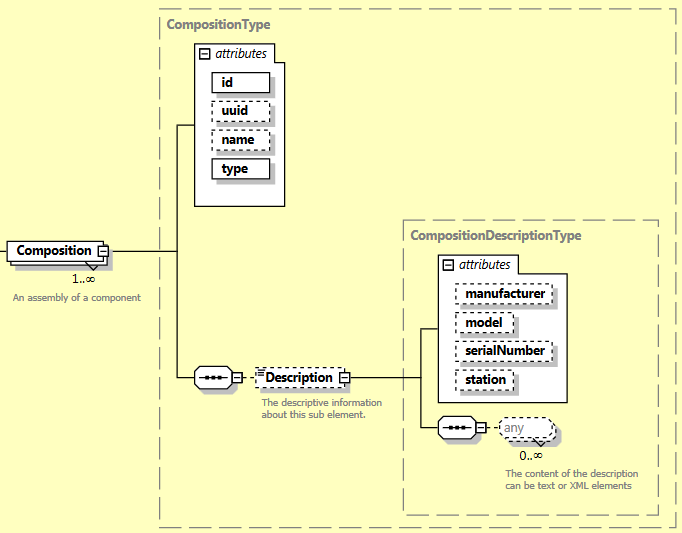
\includegraphics[width=.75\textwidth]{figures/composition-schema-diagram.png}
  \caption{Composition Diagram}
  \label{fig:composition-schema-diagram}
\end{figure}

\FloatBarrier

\subsubsection{Attributes for Composition}

\tbl{attributes-for-composition} defines the attributes that may be used to provide additional information for a \gls{composition} type \gls{xml} element.

\tabulinesep = 5pt
\begin{longtabu} to \textwidth {
    |l|X[3l]|X[0.75l]|}
\caption{Attributes for Composition} \label{table:attributes-for-composition} \\

\hline
Attribute & Description & Occurrence \\
\hline
\endfirsthead

\hline
\multicolumn{3}{|c|}{Continuation of Table \ref{table:attributes-for-composition}}\\
\hline
Attribute & Description & Occurrence \\
\hline
\endhead
 
\gls{id} 
&
\glsentrydesc{id}
\newline \gls{id} is a required attribute.
\newline An \gls{id} \MUST be unique across all the \gls{id} attributes in the document.
\newline An XML ID-type.
&
1 \\
\hline

\gls{uuid}
&
A unique identifier for this XML element.
\newline \gls{uuid} is an optional attribute. 
\newline The \gls{uuid} \MUST be unique amongst all \gls{uuid} identifiers used in an MTConnect installation. 
\newline For example, this may be a combination of the manufacturer’s code and serial number. The \gls{uuid} \SHOULD be alphanumeric and not exceed 255 characters.
\newline An \gls{nmtoken} XML type.
&
0..1 \\
\hline

\gls{name}
&
The name of the \gls{composition} element.
\newline \gls{name} is an optional attribute.
\newline If provided, \gls{name} \MUST be unique within a \gls{component} element.
\newline An \gls{nmtoken} XML type.
&
0..1 \\
\hline

\gls{type}
&
The type of \gls{composition} element.
\newline \gls{type} is a required attribute.
\newline Examples of types are \gls{motor}, \gls{filter type}, \gls{pump}, and \gls{amplifier}.
\newline Refer to \sect{Composition Type Structural Elements} for a list of currently defined types.
&
1 \\
\hline

\end{longtabu}

\subsubsection{Elements of Composition}

\tbl{elements-for-composition} lists the elements defined to provide additional information for a \gls{composition} type \gls{xml} element.

\tabulinesep = 5pt
\begin{longtabu} to \textwidth {
    |l|X[3l]|X[0.75l]|}
\caption{Elements for Composition} \label{table:elements-for-composition} \\

\hline
Element & Description & Occurrence \\
\hline
\endfirsthead

\hline
\multicolumn{3}{|c|}{Continuation of Table \ref{table:elements-for-composition}}\\
\hline
Element & Description & Occurrence \\
\hline
\endhead
 
\gls{description}
&
An element that can contain any descriptive content.
&
0..1 \\
\hline

\end{longtabu}

\paragraph{Description for Composition}\mbox{}

\fig{description-of-composition-schema-diagram} represents the structure of the \gls{description} \gls{xml} element showing the attributes defined for \gls{description}.  \gls{description} can contain any descriptive content for this \gls{composition} element.  This element is defined to contain mixed content and additional \gls{xml} elements (indicated by the \gls{any} element) \may be added to extend the schema for \gls{description}.

\begin{figure}[ht]
  \centering
  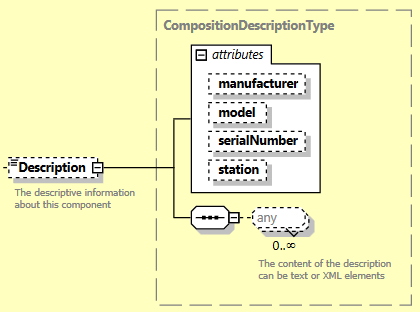
\includegraphics[width=.75\textwidth]{figures/description-of-composition-schema-diagram.png}
  \caption{Description of Composition Diagram}
  \label{fig:description-of-composition-schema-diagram}
\end{figure}

\FloatBarrier

\tbl{attributes-for-composition-description} lists the attributes defined for the \gls{description} \gls{xml} element. 

\tabulinesep = 5pt
\begin{longtabu} to \textwidth {
    |l|X[3l]|X[0.75l]|}
\caption{Attributes for Description for Composition} \label{table:attributes-for-composition-description} \\

\hline
Attribute & Description & Occurrence \\
\hline
\endfirsthead

\hline
\multicolumn{3}{|c|}{Continuation of Table \ref{table:attributes-for-composition-description}}\\
\hline
Attribute & Description & Occurrence \\
\hline
\endhead

\gls{manufacturer}
&
The name of the manufacturer of the physical part of a piece of equipment represented by the \gls{composition} element. 
\newline \gls{manufacturer} is an optional attribute.
&
0..1 \\
\hline

\gls{model}
&
The model description of the physical part of a piece of equipment represented by the \gls{composition} element.
\newline \gls{model} is an optional attribute.
&
0..1 \\
\hline

\gls{serialnumber}
&
The serial number associated with the physical part of a piece of equipment represented by the \gls{composition} element. 
\newline \gls{serialnumber} is an optional attribute.
&
0..1 \\
\hline

\gls{station}
&
The station where the physical part of a piece of equipment represented by the \gls{composition} element is located when it is part of a manufacturing unit or cell with multiple stations. 
\newline \gls{station} is an optional attribute.
&
0..1 \\
\hline

\end{longtabu}

The content of \gls{description} \may include any additional descriptive information the implementer chooses to include regarding the \gls{composition} element.  This content \should be limited to information not included elsewhere in the \gls{mtconnectdevices} \gls{xml} document.

\begin{lstlisting}[firstnumber=1,escapechar=|,%
    caption={Example of  Description},label={lst:example-of-description-for-composition}]
<Description manufacturer="Example Co" 
    serialNumber="A124FFF" station="2"> Spindle motor
    associated with Path 2.
</Description>
\end{lstlisting}

\subsection{References}
\label{sec:References}

\gls{references} is an \gls{xml} container that organizes pointers to information defined elsewhere within the \gls{xml} document for a piece of equipment.

\gls{references} may be modeled as part of a \gls{device}, \gls{component} or \gls{interface component} type \gls{structural element}.

\gls{references} contains one or more \gls{reference} \gls{xml} elements.

\tabulinesep = 5pt
\begin{longtabu} to \textwidth {
    |l|X[3l]|X[0.75l]|}
\caption{MTConnect References Element} \label{table:mtconnect-references-element} \\

\hline
Element & Description & Occurrence \\
\hline
\endfirsthead

\hline
\multicolumn{3}{|c|}{Continuation of Table \ref{table:mtconnect-references-element}}\\
\hline
Element & Description & Occurrence \\
\hline
\endhead
 
\gls{references}	
&
\glsentrydesc{references}
 Only one \gls{references} container \MUST appear for a \gls{device}, \gls{component}, or \gls{interface} element.
&
0..1 \\
\hline


\end{longtabu}

\subsection{Reference}

\gls{reference} is a pointer to information that is associated with another \gls{structural element} defined elsewhere in the \gls{xml} document for a piece of equipment.  That information may be data from the other element or the entire structure of that element.

\gls{reference} is an efficient method to associate information with an element without duplicating any of the data or structure.  For example, a Bar Feeder System may make a request for the \gls{barfeederinterface} and receive all the relevant data for the interface and the associated spindle (\gls{rotary} element) that is referenced as part of the \gls{barfeederinterface}.

\gls{reference} is an abstract type \gls{xml} element and will never appear directly in the MTConnect \gls{xml} document.  As an abstract type \gls{xml} element, \gls{reference} will be replaced in the \gls{xml} document by a specific \gls{reference} type.  The current supported types of \gls{reference} are \gls{dataitemref} and \gls{componentref} \gls{xml} elements.

\fig{reference-schema-diagram} represents the structure of the \gls{reference} \gls{xml} element.

\begin{figure}[ht]
  \centering
  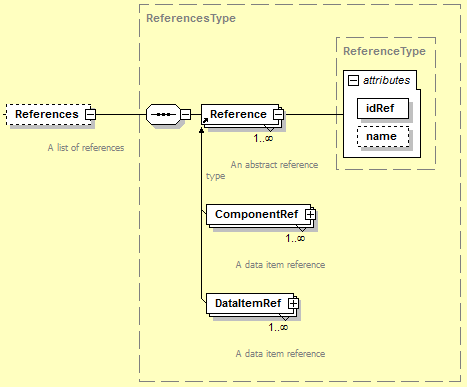
\includegraphics[width=.75\textwidth]{figures/reference-schema-diagram.png}
  \caption{Reference Diagram}
  \label{fig:reference-schema-diagram}
\end{figure}
\FloatBarrier

\subsubsection{ComponentRef}

\gls{componentref} \gls{xml} element is a pointer to all of the information associated with another \gls{structural element} defined elsewhere in the \gls{xml} document for a piece of equipment.  \gls{componentref} allows all of the information (\gls{lower level} \gls{components} and all \glspl{data entity}) that is associated with the other \gls{structural element} to be directly associated with this \gls{xml} element.

\fig{componentref-schema-diagram} represents the structure of a \gls{componentref} \gls{xml} element showing the attributes defined for \gls{componentref}.

\begin{figure}[ht]
  \centering
  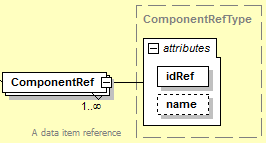
\includegraphics[width=.5\textwidth]{figures/componentref-schema-diagram.png}
  \caption{ComponentRef Diagram}
  \label{fig:componentref-schema-diagram}
\end{figure}

\FloatBarrier

\tbl{attributes-for-componentref} lists the attributes defined for the \gls{componentref} element. 

\tabulinesep = 5pt
\begin{longtabu} to \textwidth {
    |l|X[3l]|X[0.75l]|}
\caption{Attributes for ComponentRef} \label{table:attributes-for-componentref} \\

\hline
Attribute & Description & Occurrence \\
\hline
\endfirsthead

\hline
\multicolumn{3}{|c|}{Continuation of Table \ref{table:attributes-for-componentref}}\\
\hline
Attribute & Description & Occurrence \\
\hline
\endhead
 
\gls{idref} 
&
A pointer to the \gls{id} attribute of the \gls{component} that contains the information to be associated with this XML element.
\newline \gls{idref} is a required attribute.
&
1 \\
\hline

\gls{name}
&
The name of the \gls{componentref} element.
\newline \gls{name} is an optional attribute.
\newline However, if there are multiple \gls{componentref} elements defined for a \gls{component}, the \gls{name} attribute \MUST be provided for all \gls{componentref} elements to differentiate between the similar elements.
\newline When provided, \gls{name} \MUST be unique for all \gls{componentref} elements associated with the \gls{parent element}.
\newline An \gls{nmtoken} XML type.
&
0..1 \\
\hline

\end{longtabu}

\subsubsection{DataItemRef}

\gls{dataitemref} \gls{xml} element is a pointer to a \gls{data entity} associated with another \gls{structural element} defined elsewhere in the \gls{xml} document for a piece of equipment.  \gls{dataitemref} allows the data associated with a data item defined in another \gls{structural element} to be directly associated with this \gls{xml} element.

\fig{dataitemref-schema-diagram} represents the structure of a \gls{dataitemref} \gls{xml} element showing the attributes defined for \gls{dataitemref}.

\begin{figure}[ht]
  \centering
  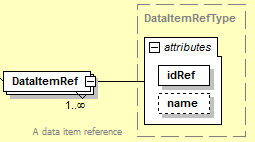
\includegraphics[width=.5\textwidth]{figures/dataitemref-schema-diagram.png}
  \caption{DataItemRef Diagram}
  \label{fig:dataitemref-schema-diagram}
\end{figure}

\FloatBarrier

\tbl{attributes-for-dataitemref} lists the attributes defined for the \gls{dataitemref} element. 

\tabulinesep = 5pt
\begin{longtabu} to \textwidth {
    |l|X[3l]|X[0.75l]|}
\caption{Attributes for DataItemRef} \label{table:attributes-for-dataitemref} \\

\hline
Attribute & Description & Occurrence \\
\hline
\endfirsthead

\hline
\multicolumn{3}{|c|}{Continuation of Table \ref{table:attributes-for-dataitemref}}\\
\hline
Attribute & Description & Occurrence \\
\hline
\endhead
 
\gls{idref} 
&
A pointer to the \gls{id} attribute of the \gls{dataitem} that contains the information to be associated with this XML element.
\newline \gls{idref} is a required attribute.
&
1 \\
\hline

\gls{name}
&
The name of the \gls{dataitemref} element.
\newline \gls{name} is an optional attribute.
\newline However, if there are multiple \gls{dataitemref} elements defined for a \gls{component}, the \gls{name} attribute \MUST be provided for all \gls{dataitemref} elements to differentiate between the similar elements.
\newline When provided, \gls{name} \MUST be unique for all \gls{dataitemref} elements associated with the \gls{parent element}.
\newline An \gls{nmtoken} XML type.
&
0..1 \\
\hline

\end{longtabu}

\newpage

\subsection{Relationships}
\label{sec:Relationships}

\gls{relationships} is an XML container that organizes information defining the association between pieces of equipment that function independently but together perform a manufacturing operation.  \gls{relationships} may also define the association between components within a piece of equipment.
 
\gls{relationships} may be modeled as part of a \gls{device} or a \gls{component} \gls{structural element}.
 
\gls{relationships} contains one or more \gls{relationship} XML elements.


\begin{longtabu} to \textwidth{|l|X[3l]|l|}
\caption{MTConnect Relationships Element} \label{table:mtconnect-relationships-element} \\

\hline
Element & Description & Occurrence \\
\hline
\endfirsthead

\hline
\multicolumn{3}{|c|}{Continuation of Table \ref{table:mtconnect-relationships-element}}\\
\hline
Element & Description & Occurrence \\
\hline
\endhead
 




\gls{relationships}
&
XML container consisting of one or more \gls{relationship} XML elements.
\newline Only one \gls{relationships} container \MUST appear for a \gls{device} or a \gls{component} element.
&
0..1 \\
\hline\end{longtabu}


\subsection{Relationship}
\label{sec:Relationship}

\gls{relationship} is an XML element that describes the association between two pieces of equipment that function independently but together perform a manufacturing operation. \gls{relationship} may also be used to define the association between two components within a piece of equipment.

\gls{relationship} is an abstract type XML element, \gls{relationship} will be replaced in the XML document by specific \gls{relationship} types.  XML elements representing \gls{relationship} are described in \sect{DeviceRelationship} and \sect{ComponentRelationship}.

A separate \gls{relationship} type element \MAY be defined to describe each pair of associations with a piece of equipment or between \gls{component} elements within a piece of equipment.

\newpage

Pieces of equipment may only be associated with other pieces of equipment and \gls{component} elements may only be associated with other \gls{component} elements within a specific piece of equipment.



The XML schema diagram in \fig{relationship-diagram} represents the structure of the \gls{relationship} XML element.

\begin{figure}[ht]
  \centering
  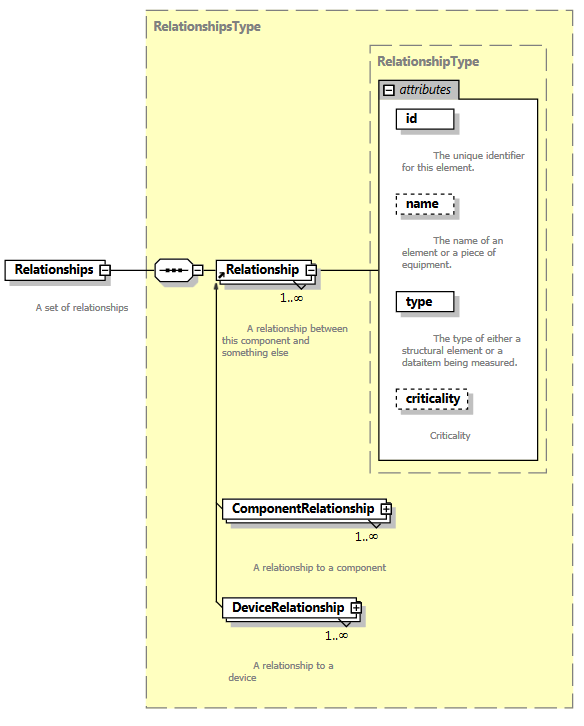
\includegraphics[width=0.8\textwidth]{figures/relationship-schema-diagram.png}
  \caption{Relationship Diagram}
  \label{fig:relationship-diagram}
\end{figure}
\FloatBarrier

\subsubsection{DeviceRelationship}
\label{sec:DeviceRelationship}

\gls{devicerelationship} describes the association between two pieces of equipment that function independently but together perform a manufacturing operation.

The XML schema diagram in \fig{devicerelationship-diagram} represents the structure of a \gls{devicerelationship} XML element showing the attributes defined for \gls{devicerelationship}.

\begin{figure}[ht]
  \centering
  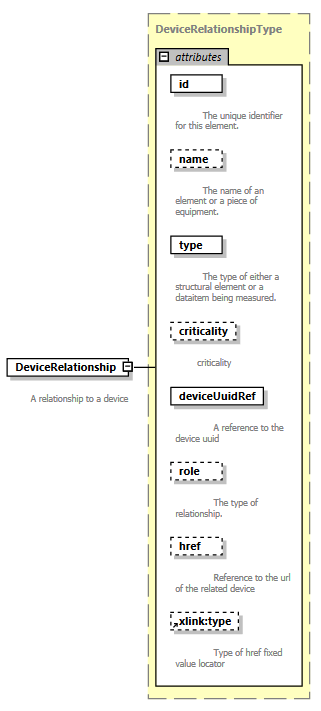
\includegraphics[width=0.6\textwidth]{figures/devicerelationship-schema-diagram.png}
  \caption{DeviceRelationship Diagram}
  \label{fig:devicerelationship-diagram}
\end{figure}
\FloatBarrier

The \tbl{attributes-for-devicerelationship} lists the attributes defined for the \gls{devicerelationship} element.


\begin{longtabu} to \textwidth{|l|X[3l]|l|}
\caption{Attributes for DeviceRelationship} \label{table:attributes-for-devicerelationship} \\

\hline
Attribute & Description & Occurrence \\
\hline
\endfirsthead

\hline
\multicolumn{3}{|c|}{Continuation of Table \ref{table:attributes-for-devicerelationship}}\\
\hline
Attribute & Description & Occurrence \\
\hline
\endhead
 




\gls{id}
&
The unique identifier for this \gls{devicerelationship}.
\newline \gls{id} is a required attribute.
\newline The \gls{id} attribute \MUST be unique within the \gls{mtconnectdevices} document.
\newline An XML ID-type.
&
1 \\
\hline

\gls{name}
&
The name associated with this \gls{devicerelationship}.
\newline \gls{name} is provided as an additional human readable identifier for this \gls{devicerelationship}.
\newline \gls{name} is an optional attribute.
\newline An \gls{nmtoken} XML type.
&
0..1 \\
\hline

\gls{type}
&
Defines the authority that this piece of equipment has relative to the associated piece of equipment.
\newline \gls{type} is a required attribute.
\newline The value provided for \gls{type} \MUST be one of the following values:
\newline \tab \gls{parent}:  This piece of equipment functions as a parent in the relationship with the associated piece of equipment.
\newline  \tab \gls{child}:  This piece of equipment functions as a child in the relationship with the associated piece of equipment.
\newline  \tab \gls{peer}:  This piece of equipment functions as a peer which provides equal functionality and capabilities in the relationship with the associated piece of equipment.
&
1 \\
\hline

\gls{criticality}
&
Defines whether the services or functions provided by the associated piece of equipment is required for the operation of this piece of equipment.
\newline \gls{criticality} is an optional attribute.
\newline The value provided for \gls{criticality} \MUST be one of the following values:
\newline \tab \gls{critical}:  The services or functions provided by the associated piece of equipment is required for the operation of this piece of equipment.
\newline  \tab \gls{noncritical}:  The services or functions provided by the associated piece of equipment is not required for the operation of this piece of equipment.
&
0..1 \\
\hline

\gls{deviceuuidref}
&
A reference to the associated piece of equipment.
\newline The value provided for \gls{deviceuuidref} \MUST be the value provided for the \gls{uuid} attribute of the \gls{device} element of the associated piece of equipment.
\newline \gls{deviceuuidref} is a required attribute.
\newline An \gls{nmtoken} XML type.
&
1 \\
\hline

\gls{role}
&
Defines the services or capabilities that the referenced piece of equipment provides relative to this piece of equipment.
\newline \gls{role} is an optional attribute.
\newline The value provided for \gls{role} \MUST be one of the following values:
\newline  \tab \gls{system condition}:  The associated piece of equipment performs the functions of a \cfont{System} for this piece of equipment.  In MTConnect, \cfont{System} provides utility type services to support the operation of a piece of equipment and these services are required for the operation of a piece of equipment.
\newline  \tab \gls{auxiliary subtype}:  The associated piece of equipment performs the functions as an \cfont{Auxiliary} for this piece of equipment.  In MTConnect, \cfont{Auxiliary} extends the capabilities of a piece of equipment, but is not required for the equipment to function.
&
0..1 \\
\hline

\gls{href}
&
A URI identifying the \gls{agent} that is publishing information for the associated piece of equipment. \gls{href} \MUST also include the UUID for that specific piece of equipment.
\newline \gls{href} is of type \cfont{xlink:href} from the W3C XLink specification: (https://www.w3.org/TR/xlink11/).
\newline \gls{href} is an optional attribute.
&
0..1 \\
\hline

\gls{xlink:type}
&
The XLink \cfont{type} attribute \MUST have a fixed value of \cfont{locator} as defined in W3C XLink 1.1 https://www.w3.org/TR/xlink11/ \textit{section 5.4 Locator Attribute (\gls{href})}.
\newline If the \gls{href} attribute is provided, it \MUST conform to the URI syntactic rules as defined in IETF RFC 3986 for Uniform Resource Identifiers. (https://www.ietf.org/rfc/rfc3986.txt)
&
0..1 \\\hline
\hline\end{longtabu}



\subsubsection{ComponentRelationship}
\label{sec:ComponentRelationship}

\gls{componentrelationship} describes the association between two components within a piece of equipment that function independently but together perform a capability or service within a piece of equipment.

The XML schema in \fig{componentrelationship-diagram} represents the structure of a \gls{componentrelationship} XML element showing the attributes defined for \gls{componentrelationship}.

\begin{figure}[ht]
  \centering
  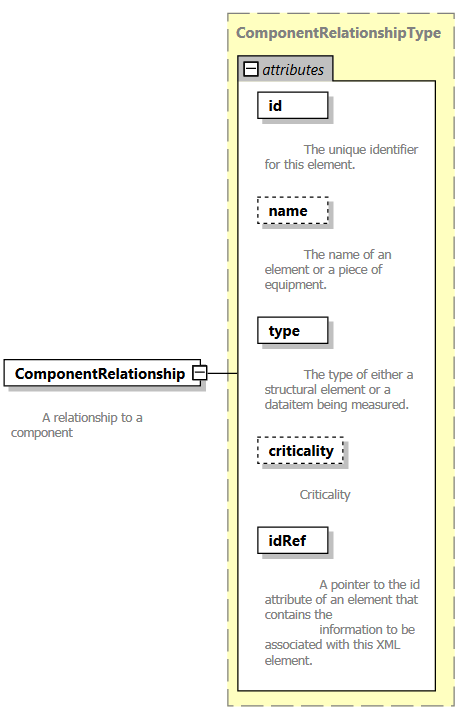
\includegraphics[width=0.6\textwidth]{figures/componentrelationship-schema-diagram.png}
  \caption{ComponentRelationship Diagram}
  \label{fig:componentrelationship-diagram}
\end{figure}
\FloatBarrier

The \tbl{attributes-for-componentrelationship} lists the attributes defined for the \gls{componentrelationship} element.


\begin{longtabu} to \textwidth{|l|X[3l]|l|}
\caption{Attributes for ComponentRelationship} \label{table:attributes-for-componentrelationship} \\

\hline
Attribute & Description & Occurrence \\
\hline
\endfirsthead

\hline
\multicolumn{3}{|c|}{Continuation of Table \ref{table:attributes-for-componentrelationship}}\\
\hline
Attribute & Description & Occurrence \\
\hline
\endhead
 




\gls{id}
&
The unique identifier for this \gls{componentrelationship}.
\newline \gls{id} is a required attribute.
\newline The \gls{id} attribute \MUST be unique within the \gls{mtconnectdevices} document.
\newline An XML ID-type.
&
1 \\
\hline

\gls{name}
&
The name associated with this \gls{componentrelationship}.
\newline \gls{name} is provided as an additional human readable identifier for this \gls{componentrelationship}.
\newline \gls{name} is an optional attribute.
\newline An \gls{nmtoken} XML type.
&
0..1 \\
\hline

\gls{type}
&
Defines the authority that this component element has relative to the associated component element.
\newline \gls{type} is a required attribute.
\newline The value provided for \gls{type} \MUST be one of the following values:
\newline \tab \gls{parent}:  This component functions as a parent in the relationship with the associated component element.
\newline  \tab \gls{child}:  This component functions as a child in the relationship with the associated component element.
\newline  \tab \gls{peer}:  This component functions as a peer which provides equal functionality and capabilities in the relationship with the associated component element.
&
1 \\
\hline

\gls{criticality}
&
Defines whether the services or functions provided by the associated component element is required for the operation of this piece of equipment.
\newline \gls{criticality} is an optional attribute.
\newline The value provided for \gls{criticality} \MUST be one of the following values:
\newline \tab \gls{critical}:  The services or functions provided by the associated component element is required for the operation of this piece of equipment.
\newline  \tab \gls{noncritical}:  The services or functions provided by the associated component element is not required for the operation of this piece of equipment.
&
0..1 \\
\hline

\gls{idref}
&
A reference to the associated component element.
\newline The value provided for \gls{idref} \MUST be the value provided for the \gls{id} attribute of the associated \gls{component} element.
\newline \gls{idref} is a required attribute.
\newline An \gls{nmtoken} XML type.
&
1 \\
\hline\end{longtabu}

\section{Component Structural Elements}
\label{sec:Component Structural Elements}

\gls{component} \glspl{structural element} are \gls{xml} containers used to represent physical parts or logical functions of a piece of equipment.

\gls{component} \glspl{structural element} are defined into two major categories:

\begin{itemize}

\item \gls{top level} \gls{component} elements are used to group the \glspl{structural element} representing the most significant physical or logical functions of a piece of equipment.  The \gls{top level} \gls{component} elements provided in an \gls{mtconnectdevices} document \should be restricted to those defined in \tbl{elements-toplevel-for-component}.  However, these \gls{top level} \gls{component} elements \may also be used as \gls{lower level} \gls{component} elements; as required.

\item \gls{lower level} \gls{component} elements are used to describe the sub-parts of the parent \gls{component} to provide more clarity and granularity to the physical or logical structure of the \gls{top level} \gls{component} elements.
\end{itemize}

This section of the \glspl{device information model} provides guidance for the most common relationships between \gls{top level} \gls{component} elements and \gls{lower level} child components.  However, all \gls{component} elements \may be used in any configuration, as required, to fully describe a piece of equipment.

As described in \sect{Structural Elements for MTConnectDevices}, \gls{component} is an abstract type \gls{structural element} within the \glspl{device information model} and will never appear directly in the \gls{mtconnectdevices} \gls{xml} document.  As abstract type \gls{xml} elements, \gls{component} will be replaced in the \gls{xml} document by a specific \gls{component} type.

\tbl{elements-toplevel-for-component} defines the \gls{top level} \gls{component} elements available to describe a piece of equipment.

\tabulinesep = 5pt
\begin{longtabu} to \textwidth {
    |l|X[3l]|}
\caption{Top Level Component Elements} \label{table:elements-toplevel-for-component} \\

\hline
Top Level Component Element \notesign \notesign & Description\\
\hline
\endfirsthead

\hline
\multicolumn{2}{|c|}{Continuation of Table \ref{table:elements-toplevel-for-component}}\\
\hline
Top Level Component Element \notesign \notesign & Description\\
\hline
\endhead
 
\gls{axes}	
&
\glsentrydesc{axes} \\
\hline

\gls{controller}
&
\glsentrydesc{controller}
\\
\hline

\gls{systems}
&
\glsentrydesc{systems} \\
\hline

\gls{auxiliaries}
&
\glsentrydesc{auxiliaries} \\
\hline

\gls{resources}	
&
\glsentrydesc{resources} \\
\hline

\gls{interfaces component}	
&
\glsentrydesc{interfaces component} \\
\hline

\end{longtabu}


\begin{note}
Note: \notesign \notesign The following components have been relocated or redefined since they are not classified as restricted \gls{top level} components:\\- \gls{power} was \DEPRECATED in MTConnect Version 1.1 and was replaced by the \gls{data entity} called \gls{availability event}.\\- \gls{door component} has been redefined as a \gls{lower level} component of a parent \gls{component} element or as a \gls{composition} element.\\- \gls{actuator}, due to its uniqueness, has been redefined as a piece of equipment with the ability to be represented as a \gls{lower level} component of a parent \gls{component} element or as a \gls{composition} element.\\- \gls{sensor}, due to its uniqueness, has been redefined as a piece of equipment with the ability to be represented as a \gls{lower level} component of a parent \gls{component} element (See \sect{Sensors} for further detail).\\ - \gls{stock} has been redefined as a \gls{lower level} component of the \gls{resources} \gls{top level} \gls{component} element.

\end{note}

The common relationship between the \gls{top level} \gls{component} elements and the \gls{lower level} child \gls{component} elements are described below.  It should be noted that as the MTConnect Standard evolves, more \gls{component} types will be added to organize information for new types of equipment and/or new physical or logical sub-parts of equipment. 

\subsection{Axes}

\gls{axes} is a \gls{top level} \gls{component} element.  It is a container that organizes information representing the \glspl{structural element} that perform linear or rotational motion for a piece of equipment.

\gls{axes} organizes information for the individual physical axes into \gls{component} types of \gls{linear} and \gls{rotary} based on the type of motion performed by each axis.  \gls{axes} \must contain at least one \gls{linear} or one \gls{rotary} type axis.

\fig{axes-example-two-linear-one-rotary} defines the relationship between the \gls{axes} container and the individual axis type \glspl{structural element}.

\begin{figure}[ht]
  \centering
  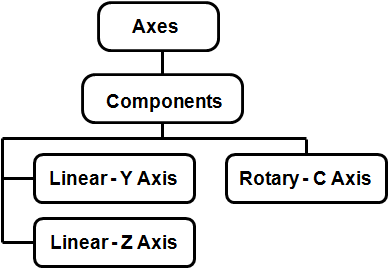
\includegraphics[width=.5\textwidth]{figures/axes-example-two-linear-one-rotary.png}
  \caption{Axes Example with Two Linear Axes and One Rotary Axis}
  \label{fig:axes-example-two-linear-one-rotary}
\end{figure}

\FloatBarrier

\subsubsection{Linear}

A \gls{linear} axis represents the movement of a physical piece of equipment, or a portion of the equipment, in a straight line.

Movement may be either in a positive or negative direction.

\gls{linear} type axes \must be identified using a value for the name attribute as X, Y, or Z with numbers appended for additional axes in the same plane.  Additional linear axes are often referred to as U, V, and W.   However, MTConnect defines the secondary axes to X, Y, and Z as X2, Y2, and Z2.

If the piece of equipment is unable to provide information associated with the \gls{name} attribute, then the \gls{nativename} attribute \must be included to identify the axis.

\subsubsection{Rotary}

A \gls{rotary} axis represents any non-linear or rotary movement of a physical piece of equipment or a portion of the equipment.

\gls{rotary} type axes \must be identified using a value for the \gls{name} attribute as A, B, and C for axes that rotate around the X, Y, and Z axes respectively.  As with the \gls{linear} axes, a number \must be appended for additional axes in the same plane (C, C2, C3, C4, ...).

If the piece of equipment is unable to provide information associated with the \gls{name} attribute, then the \gls{nativename} attribute \must be included to identify the axis.

An axis whose function is to provide rotary motion may function as a continuous rotation (\gls{spindle value} mode), continuous-path contour rotary motion (\gls{contour value} mode), or positioning (\gls{index value} mode) to discrete rotary positions.   As such, a \gls{rotary} type axis \should specify a \gls{rotarymode event} data item identifying the operating mode of the axis: \gls{spindle value}, \gls{index value}, or \gls{contour value}.

\paragraph{Chuck}\mbox{}

\gls{chuck component} is an \gls{xml} container that provides the information about a mechanism that holds a part or stock material in place.   It may also represent the information about any other type mechanism that holds items in place within a piece of equipment.

The operation of a \gls{chuck component} when represented as a \gls{component} element is defined by \gls{chuckstate event}. The value of \gls{chuckstate event} \must be \gls{open value}, \gls{closed value}, or \gls{unlatched value}.

\gls{chuck component} may be used in the \gls{mtconnectdevices} document as either a \gls{lower level} component or as a \gls{composition} element of a parent \gls{component} element.

\subsection{Controller}

\gls{controller} is a \gls{top level} container that organizes information for an intelligent part of a piece of equipment that monitors and calculates information to alter the operating conditions of the equipment.  Typical types of controllers for a piece of equipment include CNC (Computer Numerical Control), PAC (Programmable Automation Control), IPC (Industrialized Computer), or IC (Imbedded Computer).

\gls{controller} is a component that organizes and provides information regarding the execution of a control program(s), the mode of operation of the piece of equipment, and fault information regarding the operation of the equipment.

\begin{note}
Note: MTConnect Version 1.1.0 and later implementations \should use a \gls{lower level} \gls{component} element called \gls{path} to represent an individual tool path or other independent function within a \gls{controller} element.  When the \gls{controller} element is capable of executing more than one simultaneous and independent programs, the implementation \must specify a \gls{lower level} \gls{path} element representing each of the independent functions of the \gls{controller}.

\end{note}

\subsubsection{Path}

\gls{path} is an \gls{xml} container that represents the information for an independent operation or function within a \gls{controller}.  For many types of equipment, \gls{path} represents a set of \gls{axes}, one or more Program elements, and the data associated with the motion of a control point as it moves through space.   However, it \may also represent any independent function within a \gls{controller} that has unique data associated with that function.

\gls{path} \should provide an \gls{execution event} data item to define the operational state of the \gls{controller} component of the piece of equipment.

If the \gls{controller} is capable of performing more than one independent operation or function simultaneously, a separate \gls{path} component \must be used to organize the data associated with each independent operation or function.

\subsection{Systems}

\gls{systems} is a \gls{top level} \gls{xml} container that provides structure for the information describing one or more \gls{lower level} functional systems that perform as discrete operating modules of the equipment or provide utility type services to support the operation of the equipment. These systems are required for the piece of equipment to perform its intended function and are permanently integrated into the piece of equipment.

Since these systems operate as separate functional units, they are represented in the \gls{mtconnectdevices} \gls{xml} document as individual \gls{lower level} \gls{component} elements of \gls{systems} based on the function or service provided. 

\subsubsection{Hydraulic System}

\gls{hydraulic} is an \gls{xml} container that represents the information for a system comprised of all the parts involved in moving and distributing pressurized liquid throughout the piece of equipment.

\subsubsection{Pneumatic System}

\gls{pneumatic} is an \gls{xml} container that represents the information for a system comprised of all the parts involved in moving and distributing pressurized gas throughout the piece of equipment. 

\subsubsection{Coolant System}

\gls{coolant} is an \gls{xml} container that represents the information for a system comprised of all the parts involved in distribution and management of fluids that remove heat from a piece of equipment.

\subsubsection{Lubrication System}

\gls{lubrication} is an \gls{xml} container that represents the information for a system comprised of all the parts involved in distribution and management of fluids used to lubricate portions of the piece of equipment.

\subsubsection{Electric System}

\gls{electric} is an \gls{xml} container that represents the information for the main power supply for device piece of equipment and the distribution of that power throughout the equipment.  The electric system will provide all the data with regard to electric current, voltage, frequency, etc. that applies to the piece of equipment as a functional unit.   Data regarding electric power that is specific to a \gls{component} will be reported as \glspl{data entity} for that specific \gls{component}.

\subsubsection{Enclosure System}

\gls{enclosure} is an \gls{xml} container that represents the information for a structure used to contain or isolate a piece of equipment or area.  The \gls{enclosure} system may provide information regarding access to the internal components of a piece of equipment or the conditions within the enclosure.   For example, \gls{door component} may be defined as a \gls{lower level} \gls{component} or \gls{composition} element of the \gls{enclosure} system.

\subsubsection{Protective System}

\gls{protective} is an \gls{xml} container that represents the information for those functions that detect or prevent harm or damage to equipment or personnel.  \gls{protective} does not include the information relating to the \gls{enclosure} system.

\subsubsection{ProcessPower System}

\gls{processpower} is an \gls{xml} container that represents the information for a power source associated with a piece of equipment that supplies energy to the manufacturing process separate from the \gls{electric} system.  For example, this could be the power source for an EDM machining process, an electroplating line, or a welding system.  

\subsubsection{Feeder System}

\gls{feeder} is an \gls{xml} container that represents the information for a system that manages the delivery of materials within a piece of equipment.   For example, this could describe the wire delivery system for an EDM or welding process; conveying system or pump and valve system distributing material to a blending station; or a fuel delivery system feeding a furnace.  

\subsubsection{Dielectric System}

\gls{dielectric} is an \gls{xml} container that represents the information for a system that manages a chemical mixture used in a manufacturing process being performed at that piece of equipment.  For example, this could describe the dielectric system for an EDM process or the chemical bath used in a plating process. 

\subsubsection{EndEffector System}

\gls{endeffector} is an XML container that represents the information for those functions that form the last link segment of a piece of equipment. It is the part of a piece of equipment that interacts with the manufacturing process.
\subsection{Auxiliaries}

\gls{auxiliaries} is a \gls{top level} \gls{xml} container that provides structure for the information describing one or more \gls{lower level} functional systems that provide supplementary or additional capabilities for the operation of a piece of equipment.  These systems extend the capabilities of a piece of equipment, but are not required for the equipment to function.

Since these systems operate as independent units or are only temporarily associated with a piece of equipment, they are represented in the \gls{mtconnectdevices} \gls{xml} document as individual \gls{lower level} \gls{component} elements of \gls{auxiliaries} based on the function or service provided to the equipment.

\subsubsection{Loader System}

\gls{loader} is an \gls{xml} container that represents the information for a unit comprised of all the parts involved in moving and distributing materials, parts, tooling, and other items to or from a piece of equipment.

\subsubsection{WasteDisposal System}

\gls{wastedisposal} is an \gls{xml} container that represents the information for a unit comprised of all the parts involved in removing manufacturing byproducts from a piece of equipment.

\subsubsection{ToolingDelivery System}

\gls{toolingdelivery} is an \gls{xml} container that represents the information for a unit involved in managing, positioning, storing, and delivering tooling within a piece of equipment.

\subsubsection{BarFeeder System}

\gls{barfeeder} is an \gls{xml} container that represents the information for a unit involved in delivering bar stock to a piece of equipment.

\subsubsection{Environmental System}

\gls{environmental} is an \gls{xml} container that represents the information for a unit or function involved in monitoring, managing, or conditioning the environment around or within a piece of equipment.

\subsubsection{Sensor System}

\gls{sensor} is a \gls{xml} container that represents the information for a piece of equipment that responds to a physical stimulus and transmits a resulting impulse or value from a sensing unit.   When modeled as a component of \gls{auxiliaries}, sensor \should represent an integrated \gls{sensor unit} system that provides signal processing, conversion, and communications.  A \gls{sensor unit} may have multiple \glspl{sensing element}; each representing the data for a variety of measured values.  See \sect{Sensor Unit} for more details on \gls{sensor unit}.

\begin{note}
Note: If modeling an individual sensor, then sensor should be associated with the component that the measured value is most closely associated.  See \sect{Sensor}.

\end{note}

\subsubsection{Deposition System}

\gls{deposition} is an XML container that represents the information for a system that manages the addition of material or state change of material being performed in an additive manufacturing process.  For example, this could describe the portion of a piece of equipment that manages a material extrusion process or a vat polymerization process.


\subsection{Resources}

\gls{resources} is a \gls{top level} \gls{xml} container that groups items that support the operation of a piece of equipment.   \gls{resources} also represents materials or other items consumed, transformed, or used for production of parts, materials, or other types of goods by a piece of equipment.

\subsubsection{Materials}

\gls{materials} is an \gls{xml} container that provides information about materials or other items consumed or used by the piece of equipment for production of parts, materials, or other types of goods.  \gls{materials} also represents parts or part stock that are present at a piece of equipment or location to which work is applied to transform the part or stock material into a more finished state. 

\paragraph{Stock}\mbox{}

\gls{stock} is an \gls{xml} container that represents the information for the material that is used in a manufacturing process and to which work is applied in a machine or piece of equipment to produce parts.

\gls{stock} may be either a continuous piece of material from which multiple parts may be produced or it may be a discrete piece of material that will be made into a part or a set of parts.

\subsection{Interfaces}

\gls{interfaces component} is a \gls{top level} \gls{xml} \gls{structural element} in the \gls{mtconnectdevices} \gls{xml} document.  \gls{interfaces component} organizes the information provided by a piece of equipment used to coordinate activities with other pieces of equipment.   As such, \gls{interfaces component} represents the inter-device communication information between a piece of equipment and other pieces of equipment.

See \citetitle{MTCPart5} for detailed information on \gls{interfaces component}.

\subsection{Other Components}

While most component elements \should be modeled in a specific manner, there are some types of component elements that are used ubiquitously in equipment and \may be associated with any number of different types of parent component elements.

These components \may be modeled as \gls{lower level} components of the Parent Element.

\subsubsection{Actuator}

\gls{actuator} is an \gls{xml} container that represents the information for an apparatus for moving or controlling a mechanism or system.  It takes energy usually provided by air, electric current, or liquid and converts the energy into some kind of motion.  

\subsubsection{Door}

\gls{door component} is an \gls{xml} container that represents the information for a mechanical mechanism or closure that can cover, for example, a physical access portal into a piece of equipment.  The closure can be opened or closed to allow or restrict access to other parts of the equipment.

When \gls{door component} is represented as a \gls{component}, it \must have a data item called \gls{doorstate event} to indicate if the door is \gls{open value}, \gls{closed value}, or \gls{unlatched value}.  A \gls{component} \may contain multiple \gls{door component} components.

\newpage

\subsubsection{Sensor}
\label{sec:Sensor}

\gls{sensor} is a \gls{xml} container that represents the information for a piece of equipment that responds to a physical stimulus and transmits a resulting impulse or value.  If modeling individual sensors, then sensor should be associated with the component that the measured value is most closely associated.   

See \sect{Sensors} for more details on the use of \gls{sensor}.

\section{Composition Type Structural Elements}
\label{sec:Composition Type Structural Elements}

\gls{composition} \glspl{structural element} are used to describe the lowest level physical building blocks of a piece of equipment contained within a \gls{component}. By referencing a specific \gls{composition} element, further clarification and meaning to data associated with a specific \gls{component} can be achieved.

Both \gls{component} and \gls{composition} elements are \gls{lower level} child \gls{component} \gls{xml} elements representing the sub-parts of the parent \gls{component}.  However, there are distinct differences between \gls{component} and \gls{composition} type elements.

\gls{component} elements may be further defined with \gls{lower level} \gls{component} elements and may have associated \glspl{data entity}.

\gls{composition} elements represent the lowest level physical part of a piece of equipment.  They \mustnot be further defined with \gls{lower level} \gls{component} elements and they \mustnot have \glspl{data entity} directly associated with them.   They do provide additional information that can be used to enhance the specificity of \glspl{data entity} associated with the parent \gls{component}.

\tbl{elements-lowerlevel-for-composition} defines \gls{composition} type elements that are currently available to describe sub-parts of a \gls{component} element.

\tabulinesep = 5pt
\begin{longtabu} to \textwidth {
    |l|X[3l]|}
\caption{Composition type Elements} \label{table:elements-lowerlevel-for-composition} \\

\hline
Element Type & Description\\
\hline
\endfirsthead

\hline
\multicolumn{2}{|c|}{Continuation of Table \ref{table:elements-lowerlevel-for-composition}}\\
\hline
Element Type & Description\\
\hline
\endhead
 
\gls{actuator type} & \glsentrydesc{actuator type} \\ \hline

\gls{amplifier} & \glsentrydesc{amplifier} \\ \hline

\gls{ballscrew} & \glsentrydesc{ballscrew} \\ \hline

\gls{belt} & \glsentrydesc{belt} \\ \hline

\gls{brake} & \glsentrydesc{brake} \\ \hline

\gls{chain} & \glsentrydesc{chain} \\ \hline

\gls{chopper} & \glsentrydesc{chopper} \\ \hline

\gls{chuck} & \glsentrydesc{chuck} \\ \hline

\gls{chute} & \glsentrydesc{chute} \\ \hline

\gls{circuitbreaker} & \glsentrydesc{circuitbreaker} \\ \hline

\gls{clamp} & \glsentrydesc{clamp} \\ \hline

\gls{compressor} & \glsentrydesc{compressor} \\ \hline

\gls{door} & \glsentrydesc{door} \\ \hline

\gls{drain} & \glsentrydesc{drain} \\ \hline

\gls{encoder} & \glsentrydesc{encoder} \\ \hline

\gls{exposureunit}
&
A mechanism for emitting a type of radiation \\
\hline

\gls{extrusionunit}
&
A mechanism for dispensing liquid or powered materials \\
\hline

\gls{fan} & \glsentrydesc{fan} \\ \hline

\gls{filter type} & \glsentrydesc{filter type} \\ \hline

\gls{galvanomotor}
&
An electromechanical actuator that produces deflection of a beam of light or energy in response to electric current through its coil in a magnetic field. \\
\hline

\gls{gripper} & \glsentrydesc{gripper} \\ \hline

\gls{hopper} & \glsentrydesc{hopper} \\ \hline

\gls{linearpositionfeedback} & \glsentrydesc{linearpositionfeedback} \\ \hline

\gls{motor} & \glsentrydesc{motor} \\ \hline

\gls{oil} & \glsentrydesc{oil} \\ \hline

\gls{powersupply} & \glsentrydesc{powersupply} \\ \hline

\gls{pulley} & \glsentrydesc{pulley} \\ \hline

\gls{pump} & \glsentrydesc{pump} \\ \hline

\gls{reel}
&
A rotary storage unit for material \\
\hline

\gls{sensingelement} & \glsentrydesc{sensingelement} \\ \hline

\gls{spreader}
&
A mechanism for flattening or spreading materials \\
\hline

\gls{storagebattery} & \glsentrydesc{storagebattery} \\ \hline

\gls{switch} & \glsentrydesc{switch} \\ \hline

\gls{table}
&
A surface for holding an object or material \\
\hline

\gls{tank} & \glsentrydesc{tank} \\ \hline

\gls{tensioner} & \glsentrydesc{tensioner} \\ \hline

\gls{transformer} & \glsentrydesc{transformer} \\ \hline

\gls{valve} & \glsentrydesc{valve} \\ \hline

\gls{vat}
&
A container for liquid or powdered materials \\
\hline

\gls{water} & \glsentrydesc{water} \\ \hline

\gls{wire} & \glsentrydesc{wire} \\ \hline


\end{longtabu}

\begin{note}
Note:  As the MTConnect Standard evolves, more \gls{composition} types will be added.

\end{note}

\section {Data Entities for Device}
\label{sec:Data Entities for Device}

In the \gls{mtconnectdevices} \gls{xml} document, \glspl{data entity} are \gls{xml} elements that describe data that can be reported by a piece of equipment and are associated with \gls{device} and \gls{component} \glspl{structural element}.   While the \glspl{data entity} describe the data that can be reported by a piece of equipment in the \gls{mtconnectdevices} document, the actual data values are provided in the \gls{streams information model}.   See \citetitle{MTCPart3} for detail on the reported values.

Each \gls{data entity} \should be modeled in the \gls{mtconnectdevices} document such that it is associated with the \gls{structural element} that the reported data directly applies.

When \glspl{data entity} are associated with a \gls{structural element}, they are organized in a \gls{dataitems} \gls{xml} element.   \gls{dataitems} is a container type \gls{xml} element.  \gls{dataitems} provides the structure for organizing individual \gls{dataitem} elements that represent each \gls{data entity}. The \gls{dataitems} container is comprised of one or more \gls{dataitem} type \gls{xml} element(s).

\gls{dataitem} describes specific types of \glspl{data entity} that represent a numeric value, a functioning state, or a health status reported by a piece of equipment.   \gls{dataitem} provides a detailed description for each \gls{data entity} that is reported; it defines the type of data being reported and an array of optional attributes that further describe that data.   The different types of \gls{dataitem} elements are defined in \sect{Listing of Data Items}.

\fig{data-entities-example-device} demonstrates the relationship between \glspl{data entity} (\gls{dataitem}) and the various \glspl{structural element} in the \gls{mtconnectdevices} \gls{xml} document.    

\begin{figure}[ht]
  \centering
  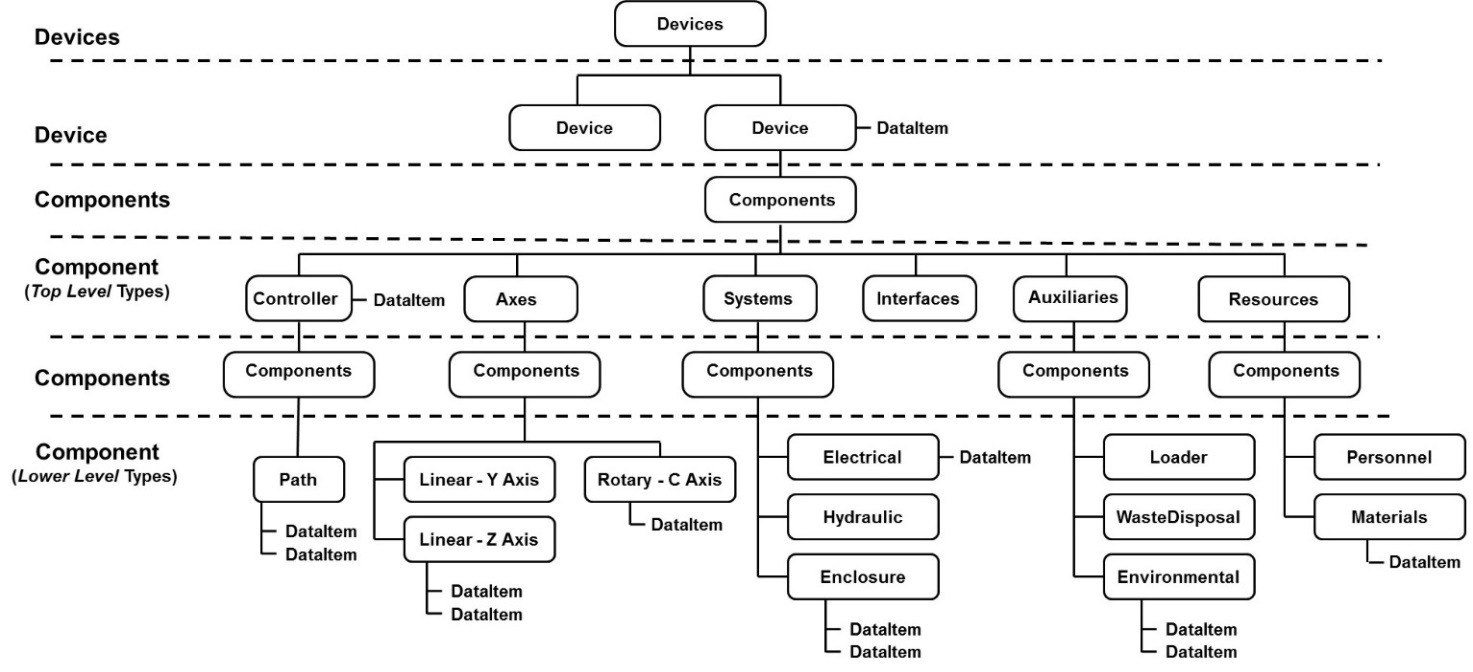
\includegraphics[width=.75\textwidth]{figures/data-entities-example-device.png}
  \caption{Example Data Entities for Device (DataItem)}
  \label{fig:data-entities-example-device}
\end{figure}

\subsection{DataItems}

The \gls{dataitems} \gls{xml} element is the first, or highest, level container for the \glspl{data entity} associated with a \gls{device} or \gls{component} \gls{xml} element.  \gls{dataitems} \must contain only \gls{dataitem} type elements.  \gls{dataitems} \must contain at least one \gls{dataitem} type element, but \may contain multiple \gls{dataitem} type elements.

\tabulinesep = 5pt
\begin{longtabu} to \textwidth {
    |l|X[3l]|X[0.75l]|}
\caption{MTConnect DataItems Element} \label{table:mtconnect-dataitems-element} \\

\hline
Element & Description & Occurrence \\
\hline
\endfirsthead

\hline
\multicolumn{3}{|c|}{Continuation of Table \ref{table:mtconnect-dataitems-element}}\\
\hline
Element & Description & Occurrence \\
\hline
\endhead
 
\gls{dataitems}
&
\glsentrydesc{dataitems}
\newline Only one \gls{dataitems} container \MUST appear for each \gls{structural element} in the XML document.
&
0..1 \\
\hline


\end{longtabu}

\subsection{DataItem}

A \gls{dataitem} \gls{xml} element represents each \gls{data entity} that \may be reported by a piece of equipment through an \gls{agent}.   \gls{dataitem} provides a detailed description for each \gls{data entity} that is reported and defines the type of data being reported along with an array of optional attributes that further define that data.  \gls{xml} elements representing \gls{dataitem} will include elements such as \gls{temperature sample}, \gls{pressure sample}, and \gls{velocity sample}. 

\tabulinesep = 5pt
\begin{longtabu} to \textwidth {
    |l|X[3l]|X[0.75l]|}
\caption{MTConnect DataItem Element} \label{table:mtconnect-dataitem-element} \\

\hline
Element & Description & Occurrence \\
\hline
\endfirsthead

\hline
\multicolumn{3}{|c|}{Continuation of Table \ref{table:mtconnect-dataitem-element}}\\
\hline
Element & Description & Occurrence \\
\hline
\endhead
 
\gls{dataitem}	
&
\glsentrydesc{dataitem}
&
1..* \\
\hline


\end{longtabu}


\subsubsection{XML Schema Structure for DataItem}

\fig{dataitem-schema-diagram} represents the structure of a \gls{dataitem} \gls{xml} element showing the attributes defined for \gls{dataitem} and the elements that may be associated with \gls{dataitem} type \gls{xml} elements.

\begin{figure}[ht]
  \centering
  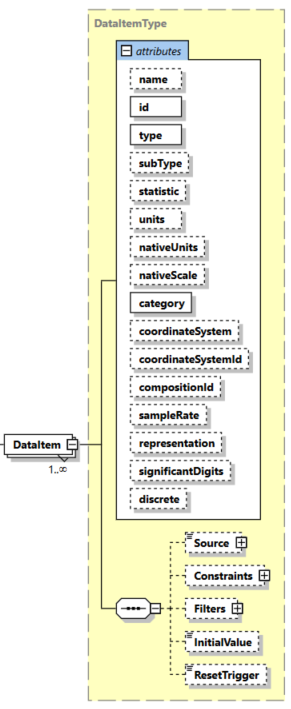
\includegraphics[width=.45\textwidth]{figures/dataitem-schema-diagram.png}
  \caption{DataItem Diagram}
  \label{fig:dataitem-schema-diagram}
\end{figure}
\FloatBarrier

\subsubsection{Attributes for DataItem}
\label{sec:Attributes for DataItem}

\tbl{attributes-for-dataitem} lists the attributes defined to provide information for a \gls{dataitem} type \gls{xml} element.  

\gls{dataitem} \must specify the type of data being reported, the id of the \gls{dataitem}, and the \gls{category} of the \gls{dataitem}.  

\tabulinesep = 5pt
\begin{longtabu} to \textwidth {
    |l|X[3l]|X[0.75l]|}
\caption{Attributes for DataItem} \label{table:attributes-for-dataitem} \\

\hline
Attribute & Description & Occurrence \\
\hline
\endfirsthead

\hline
\multicolumn{3}{|c|}{Continuation of Table \ref{table:attributes-for-dataitem}}\\
\hline
Attribute & Description & Occurrence \\
\hline
\endhead

\gls{name}
&
The name of the data item.
\newline \gls{name} is provided as an additional human readable identifier for this data item in addition to the \gls{id}.
\newline \gls{name} is an optional attribute and will be implementation dependent.
\newline An \gls{nmtoken} XML type.
&
0..1 \\
\hline

\gls{id} 
&
\glsentrydesc{id}
\newline \gls{id} is a required attribute.
\newline The \gls{id} attribute \MUST be unique within the
\gls{mtconnectdevices} document.
\newline An XML ID-type.
&
1 \\
\hline

\gls{type}
&
The type of data being measured.
\newline \gls{type} is a required attribute.
\newline Examples of types are \gls{position sample}, \gls{velocity sample}, \gls{angle sample}, \gls{block event}, and \gls{rotaryvelocity sample}.
&
1 \\
\hline

\gls{subtype}
&
A sub-categorization of the data item \gls{type}.
\newline \gls{subtype} is an optional attribute.
\newline For example, the \gls{subtype} of \gls{position sample} can be \gls{actual subtype} or \gls{commanded subtype}.
\newline Not all \gls{type} attributes have a \gls{subtype}. 
&
0..1 \\
\hline

\gls{statistic}
&
Describes the type of statistical calculation performed on a series of data samples to provide the reported data value.
\newline \gls{statistic} is an optional attribute.
\newline Examples of \gls{statistic} are \gls{average}, \gls{minimum value}, \gls{maximum value}, \gls{rootmeansquare}, \gls{range}, \gls{median}, \gls{mode}, and \gls{standarddeviation}.
&
0..1 \\
\hline

\gls{units}
&
The unit of measurement for the reported value of the data item.
\newline \gls{units} is an optional attribute.
\newline Data items in the \gls{sample} category \MUST report the standard units for the measured values.
\newline See \sect{units Attribute for DataItem} for a list of available standard units identified in the MTConnect Standard.
&
0..1 \\
\hline

\gls{nativeunits}
&
The native units of measurement for the reported value of the data item.
\newline \gls{nativeunits} is an optional attribute.
\newline See \sect{nativeUnits Attribute for DataItem} for a list of available native units identified in the MTConnect Standard.
&
0..1 \\
\hline

\gls{nativescale}
&
The \gls{nativeunits} may not be scaled to directly represent the original measured value. \gls{nativescale} \MAY be used to convert the reported value to represent the original measured value.
\newline \gls{nativescale} is an optional attribute.
\newline As an example, the \gls{nativeunits} may be reported as
\gls{gallonperminute}. The measured value may actually be in 1000  \gls{gallonperminute}. The value of the reported data \MAY be divided by the \gls{nativescale} to convert the reported value to its original measured value and units.
\newline If provided, the value \MUST be numeric.
&
0..1 \\
\hline

\gls{category}
&
\glsentrydesc{category}
\newline \gls{category} is a required attribute.
\newline The available options are \gls{sample}, \gls{event}, or \gls{condition}.
&
1 \\
\hline

\gls{coordinatesystem}
&
\glsentrydesc{coordinatesystem}
\newline \gls{coordinatesystem} is an optional attribute.
\newline The available values for \gls{coordinatesystem} are \gls{work} and \gls{machine}.
&
0..1 \\
\hline

\gls{compositionid}
&
The identifier attribute of the \gls{composition} element that the reported data is most closely associated.
\newline \gls{compositionid} is an optional attribute. 
&
0..1 \\
\hline

\gls{samplerate}
&
The rate at which successive samples of a data item are recorded by a piece of equipment.
\newline \gls{samplerate} is an optional attribute.
\newline \gls{samplerate} is expressed in terms of samples per second.
\newline If the \gls{samplerate} is smaller than one, the number can be represented as a floating point number.
\newline For example, a rate 1 per 10 seconds would be 0.1
&
0..1\\
\hline

\gls{representation}
&
Description of a means to interpret data consisting of multiple data points or as a single value.
\newline     
\newline \gls{representation} is an optional attribute.
\newline \gls{representation} defines the unique format for each set of data.
\newline \gls{representation} for \gls{timeseries representation}, \gls{discrete representation}, \gls{dataset}, and \gls{value representation} are defined in \sect{representation Attribute for DataItem}.
\newline If \gls{representation} is not specified, it \MUST be determined to be \gls{value representation}.
&
0..1 \\
\hline

\gls{significantdigits}
&
The number of significant digits in the reported value.
\newline \gls{significantdigits} is an optional attribute.
\newline This \SHOULD be specified for all numeric values.
&
0..1 \\
\hline



\gls{discrete}
&
An indication signifying whether each value reported for the \gls{data entity} is significant and whether duplicate values are to be suppressed.
\newline The value defined \MUST be either \gls{true removed} or \gls{false removed} - an XML boolean type.
\newline \gls{true removed} indicates that each update to the \gls{data entity}'s value is significant and duplicate values \MUSTNOT be suppressed.
\newline \gls{false removed} indicates that duplicated values \MUST be suppressed.
\newline If a value is not defined for \gls{discrete}, the default value \MUST be \gls{false removed}.
&
0..1 \\
\hline\end{longtabu}

\paragraph{name Attribute for DataItem}\mbox{}

The attribute \gls{name} is provided as an additional human readable identifier for a data item.  It is not required and is implementation dependent.

\paragraph{id Attribute for DataItem}\mbox{}

Each \gls{dataitem} element \must be identified with an \gls{id}.   The \gls{id} attribute \must be unique across the entire \gls{mtconnectdevices} document for a piece of equipment, including the identifiers for all \glspl{structural element}.  This unique \gls{id} provides the information required by a client software application to uniquely identify each \gls{data entity}.

For example, an \gls{xml} document may provide three different \glspl{data entity} representing the position of the axes on a machine (x axis position, y axis position, and z axis position).  All three may be modeled in the \gls{xml} document as \gls{position sample} type data items for the \gls{axes} components.  The unique \gls{id} allows the client software application to distinguish the data for each of the axes.

\newpage

\paragraph{type and subType Attributes for DataItem}\mbox{}

The attribute \gls{type} specifies the kind of data that is represented by the data item.

The attribute \gls{type} \must be specified for every data item.

A data item \may further qualify the data being reported by specifying a \gls{subtype}.  \gls{subtype} is required for certain data item \glspl{type}.  For example, \gls{position sample} has the \gls{subtype} of \gls{actual subtype} and \gls{programmed subtype}.  Both data values can be represented in the document as two separate and different \gls{dataitem} \gls{xml} elements – \gls{position sample} with \gls{subtype} \gls{actual subtype} and \gls{position sample} with \gls{subtype} \gls{programmed subtype}.

The \gls{type} and \gls{subtype} \should be used to further identify the meaning of the \gls{dataitem} associated with a \gls{component} element when a \gls{subtype} is applicable.  There \shouldnot be more than one \gls{dataitem} with the same \gls{type}, \gls{subtype}, and \gls{compositionid} within a \gls{component} element.

\sect{Listing of Data Items} provides a detailed listing of the data item \gls{type} and \gls{subtype} elements defined for each \gls{category} of data item available for a piece of equipment: \gls{sample category}, \gls{event category}, and \gls{condition category}.

\paragraph{statistic Attribute for DataItem}\mbox{}

A piece of equipment may further process some data types using a statistical calculation like average, mean, or square root.  In this case, the \gls{statistic} attribute \may be used to indicate how the data was processed.  

\gls{statistic} may be defined for any \gls{sample category} type \gls{dataitem}.   All statistic data is reported in the standard units of the \gls{dataitem}.

\gls{statistic} data is always the result of a calculation using data that has been measured over a specified period of time. 

The value of \gls{statistic} may be periodically reset.   When a piece of equipment reports a \gls{dataitem} with a value that is a \gls{statistic}, the information provided in the \gls{xml} document for that \gls{data entity} \must include an additional attribute called \gls{duration}.   The attribute \gls{duration} defines the period of time over which the \gls{statistic} has been calculated.   See \citetitle{MTCPart3} for more information about \gls{duration}.

\tbl{dataitem-attribute-statistic-type} shows the \gls{statistic} calculations that can be defined for a \gls{dataitem}.

\tabulinesep = 5pt
\begin{longtabu} to \textwidth {
    |l|X[3l]|}
\caption{DataItem attribute statistic type} \label{table:dataitem-attribute-statistic-type} \\

\hline
Statistic & Description\\
\hline
\endfirsthead

\hline
\multicolumn{2}{|c|}{Continuation of Table \ref{table:dataitem-attribute-statistic-type}}\\
\hline
Statistic & Description\\
\hline
\endhead
 
\gls{average} & \glsentrydesc{average} \\ \hline

\gls{kurtosis} & \glsentrydesc{kurtosis} \\ \hline

\gls{maximum value} &
Maximum or peak value recorded for the data item during the calculation period.\\ \hline

\gls{median} & \glsentrydesc{median} \\ \hline

\gls{minimum value} &
Minimum value recorded for the data item during the calculation period.\\ \hline

\gls{mode} & \glsentrydesc{mode} \\ \hline

\gls{range} & \glsentrydesc{range} \\ \hline

\gls{rootmeansquare} & \glsentrydesc{rootmeansquare} \\ \hline

\gls{standarddeviation} & \glsentrydesc{standarddeviation} \\ \hline

\end{longtabu}


\pagebreak

\paragraph{units Attribute for DataItem}\label{sec:units Attribute for DataItem}\mbox{}

\tbl{dataitem-attribute-units-type} lists the units that are defined as the standard unit of measure for each type of \gls{dataitem}.  All \gls{sample category} type data items \must report data values in standard units.     

\tabulinesep = 5pt
\begin{longtabu} to \textwidth {
    |l|X[3l]|}
\caption{DataItem attribute units type} \label{table:dataitem-attribute-units-type} \\

\hline
Units & Description\\
\hline
\endfirsthead

\hline
\multicolumn{2}{|c|}{Continuation of Table \ref{table:dataitem-attribute-units-type}}\\
\hline
Units & Description\\
\hline
\endhead
 
\gls{ampere} & \glsentrydesc{ampere} \\ \hline

\gls{celsius} & \glsentrydesc{celsius} \\ \hline

\gls{count} & \glsentrydesc{count} \\ \hline


\gls{cubicmillimeter}
&
Geometric volume in millimeters \\
\hline

\gls{cubicmillimeterpersecond}
&
Change of geometric volume per second \\
\hline

\gls{cubicmillimeterpersecondsquared}
&
Change in geometric volume per second squared \\
\hline

\gls{decibel} & \glsentrydesc{decibel} \\ \hline

\gls{degree} & \glsentrydesc{degree} \\ \hline

\gls{degreepersecond} & \glsentrydesc{degreepersecond} \\ \hline

\gls{degreepersecondsquared} & \glsentrydesc{degreepersecondsquared} \\ \hline

\gls{hertz} & \glsentrydesc{hertz} \\ \hline

\gls{joule} & \glsentrydesc{joule} \\ \hline

\gls{kilogram} & \glsentrydesc{kilogram} \\ \hline

\gls{liter} &  \glsentrydesc{liter} \\ \hline

\gls{literpersecond} & \glsentrydesc{literpersecond} \\ \hline

\gls{microradian} & \glsentrydesc{microradian} \\ \hline

\gls{milligram}
&
Milligram  \\
\hline

\gls{milligrampercubicmillimeter}
&
Milligram per cubic millimeter   \\
\hline

\gls{milliliter}
&
Milliliter   \\
\hline


\gls{millimeter} & \glsentrydesc{millimeter} \\ \hline

\gls{millimeterperrevolution}
&
\glsentrydesc{millimeterperrevolution}
 \\
\hline

\gls{millimeterpersecond} & \glsentrydesc{millimeterpersecond} \\ \hline

\gls{millimeterpersecondsquared} & \glsentrydesc{millimeterpersecondsquared} \\ \hline

\gls{millimeter3d} & \glsentrydesc{millimeter3d} \\ \hline

\gls{newton} & \glsentrydesc{newton} \\ \hline

\gls{newtonmeter} & \glsentrydesc{newtonmeter} \\ \hline

\gls{ohm} & \glsentrydesc{ohm} \\ \hline

\gls{pascal} & \glsentrydesc{pascal} \\ \hline

\gls{pascalsecond} & \glsentrydesc{pascalsecond} \\ \hline

\gls{percent} & \glsentrydesc{percent} \\ \hline

\gls{ph sample}
&
A measure of the acidity or alkalinity of a solution. \\ \hline

\gls{revolutionperminute} & \glsentrydesc{revolutionperminute} \\ \hline

\gls{second} & \glsentrydesc{second} \\ \hline

\gls{siemenspermeter} & \glsentrydesc{siemenspermeter} \\ \hline

\gls{volt} & \glsentrydesc{volt} \\ \hline

\gls{voltampere sample} & Volt-Ampere (VA) \\ \hline

\gls{voltamperereactive sample} & Volt-Ampere Reactive (VAR) \\ \hline

\gls{watt} & \glsentrydesc{watt} \\ \hline

\gls{wattsecond} & \glsentrydesc{wattsecond} \\ \hline


\end{longtabu}

\paragraph{nativeUnits Attribute for DataItem}\label{sec:nativeUnits Attribute for DataItem}\mbox{}

The \gls{nativeunits} attribute provides additional information about the original measured value for a \gls{data entity} reported by a piece of equipment.  \gls{nativeunits} \may be specified to provide additional information about the data if the units of the measured value supplied by the piece of equipment differ from the value provided for that data when converted to standard units.

\tbl{dataitem-attribute-nativeunits-type} defines the \gls{nativeunits} currently supported by the \gls{mtconnectdevices} \gls{xml} document:

\tabulinesep = 5pt
\begin{longtabu} to \textwidth {
    |l|X[3l]|}
\caption{DataItem attribute nativeunits type} \label{table:dataitem-attribute-nativeunits-type} \\

\hline
Native Units & Description\\
\hline
\endfirsthead

\hline
\multicolumn{2}{|c|}{Continuation of Table \ref{table:dataitem-attribute-nativeunits-type}}\\
\hline
Native Units & Description\\
\hline
\endhead
 
\gls{centipoise} & \glsentrydesc{centipoise} \\ \hline

\gls{degreeperminute} & \glsentrydesc{degreeperminute} \\ \hline

\gls{fahrenheit} & \glsentrydesc{fahrenheit} \\ \hline

\gls{foot} & \glsentrydesc{foot} \\ \hline

\gls{footperminute} & \glsentrydesc{footperminute} \\ \hline

\gls{footpersecond} & \glsentrydesc{footpersecond} \\ \hline

\gls{footpersecondsquared} & \glsentrydesc{footpersecondsquared} \\ \hline

\gls{foot3d} & \glsentrydesc{foot3d} \\ \hline

\gls{gallonperminute} & \glsentrydesc{gallonperminute} \\ \hline

\gls{hour}
&
A measurement of time in hours \\
\hline

\gls{inch} & \glsentrydesc{inch} \\ \hline

\gls{inchperminute} & \glsentrydesc{inchperminute} \\ \hline

\gls{inchpersecond} & \glsentrydesc{inchpersecond} \\ \hline

\gls{inchpersecondsquared} & \glsentrydesc{inchpersecondsquared} \\ \hline

\gls{inch3d} & \glsentrydesc{inch3d} \\ \hline

\gls{inchpound} & \glsentrydesc{inchpound} \\ \hline

\gls{kelvin} & \glsentrydesc{kelvin} \\ \hline

\gls{kilowatt} & \glsentrydesc{kilowatt} \\ \hline

\gls{kilowatthour} & \glsentrydesc{kilowatthour} \\ \hline

\gls{liter} & \glsentrydesc{liter} \\ \hline

\gls{literperminute} & \glsentrydesc{literperminute} \\ \hline

\gls{millimeterperminute} & \glsentrydesc{millimeterperminute} \\ \hline

\gls{minute}
&
A measurement of time in minutes \\
\hline

\gls{other} & \glsentrydesc{other} \\ \hline

\gls{pound} & \glsentrydesc{pound} \\ \hline

\gls{poundperinchsquared} & \glsentrydesc{poundperinchsquared} \\ \hline

\gls{radian} & \glsentrydesc{radian} \\ \hline

\gls{radianperminute} & \glsentrydesc{radianperminute} \\ \hline

\gls{radianpersecond} & \glsentrydesc{radianpersecondsquared} \\ \hline

\gls{radianpersecondsquared} & \glsentrydesc{radianpersecondsquared} \\ \hline

\gls{revolutionpersecond} & \glsentrydesc{revolutionpersecond} \\ \hline

\end{longtabu}

\paragraph{nativeScale Attribute for DataItem}\mbox{}

The units of measure for some measured values may be different from the \gls{nativeunits} defined in \sect{category Attribute for DataItem}.   In the cases where the units of measure use a different weighting or range than is provided by \gls{nativeunits}, the \gls{nativescale} attribute can be used to define the original units of measure.

As an example, a velocity measured in units of 100 ft/min can be represented as \cfont{nativeUnits="FEET/MINUTE"} and \cfont{nativeScale="100"}. 

\paragraph{category Attribute for DataItem}
\label{sec:category Attribute for DataItem}\mbox{}

Many \gls{dataitem} types provide two forms of data, a value (reported as either a \gls{sample category} or \gls{event category} category) and a health status (reported as a \gls{condition category} category).  Therefore, each occurrence of a \gls{dataitem} in the \gls{xml} document \must report a \gls{category} attribute.  This \gls{category} attribute provides the information required by a client software application to determine the specific meaning of the data provided.

\newpage

Each \gls{data entity} provided by a piece of equipment \must be identified with one of the following: \gls{sample category}, \gls{event category}, \gls{condition category}.

A \gls{sample category} is the reading of the value of a continuously variable or analog data value.  A continuous value can be measured at any point-in-time and will always produce a result.  An example of a continuous data value is the position of a linear axis called X.   

The data provided for a \gls{sample category} category data item is always a floating point number or integers that have an infinite number of possible values.  This is different from a state or discrete type data item that has a limited number of possible values.  A data item of category \gls{sample category} \must also provide the \gls{units} attribute.



An \gls{event category} is a data item representing a discrete piece of information from the piece of equipment.  \gls{event category} does not have intermediate values that vary over time, as does \gls{sample category}.   An \gls{event category} is information that, when provided at any specific point in time, represents the current state of the piece of equipment.

There are two types of \gls{event category}: those representing state, with two or more discrete values, and those representing messages that contain plain text data.

An example of a state type \gls{event category} is the value of the data item \gls{doorstate event}, which can be \gls{open value}, \gls{closed value}, or \gls{unlatched value}.   (Note:  No other values are valid to represent the value of \gls{doorstate event}.)

An example of a message type \gls{event category} is the value for a data item \gls{program event}.  The value representing \gls{program event} can be any valid string of characters.



A \gls{condition category} is a data item that communicates information about the health of a piece of equipment and its ability to function.  A valid value for a data item in the category \gls{condition category} can be one of \gls{normal}, \gls{warning}, or \gls{fault}.

A data item of category \gls{condition category} \may report multiple values (\gls{condition category}) at one time whereas a data item of category \gls{sample category} or \gls{event category} can only have a single value at any one point in time.

\newpage

\paragraph{coordinateSystem Attribute for DataItem}\mbox{}

The values reported by a piece of equipment for some types of data will be associated to a specific positioning measurement system used by the equipment.  The \gls{coordinatesystem} attribute \may be used to specify the coordinate system used for the measured value.

The \gls{coordinatesystem} attribute is used by a client software application to interpret the spatial relationship between values reported by a piece of equipment.

If \gls{coordinatesystem} is not provided, all values representing positional data for \gls{axes} \must be interpreted using the \gls{machine} coordinate system and all values representing positional data for \gls{path} \must be interpreted using the \gls{work} coordinate system.

\tbl{dataitem-attribute-coordinatesystem} defines the types of \gls{coordinatesystem} currently supported by the \gls{mtconnectdevices} \gls{xml} document:

\tabulinesep = 5pt
\begin{longtabu} to \textwidth {
    |l|X[3l]|}
\caption{DataItem attribute coordinateSystem type} \label{table:dataitem-attribute-coordinatesystem} \\

\hline
Coordinate System & Description\\
\hline
\endfirsthead

\hline
\multicolumn{2}{|c|}{Continuation of Table \ref{table:dataitem-attribute-coordinatesystem}}\\
\hline
Coordinate System & Description\\
\hline
\endhead
 
\gls{machine}
&
\glsentrydesc{machine} \\ 
\hline

\gls{work}
&
\glsentrydesc{work} \\
\hline


\end{longtabu}



\paragraph{compositionId Attribute for DataItem}\mbox{}

\gls{compositionid} attribute identifies the id of the \gls{composition} element where the reported data is most closely associated.

An example would be a \gls{temperature sample} associated with a \gls{linear} type axis may be further clarified by referencing the \gls{motor} or \gls{amplifier} type \gls{composition} element associated with that axis, which differentiates the temperature of the motor from the temperature of the amplifier.

\newpage

The \gls{compositionid} attribute provides the information required by a client software application to interpret the data with a greater specificity and to disambiguate between multiple \glspl{data entity} of the same data type associated with a \gls{component} element.

\paragraph{sampleRate Attribute for DataItem}\mbox{}

The value for some data types provided by a piece of equipment may be reported as a single set of data containing a series of values that have been recorded at a fixed sample rate.  When such data is reported, the \gls{samplerate} defines the rate at which successive samples of data were recorded.

The \gls{samplerate} attribute provides the information required by a client software application to interpret the data and the sampling time relationship between successive values contained in the set of data.

\gls{samplerate} is expressed in terms of samples per second.  If the sample rate is smaller than one, the number can be represented as a floating point number.  For example, a rate 1 per 10 seconds would be 0.1

\paragraph{representation Attribute for DataItem}\label{sec:representation Attribute for DataItem}\mbox{}

Some data types provide data that may consist of a series of values or a file of data, not a single value.  Other data types provide a series of data values that may require additional information so that the data may be correctly understood by a client software application.

When such data is provided, the \gls{representation} attribute \must be used to define the format for the data provided.

The types of \gls{representation} defined are provided in \tbl{dataitem-attribute-representation-type}.

\begin{note}
Note:  See \citetitle{MTCPart3} for more information on the structure and format of each \gls{representation}.

\end{note}

\tabulinesep = 5pt
\begin{longtabu} to \textwidth {
    |l|X[3l]|}
\caption{DataItem attribute representation type} \label{table:dataitem-attribute-representation-type} \\

\hline
Representation & Description\\
\hline
\endfirsthead

\hline
\multicolumn{2}{|c|}{Continuation of Table \ref{table:dataitem-attribute-representation-type}}\\
\hline
Representation & Description\\
\hline
\endhead
 


\gls{dataset}
&
The reported value(s) are represented as a set of \textit{key-value pairs}.
\newline Each reported value in the \gls{data set} \MUST have a unique key.  \\
\hline

\gls{discrete representation}
&
\DEPRECATED as a \gls{representation} in MTConnect Version. 1.5.  Replaced by the \gls{discrete} attribute for a \gls{data entity} – \sect{discrete-attribute}. \newline \deprecated{A Data Entity where each discrete occurrence of the data may have the same value as the previous occurrence of the data.  There is no reported state change between occurrences of the data.   
\newline In this case, duplicate occurrences of the same data value SHOULD NOT be suppressed. 
\newline An example of a DISCRETE data type would be a parts counter that reports the completion of each part versus the accumulation of parts.   
Another example would be a Message that does not typically have a reset state and may re-occur each time a specific message is triggered.} 
 \\
\hline


\gls{timeseries representation}
&
\glsentrydesc{timeseries representation}
\newline The data is reported for a specified number of samples and each sample is reported with a fixed period.
\\
\hline


\gls{value representation}
&
\glsentrydesc{value representation}
\newline If no representation is specified for a data item, the representation \MUST be determined to be \gls{value representation}.\\
\hline

\end{longtabu}

\pagebreak

\paragraph{significantDigits Attribute for DataItem}\mbox{}

\gls{significantdigits} is used to specify the level of precision (number of significant digits) for the value provided for a data item.

\gls{significantdigits} attribute is not required for a data item, but it is recommended and \should be used for any data item reporting a numeric value.

\paragraph{discrete Attribute for DataItem}\label{sec:discrete-attribute}\mbox{}

An indication signifying whether each value reported for the \gls{data entity} is significant and whether duplicate values are to be suppressed.

The value defined \MUST be either \gls{true removed} or \gls{false removed} - an XML boolean type.

\gls{true removed} indicates that each update to the \gls{data entity}'s value is significant and duplicate values \MUSTNOT be suppressed.

\gls{false removed} indicates that duplicated values \MUST be suppressed.

If a value is not defined for \gls{discrete}, the default value \MUST be \gls{false removed}.

\subsubsection{Elements for DataItem}

\tbl{elements-for-dataitem} lists the elements defined to provide additional information for a \gls{dataitem} type \gls{xml} element.

\tabulinesep = 5pt
\begin{longtabu} to \textwidth {
    |l|X[3l]|X[0.75l]|}
\caption{Elements for DataItem} \label{table:elements-for-dataitem} \\

\hline
Element & Description & Occurrence \\
\hline
\endfirsthead

\hline
\multicolumn{3}{|c|}{Continuation of Table \ref{table:elements-for-dataitem}}\\
\hline
Element & Description & Occurrence \\
\hline
\endhead

\gls{source}
&
\gls{source} is an optional XML element that identifies the \gls{component}, \gls{dataitem}, or \gls{composition} representing the area of the piece of equipment from which a measured value originates.
\newline Additionally, \gls{source} \MAY provide information relating to the identity of a measured value.  This information is reported as CDATA for \gls{source}. (example, a PLC tag)
&
0..1 \\
\hline

\gls{constraints}
&
\glsentrydesc{constraints}
 \gls{constraints} are used by a software application to evaluate the validity of the reported data.
&
0..1 \\
\hline

\gls{filters}
&
An optional container for the \gls{filter} elements associated with this \gls{dataitem} element. 
&
0..1 \\
\hline

\gls{initialvalue}
&
\glsentrydesc{initialvalue}
\newline Only one \gls{initialvalue} element may be defined for a data item. The value will be constant and cannot change.
\newline If no \gls{initialvalue} element is defined for a data item that is periodically reset, then the starting value for the data item \MUST be a value of 0.
&
0..1 \\
\hline

\gls{resettrigger}
&
\glsentrydesc{resettrigger}
&
0..1 \\
\hline

\end{longtabu}

\paragraph{Source Element for DataItem}\mbox{}

\gls{source} is an optional \gls{xml} element that may be used to identify the physical part of a piece of equipment where the data represented by \gls{dataitem} originated and/or it may be used to identify a complex name or an alternate name used to identify the data where it originated (e.g. a PLC tag name).


As an example, data related to a servo motor on an \gls{axes} component may actually originate from a measurement made in the \gls{controller} element.

In the case where the real name associated with a \gls{dataitem} element is either complex or does not meet the format requirements of a NMTOKEN \gls{xml} type, the real name of the element may not be able to be expressed in the \gls{name} attribute. Additionally, a second or alternate name may be required to describe a piece of data. An example of this case would be the identity of the bit address in a PLC that represents this piece of data (PLC address I0015.4). When these cases occur, the alternate name can be provided as the value for the \gls{cdata} for \gls{source}.

The \gls{xml} schema in \fig{source-schema-diagram} represents the structure of the \gls{source} \gls{xml} element showing the attributes defined for \gls{source}.

\begin{figure}[ht]
  \centering
  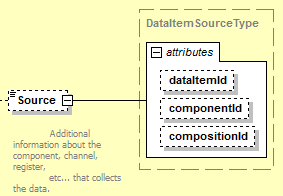
\includegraphics[width=.5\textwidth]{figures/source-schema-diagram.png}
  \caption{Source Diagram}
  \label{fig:source-schema-diagram}
\end{figure}
\FloatBarrier

\subparagraph{Attributes for Source} \mbox{}

\tbl{attributes-for-source} identifies the attributes available to identify \gls{source} for a measured value:

\tabulinesep = 5pt
\begin{longtabu} to \textwidth {
    |l|X[3l]|X[0.75l]|}
\caption{Attributes for Source} \label{table:attributes-for-source} \\

\hline
Attribute & Description & Occurrence \\
\hline
\endfirsthead

\hline
\multicolumn{3}{|c|}{Continuation of Table \ref{table:attributes-for-source}}\\
\hline
Attribute & Description & Occurrence \\
\hline
\endhead
 
\gls{componentid} 
&
\glsentrydesc{componentid}
\newline A \gls{valid data value} reported for \gls{componentid} \MUST be the value of the \gls{id} attribute for the \gls{component} element identified.\newline \gls{componentid} is an optional attribute.
&
0..1\\
\hline

\gls{dataitemid} 
&
\glsentrydesc{dataitemid}
\newline A \gls{valid data value} reported for \gls{dataitemid} \MUST be the value of the \gls{id} attribute for the \gls{dataitem} element identified.
\newline \gls{dataitemid} is an optional attribute.
&
0..1\\
\hline

\gls{compositionid} 
&
The identifier attribute of the \gls{composition} element that represents the physical part of a piece of equipment where the data represented by the \gls{dataitem} element originated.
\newline A \gls{valid data value} reported for \gls{compositionid} \MUST be the value of the \gls{id} attribute for the \gls{composition} element identified.
\newline \gls{compositionid} is an optional attribute.
&
0..1\\
\hline

\end{longtabu}

\begin{note}
Note: \notesign One of componentID, componsitionId , or dataItemId MUST be provided.

\end{note}


\paragraph{Constraints Element for DataItem}\mbox{}

For some types of \gls{dataitem} elements, the expected value(s) for the data reported for the \gls{dataitem} \may be restricted to specific values or a range of values.

\gls{constraints} is an optional \gls{xml} element that provides a way to define the expected value(s) or the upper and lower limits for the range of values that are expected to be reported in response to a \gls{current request} or \gls{sample request}.

\gls{constraints} are used by a software application to evaluate the validity of the data reported.

The value associated with each \gls{constraint} element is reported in the \gls{cdata} for that element.

\subparagraph{Schema for Constraints} \mbox{}

The \gls{xml} schema in \fig{constraints-schema-diagram} represents the structure of the \gls{constraints} \gls{xml} element and the elements defined for \gls{constraints}.

\begin{figure}[ht]
  \centering
  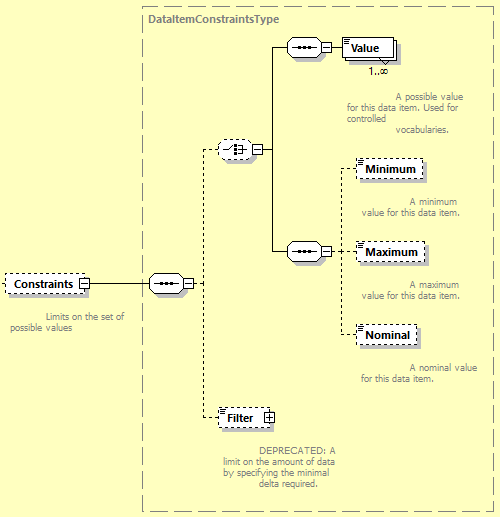
\includegraphics[width=.75\textwidth]{figures/constraints-schema-diagram.png}
  \caption{Constraints Diagram}
  \label{fig:constraints-schema-diagram}
\end{figure}
\FloatBarrier

\tbl{elements-for-constraints} identifies the elements available to identify \gls{constraints} for a measured value:

\tabulinesep = 5pt
\begin{longtabu} to \textwidth {
    |l|X[3l]|X[0.75l]|}
\caption{Elements for Constraints} \label{table:elements-for-constraints} \\

\hline
Element & Description & Occurrence \\
\hline
\endfirsthead

\hline
\multicolumn{3}{|c|}{Continuation of Table \ref{table:elements-for-constraints}}\\
\hline
Element & Description & Occurrence \\
\hline
\endhead

\gls{value}
&
\gls{value} represents a single data value that is expected to be reported for a \gls{dataitem} element.
\newline The data value is provided in the \gls{cdata} for this element and may be any numeric or text content.
\newline When there are multiple data values that may be expected to be reported for a \gls{dataitem} element, multiple \gls{value} elements may be defined.
\newline In the case where only one \gls{value} element is defined, the data returned in response to a \gls{current request} or \gls{sample request} request \MUST be the data value defined for \gls{value} element.
\newline \gls{value} \MUSTNOT be used in conjunction with any other \gls{constraint} elements.
&
0..* \\
\hline

\gls{maximum}
&
If the data reported for a data item is a range of numeric values, the expected value reported \MAY be described with an upper limit defined by this constraint.
\newline The data value is provided in the \gls{cdata} for this element and \MUST be a value using the same units as the reported data. 
&
0..1 \\
\hline

\gls{minimum}
&
If the data reported for a data item is a range of numeric values, the expected value reported \MAY be described with a lower limit defined by this constraint.
\newline The data value is provided in the \gls{cdata} for this element and \MUST be a value using the same units as the reported data. 
&
0..1 \\
\hline

\gls{nominal}
&
The target or expected value for this data item.
\newline The data value is provided in the \gls{cdata} for this element and \MUST be a value using the same units as the reported data. 
&
0..1 \\
\hline


\deprecated{\gls{filter}}
&
\DEPRECATED in Version 1.4 – Moved to the \gls{filters} element of a \gls{dataitem}.
\newline \deprecated{If the data reported for a DataItem is a numeric value, a new value MUST NOT be reported if the change from the last reported value is less than the delta given as the CDATA of this element. Filter is an abstract type XML element. As such, Filter will never appear in the XML document, but will be replaced by a Filter type. The only currently supported Filter type is MINIMUM_DELTA. The CDATA MUST be an absolute value using the same Units as the reported data. Additional filter types MAY be supported in the future.}
&
0..1 \notesign
\\ \hline

\end{longtabu}

\begin{note}
Note: \notesign Remains in schema for backwards compatibility.

\end{note}

\paragraph{Filters Element for DataItem}\mbox{}

\gls{filters} is an optional \gls{xml} container that organizes the \gls{filter} elements for \gls{dataitem}.

\gls{filters} contains one or more \gls{filter} \gls{xml} elements.

\tabulinesep = 5pt
\begin{longtabu} to \textwidth {
    |l|X[3l]|X[0.75l]|}
\caption{MTConnect Filters Element} \label{table:mtconnect-filters-element} \\

\hline
Element & Description & Occurrence \\
\hline
\endfirsthead

\hline
\multicolumn{3}{|c|}{Continuation of Table \ref{table:mtconnect-filters-element}}\\
\hline
Element & Description & Occurrence \\
\hline
\endhead
 
\gls{filters}	
&
\glsentrydesc{filters}
 Only one \gls{filters} container \MAY appear for a \gls{dataitem} element.
&
0..1 \\
\hline


\end{longtabu}

\newpage

\subparagraph{Filter} \mbox{}

\gls{filter} provides a means to control when an \gls{agent} records updated information for a data item.  Currently, there are two types of \gls{filter} elements defined in the MTConnect Standard - \gls{minimumdelta} and \gls{period}.   More \gls{filter} types may be added in the future.

The value associated with each \gls{filter} element is reported in the \gls{cdata} for that element.

\fig{filter-schema-diagram} represents the structure for \gls{filter} \gls{xml} element.

\begin{figure}[ht]
  \centering
  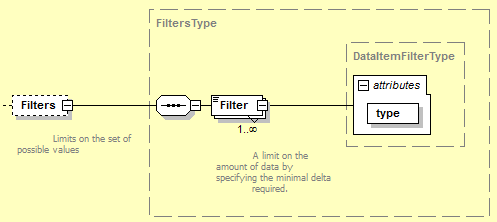
\includegraphics[width=.75\textwidth]{figures/filter-schema-diagram.png}
  \caption{Filter Diagram}
  \label{fig:filter-schema-diagram}
\end{figure}
\FloatBarrier

\tbl{dataitem-element-filter-type} describes the types of \gls{filter} defined for a \gls{dataitem} element and the expected behavior of an \gls{agent} when a \gls{filter} is applied to \gls{dataitem} element.

\tabulinesep = 5pt
\begin{longtabu} to \textwidth {
    |l|X[3l]|X[0.75l]|}
\caption{DataItem Element Filter type} \label{table:dataitem-element-filter-type} \\

\hline
type & Description & Occurrence \\
\hline
\endfirsthead

\hline
\multicolumn{3}{|c|}{Continuation of Table \ref{table:dataitem-element-filter-type}}\\
\hline
type & Description & Occurrence \\
\hline
\endhead
 
\gls{minimumdelta}
&
For a \gls{minimumdelta} type \gls{filter}, a new value \MUSTNOT be reported for a data item unless the measured value has changed from the last reported value by at least the delta given as the \gls{cdata} of this element.
\newline The \gls{cdata} \MUST be an absolute value using the same units as the reported data. 
&
0..1 \notesign \\
\hline

\gls{period}
&
For a \gls{period} type \gls{filter}, the data reported for a data item is provided on a periodic basis. The \gls{period} for reporting data is defined in the \gls{cdata} for the \gls{filter}.
\newline The \gls{cdata} \MUST be an absolute value reported in seconds representing the time between reported samples of the value of the data item.
\newline If the \gls{period} is smaller than one second, the number can be represented as a floating point number. For example, a \gls{period} of 100 milliseconds would be 0.1.
&
0..1 \notesign \\
\hline

\end{longtabu}

\begin{note}
\notesign Note: Either \gls{minimumdelta} or \gls{period} can be defined, not both.

\end{note}

\paragraph{InitialValue Element for DataItem}\mbox{}

\gls{initialvalue} is an \gls{xml} element that defines the value to be set for the data item after a reset event.

The value associated with the \gls{initialvalue} element is reported in the \gls{cdata} for this element and \must be an absolute value using the same units as the reported data.

\paragraph{ResetTrigger Element for DataItem}\mbox{}

The value of some data types is periodically reset to the value of the \gls{initialvalue} element.   These reset events may be based upon a specific elapsed time or may be triggered by a physical or logical reset action that causes the reset to occur.   \gls{resettrigger} provides additional information regarding the meaning of the data – establishing an understanding of the time frame that the data represents so that the data may be correctly understood by a client software application.

\tabulinesep = 5pt
\begin{longtabu} to \textwidth {
    |l|X[3l]|X[0.75l]|}
\caption{MTConnect ResetTrigger Element} \label{table:mtconnect-resettrigger-element} \\

\hline
Element & Description & Occurrence \\
\hline
\endfirsthead

\hline
\multicolumn{3}{|c|}{Continuation of Table \ref{table:mtconnect-resettrigger-element}}\\
\hline
Element & Description & Occurrence \\
\hline
\endhead
 
\gls{resettrigger}
&
\gls{resettrigger} is an XML element that describes the reset action that causes a reset to occur.
\newline It is additional information regarding the meaning of the data that establishes an understanding of the time frame that the data represents so that the data may be correctly understood by a client software application.
&
0..1 \\
\hline


\end{longtabu}


The reset action that \may cause a reset to occur is provided in the \gls{cdata} for this element. 

The reset actions that may cause a reset to occur are described in \tbl{dataitem-element-resettrigger-type}.

\tabulinesep = 5pt
\begin{longtabu} to \textwidth {
    |l|X[3l]|}
\caption{DataItem Element ResetTrigger type} \label{table:dataitem-element-resettrigger-type} \\

\hline
Reset Actions & Description\\
\hline
\endfirsthead

\hline
\multicolumn{2}{|c|}{Continuation of Table \ref{table:dataitem-element-resettrigger-type}} \\
\hline
Reset Actions & Description\\
\hline
\endhead
 
\gls{actioncomplete} & 
The value of the \gls{data entity} that is measuring an action or
operation is to be reset upon completion of that action or
operation. \\ \hline 

\gls{annual} & 
The value of the \gls{data entity} is to be reset at the end of a 12-month period.\\ \hline 

\gls{day} & 
The value of the \gls{data entity} is to be reset at the end of a 24-hour
period.\\ \hline 

\gls{life} & 
The value of the \gls{data entity} is not reset and accumulates for the
entire life of the piece of equipment.\\ \hline 

\gls{maintenance}
& 
The value of the \gls{data entity} is to be reset upon completion of a maintenance event.
\\ \hline 

\gls{month} & 
The value of the \gls{data entity} is to be reset at the end of a monthly
period. \\ \hline 

\gls{poweron} & 
The value of the \gls{data entity} is to be reset when power was
applied to the piece of equipment after a planned or unplanned
interruption of power has occurred.\\ \hline 

\gls{shift} & 
The value of the \gls{data entity} is to be reset at the end of a work
shift.\\ \hline 

\gls{week} & 
The value of the \gls{data entity} is to be reset at the end of a 7-day
period.\\ \hline 



\end{longtabu}


\section{Listing of Data Items}
\label{sec:Listing of Data Items}

In the MTConnect Standard, \gls{dataitem} elements are defined and organized based upon the \gls{category} and \gls{type} attributes.  
The \gls{category} attribute provides a high level grouping for \gls{dataitem} elements based on the kind of information that is reported by the data item.

These categories are:

\begin{itemize}

\item \gls{sample category}

A \gls{sample category} reports a continuously variable or analog data value. 

\item \gls{event category}

An \gls{event category} reports information representing a functional state, with two or more discrete values, associated with a component or it contains a message.  The data provided may be a numeric value or text.

\item \gls{condition category}

A \gls{condition category} reports information about the health of a piece of equipment and its ability to function.
\end{itemize}

The \gls{type} attribute specifies the specific kind of data that is reported.   For some types of data items, a \gls{subtype} attribute may also be used to differentiate between multiple data items of the same \gls{type} where the information reported by the data item has a different, but related, meaning.

Many types of data items provide two forms of data: a value (reported as either a \gls{sample category} or \gls{event category}) and a health status (reported as a \gls{condition category}).  These \gls{dataitem} types \may be defined in more than one \gls{category} based on the data that they report.

\newpage

\subsection{Data Items in category SAMPLE}

The types of \gls{dataitem} elements in the \gls{sample category} category report data representing a continuously changing or analog data value.  This data can be measured at any point-in-time and will always produce a result.  The data provided may be a scalar floating point number or integers that have an infinite number of possible values.  The \gls{units} attribute \must be defined and reported for each \gls{dataitem} in this category.

\tbl{dataitem-type-category-sample} defines the types and subtypes of \gls{dataitem} elements defined for the \gls{sample category} category.  The subtypes are indented below their associated types. 

\tabulinesep = 5pt
\begin{longtabu} to \textwidth {
    |X[3l]|X[3l]|X[2.8l]|}
\caption{DataItem type subType for category SAMPLE} \label{table:dataitem-type-category-sample} \\

\hline
DataItem type/subType & Description & Units\\
\hline
\endfirsthead

\hline
\multicolumn{3}{|c|}{Continuation of Table \ref{table:dataitem-type-category-sample}:  \nameref{table:dataitem-type-category-sample}}\\
\hline
DataItem type/subType & Description & Units\\
\hline
\endhead

\gls{acceleration sample}
&
Rate of change of velocity.
&
\glsentryunits{acceleration sample} \\ \hline 

\gls{accumulatedtime sample} 
& 
\glsentrydesc{accumulatedtime sample} 
\newline \DEPRECATIONWARNING:  May be deprecated in the future.  Recommend using \gls{processtimer sample} and \gls{equipmenttimer sample}.
& 
\glsentryunits{accumulatedtime sample} \\ \hline 

\gls{amperage sample} & \glsentrydesc{amperage sample} & \glsentryunits{amperage sample} \\ \hline 

\quad \gls{actual subtype}
&
The measured amperage being delivered from a power source.
&
\glsentryunits{amperage sample} \\ \hline 

\quad \gls{alternating subtype}
& 
The measurement of alternating current.   If not specified further in \gls{statistic}, defaults to RMS voltage.
& \glsentryunits{amperage sample} \\ \hline 

\quad \gls{direct subtype}
&
The measurement of DC current.
& \glsentryunits{amperage sample} \\ \hline 

\quad \gls{target subtype}
&
The desired or preset amperage to be delivered from a power source.
& \glsentryunits{amperage sample} \\ \hline 

\gls{angle sample} & \glsentrydesc{angle sample} & \glsentryunits{angle sample} \\ \hline 

\quad \gls{actual subtype}
&
The actual angular position as read from the physical component.
&
\glsentryunits{angle sample} \\ \hline 

\quad \gls{commanded subtype}
&
A calculated value for angular position computed by the \gls{controller} type component.
& \glsentryunits{angle sample} \\ \hline 

\gls{angularacceleration sample}
&
Rate of change of angular velocity. 
& \glsentryunits{angularacceleration sample} \\ \hline 

\gls{angularvelocity sample}
& 
Rate of change of angular position.
& \glsentryunits{angularvelocity sample} \\ \hline 

\gls{axisfeedrate sample}
&
The feedrate of a linear axis.
& \glsentryunits{axisfeedrate sample} \\ \hline 

\quad \gls{actual subtype}
&
The measured value of the feedrate of a linear axis.
&
\glsentryunits{axisfeedrate sample} \\ \hline 

\quad \gls{commanded subtype}
&
The feedrate of a linear axis as specified by the \gls{controller} type component.
\newline The \gls{commanded subtype} feedrate is a calculated value that includes adjustments and overrides.
& \glsentryunits{axisfeedrate sample} \\ \hline 

\quad \gls{jog subtype}
&
The feedrate specified by a logic or motion program, by a pre-set value, or set by a switch as the feedrate for a linear axis when operating in a manual state or method (jogging).  
& \glsentryunits{axisfeedrate sample} \\ \hline 

\quad \deprecated{\gls{override subtype}}
&
\deprecated{The operator’s overridden value. Percent of commanded.} \DEPRECATED in Version 1.3. See \gls{event category} category data items.
& \deprecated{\gls{percent}} \\ \hline 

\quad \gls{programmed subtype}
&
The feedrate specified by a logic or motion program or set by a switch for a linear axis.
& \glsentryunits{axisfeedrate sample} \\ \hline 

\quad \gls{rapid subtype}
&
The feedrate specified by a logic or motion program, by a pre-set value, or set by a switch as the feedrate for a linear axis when operating in a rapid positioning mode.
& \glsentryunits{axisfeedrate sample} \\ \hline 

\gls{capacityfluid sample}
&
The fluid capacity of an object or container.
&
\glsentryunits{capacityfluid sample} \\
\hline

\gls{capacityspatial sample}
&
The geometric capacity of an object or container.
&
\glsentryunits{capacityspatial sample} \\
\hline

\gls{clocktime sample} 
& 
\glsentrydesc{clocktime sample} 
\newline \gls{clocktime sample} \must be reported in W3C ISO 8601 format.
& 
\glsentryunits{clocktime sample} \\ \hline 

\gls{concentration sample} &
Percentage of one component within a mixture of components.
& \glsentryunits{concentration sample} \\ \hline 

\gls{conductivity sample} & 
The ability of a material to conduct electricity.
& \glsentryunits{conductivity sample} \\ \hline 

\gls{cuttingspeed sample}
&
 The speed difference (relative velocity) between the cutting mechanism and the surface of the workpiece it is operating on.
&
\glsentryunits{cuttingspeed sample} \\
\hline


\quad \gls{actual subtype}
&
The measured value between the cutting mechanism and the surface of the workpiece it is operating on.
&
\glsentryunits{cuttingspeed sample} \\
\hline

\quad \gls{commanded subtype}
&
The commanded value between the cutting mechanism and the surface of the workpiece it is operating on.
&
\glsentryunits{cuttingspeed sample} \\
\hline

\quad \gls{programmed subtype}
&
The programmed value between the cutting mechanism and the surface of the workpiece it is operating on.
&
\glsentryunits{cuttingspeed sample} \\
\hline
\gls{density sample}
&
The volumetric mass of a material per unit volume of that material.
&
\glsentryunits{density sample} \\
\hline

\gls{depositionaccelerationvolumetric sample}
&
The rate of change in spatial volume of material deposited in an additive manufacturing process.
&
\glsentryunits{depositionaccelerationvolumetric sample} \\
\hline


\quad \gls{actual subtype}
&
The measured rate of change in spatial volume of material deposited in an additive manufacturing process.
&
\glsentryunits{depositionaccelerationvolumetric sample} \\
\hline

\quad \gls{commanded subtype}
&
The commanded rate of change in spatial volume of material to be deposited in an additive manufacturing process.
&
\glsentryunits{depositionaccelerationvolumetric sample} \\
\hline

\gls{depositiondensity sample}
&
The density of the material deposited in an additive manufacturing process per unit of volume.
&
\glsentryunits{depositiondensity sample} \\
\hline


\quad \gls{actual subtype}
&
The measured density of the material deposited in an additive manufacturing process.
&
\glsentryunits{depositiondensity sample} \\
\hline

\quad \gls{commanded subtype}
&
The commanded density of material to be deposited in an additive manufacturing process.
&
\glsentryunits{depositiondensity sample} \\
\hline


\gls{depositionmass sample}
&
The mass of the material deposited in an additive manufacturing process.
&
\glsentryunits{depositionmass sample} \\
\hline


\quad \gls{actual subtype}
&
The measured mass of the material deposited in an additive manufacturing process.
&
\glsentryunits{depositionmass sample} \\
\hline

\quad \gls{commanded subtype}
&
The commanded mass of the material to be deposited in an additive manufacturing process.
&
\glsentryunits{depositionmass sample} \\
\hline



\gls{depositionratevolumetric sample}
&
The rate at which a spatial volume of material is deposited in an additive manufacturing process.
&
\glsentryunits{depositionratevolumetric sample} \\
\hline


\quad \gls{actual subtype}
&
The measured rate at which a spatial volume of material is deposited in an additive manufacturing process.
&
\glsentryunits{depositionratevolumetric sample} \\
\hline

\quad \gls{commanded subtype}
&
The programmed rate at which a spatial volume of material is to be deposited in an additive manufacturing process.
&
\glsentryunits{depositionratevolumetric sample} \\
\hline

\gls{depositionvolume sample}
&
The spatial volume of material to be deposited in an additive manufacturing process.
&
\glsentryunits{depositionvolume sample} \\
\hline


\quad \gls{actual subtype}
&
The measured spatial volume of material deposited.
&
\glsentryunits{depositionvolume sample} \\
\hline

\quad \gls{commanded subtype}
&
The target spatial volume of material to be deposited.
&
\glsentryunits{depositionvolume sample} \\
\hline

\gls{displacement sample} & 
The change in position of an object.
& \glsentryunits{displacement sample} \\ \hline 


\gls{electricalenergy sample} & \glsentrydesc{electricalenergy sample} & \glsentryunits{electricalenergy sample} \\ \hline 

\gls{equipmenttimer sample} 
& 
\glsentrydesc{equipmenttimer sample} 
  Often used to determine when maintenance may be required for the equipment. 
\newline Multiple \glspl{subtype} of \gls{equipmenttimer sample} \MAY be defined. 
\newline A \gls{subtype} \must always be specified.
& 
\glsentryunits{equipmenttimer sample} 
\\ \hline 

\quad \gls{delay subtype}
&
Measurement of the time that a piece of equipment is waiting for an event or an action to occur.
& \glsentryunits{equipmenttimer sample} \\ \hline 

\quad \gls{loaded subtype}
&
Measurement of the time that the sub-parts of a piece of equipment are under load. \newline Example: For traditional machine tools, this is a measurement of the time that the cutting tool is assumed to be engaged with the part.
& \glsentryunits{equipmenttimer sample} \\ \hline 

\quad \gls{operating subtype}
&
Measurement of the time that the major sub-parts of a piece of equipment are powered or performing any activity whether producing a part or product or not.   \newline Example: For traditional machine tools, this includes \gls{working subtype}, plus idle time.
& \glsentryunits{equipmenttimer sample} \\ \hline 

\quad \gls{powered subtype}
&
The measurement of time that primary power is applied to the piece of equipment and, as a minimum, the controller or logic portion of the piece of equipment is powered and functioning or components that are required to remain on are powered. 
\newline Example: Heaters for an extrusion machine that are required to be powered even when the equipment is turned off
& \glsentryunits{equipmenttimer sample} \\ \hline 

\quad \gls{working subtype}
&
Measurement of the time that a piece of equipment is performing any activity  the equipment is active and performing a function under load or not. \newline Example: For traditional machine tools, this includes \gls{loaded subtype}, plus rapid moves, tool changes, etc.
& \glsentryunits{equipmenttimer sample} \\ \hline 

\gls{filllevel sample} & \glsentrydesc{filllevel sample} & \glsentryunits{filllevel sample} \\ \hline 

\gls{flow sample} &
The rate of flow of a fluid.
& \glsentryunits{flow sample} \\ \hline 

\gls{frequency sample} & \glsentrydesc{frequency sample} & \glsentryunits{frequency sample} \\ \hline 

\gls{globalposition sample} & \glsentrydesc{globalposition sample} & \glsentryunits{globalposition sample} \\ \hline 

\gls{length sample} &
The length of an object.
& \glsentryunits{length sample} \\ \hline 

\quad \gls{remaining subtype}
&
The remaining total length of an object.
& \glsentryunits{length sample} \\ \hline 

\quad \gls{standard subtype} & \glsentrydesc{standard subtype} & \glsentryunits{standard subtype} \\ \hline 

\quad \gls{useable subtype} & \glsentrydesc{useable subtype} & \glsentryunits{useable subtype} \\ \hline 

\gls{level sample} & \glsentrydesc{level sample} & \glsentryunits{level sample} \\ \hline 

\gls{linearforce sample} & \glsentrydesc{linearforce sample} & \glsentryunits{linearforce sample} \\ \hline 

\gls{load sample} & \glsentrydesc{load sample} & \glsentryunits{load sample} \\ \hline 

\gls{mass sample} & \glsentrydesc{mass sample} & \glsentryunits{mass sample} \\ \hline 

\gls{pathfeedrate sample}
&
The feedrate for the axes, or a single axis, associated with a \gls{path} component– a vector. 
& \glsentryunits{pathfeedrate sample} \\ \hline 

\quad \gls{actual subtype} 
&
The measured value of the feedrate of the axes, or a single axis, associated with a path component.
&
\glsentryunits{pathfeedrate sample} \\ \hline 

\quad \gls{commanded subtype} 
&
The feedrate as specified by the \gls{controller} type component for the axes, or a single axis, associated with a \gls{path} component.
\newline The \gls{commanded subtype} feedrate is a calculated value that includes adjustments and overrides.
& \glsentryunits{pathfeedrate sample} \\ \hline 

\quad \gls{jog subtype}
&
The feedrate specified by a logic or motion program, by a pre-set value, or set by a switch as the feedrate for the axes, or a single axis, associated with a \gls{path} when operating in a manual state or method (jogging).
& \glsentryunits{pathfeedrate sample} \\ \hline 

\quad \deprecated{\gls{override subtype}}
&
\deprecated{The operator’s overridden value. Percent of commanded.} \DEPRECATED in Version 1.3. See \gls{event category} category data items.
& \deprecated{\gls{percent}} \\ \hline 

\quad \gls{programmed subtype}
&
The feedrate specified by a logic or motion program or set by a switch as the feedrate for the axes, or a single axis, associated with a \gls{path}.
& \glsentryunits{pathfeedrate sample} \\ \hline 

\quad \gls{rapid subtype}
&
The feedrate specified by a logic or motion program, by a pre-set value, or set by a switch as the feedrate for the axes, or a single axis, associated with a \gls{path} when operating in a rapid positioning mode.
& \glsentryunits{pathfeedrate sample} \\ \hline

\gls{pathfeedrateperrevolution sample}
&
The feedrate for the axes, or a single axis.
&
{\hspace{0pt}\glsentryunits{pathfeedrateperrevolution sample}} \\
\hline


\quad \gls{actual subtype}
&
The measured value of the feedrate of the axes, or a single axis.
&
{\hspace{0pt}\glsentryunits{pathfeedrateperrevolution sample}} \\
\hline

\quad \gls{commanded subtype}
&
The feedrate as specified by the \gls{controller} for the axes, or a single axis. The \gls{commanded subtype} feedrate is a calculated value that includes adjustments and overrides.
&
{\hspace{0pt}\glsentryunits{pathfeedrateperrevolution sample}} \\
\hline

\quad \gls{programmed subtype}
&
The feedrate specified by a logic or motion program or set by a switch as the feedrate for the axes, or a single axis.
&
{\hspace{0pt}\glsentryunits{pathfeedrateperrevolution sample}} \\
\hline

\gls{pathposition sample}
&
A measured or calculated position of a control point associated with a piece of equipment. The control point \MUST be reported as a set of space-delimited floating-point numbers representing a point in 3-D space. The position of the control point \MUST be reported in units of \gls{millimeter} and listed in order of X, Y, and Z referenced to the coordinate system of the piece of equipment. Any control point representing a position in 1-D or 2-D space \MAY be represented in terms of 3-D space by setting any undefined coordinate to zero (0). \gls{pathposition sample} \SHOULD be further defined with a \gls{coordinatesystem} attribute. If a \gls{coordinatesystem} attribute is not specified, the position of the control point \MUST be reported in \gls{work} coordinates.
&
\glsentryunits{pathposition sample} \\
\hline

\quad \gls{actual subtype}
&
The measured position of the current program control point as reported by the piece of equipment.
&
\glsentryunits{pathposition sample} \\
\hline

\quad \gls{programmed subtype}
&
The position of the control point specified by a logic or motion program.
&
\glsentryunits{pathposition sample} \\
\hline

\quad \gls{commanded subtype}
&
The position computed by the \gls{controller} type component.
&
\glsentryunits{pathposition sample} \\
\hline

\quad \gls{probe subtype}
&
The position provided by a measurement probe.
&
\glsentryunits{pathposition sample} \\
\hline

\quad \gls{target subtype}
&
The desired end position for a movement or a series of movements. Multiple discrete movements may need to be completed to achieve the final \gls{target subtype} position.
&
\glsentryunits{pathposition sample} \\
\hline 


\gls{ph sample} 
&
The measurement of the acidity or alkalinity.
& \glsentryunits{ph sample} \\ \hline 

\gls{position sample}
& 
\glsentrydesc{position sample} 
\newline \gls{position sample} \should be further defined with a coordinateSytem attribute.  If a \gls{coordinatesystem} attribute is not specified, the position of the control point \must be reported in \gls{machine} coordinates.
& 
\glsentryunits{position sample} \\ \hline 

\quad \gls{actual subtype}
&
The physical measured position of the control point for a \gls{component}. 
&
\glsentryunits{position sample} \\ \hline 

\quad \gls{commanded subtype}
&
A position calculated by the \gls{controller} type component for a discrete movement.
& \glsentryunits{position sample} \\ \hline 

\quad \gls{programmed subtype}
&
The position of the control point for a \gls{component} specified by a logic or motion program.
& \glsentryunits{position sample} \\ \hline 

\quad \gls{target subtype}
&
The desired end position of the control point for a \gls{component} resulting from a movement or a series of movements.  
\newline Multiple discrete movements may need to be completed to achieve the final \gls{target subtype} position.
& \glsentryunits{position sample} \\ \hline 

\gls{powerfactor sample} & \glsentrydesc{powerfactor sample} & \glsentryunits{powerfactor sample} \\ \hline 

\gls{pressure sample} & 
The force per unit area exerted by a gas or liquid.
& \glsentryunits{pressure sample} \\ \hline 

\gls{processtimer sample} 
& 
\glsentrydesc{processtimer sample} 
\newline Multiple subtypes of \gls{processtimer sample} may be defined. 
\newline Typically, \gls{processtimer sample} \should be modeled as a data item for the Device element, but \MAY be modeled for either a \gls{controller} or \gls{path} \gls{structural element} in the XML document.
\newline A \gls{subtype} \must always be specified.
& 
\glsentryunits{processtimer sample} \\ \hline 

\quad \gls{delay subtype}
&
Measurement of the time that a process is waiting and unable to perform its intended function.
& \glsentryunits{processtimer sample} \\ \hline

\quad \gls{process subtype} & \glsentrydesc{process subtype} & \glsentryunits{process subtype} \\ \hline 

\gls{resistance sample} &
The degree to which a substance opposes the passage of an electric current. 
& \glsentryunits{resistance sample} \\ \hline 

\gls{rotaryvelocity sample} &
The rotational speed of a rotary axis.
& \glsentryunits{rotaryvelocity sample} \\ \hline 

\quad \gls{actual subtype}
&
The measured value of rotational speed that the rotary axis is spinning.
&
\glsentryunits{rotaryvelocity sample} \\ \hline 

\quad \gls{commanded subtype}
&
The rotational speed as specified by the \gls{controller} type component.
\newline The \gls{commanded subtype} velocity is a calculated value that includes adjustments and overrides.
& \glsentryunits{rotaryvelocity sample} \\ \hline 

\quad \deprecated{\gls{override subtype}}
&
\deprecated{The operator’s overridden value. Percent of commanded.} \DEPRECATED in Version 1.3. See \gls{event category} category data items.
& \deprecated{\gls{percent}} \\ \hline 

\quad \gls{programmed subtype}
&
The rotational velocity specified by a logic or motion program or set by a switch.
& \glsentryunits{rotaryvelocity sample} \\ \hline 

\gls{soundlevel sample} & \glsentrydesc{soundlevel sample} & \glsentryunits{soundlevel sample} \\ \hline 

\quad \gls{ascale subtype} & \glsentrydesc{ascale subtype} & \glsentryunits{soundlevel sample} \\ \hline 

\quad \gls{bscale subtype} & \glsentrydesc{bscale subtype} & \glsentryunits{soundlevel sample} \\ \hline 

\quad \gls{cscale subtype} & \glsentrydesc{cscale subtype} & \glsentryunits{soundlevel sample} \\ \hline 

\quad \gls{dscale subtype} & \glsentrydesc{dscale subtype} & \glsentryunits{soundlevel sample} \\ \hline 

\quad \gls{noscale subtype} & \glsentrydesc{noscale subtype} & \glsentryunits{soundlevel sample} \\ \hline 

\gls{spindlespeed sample} & \glsentrydesc{spindlespeed sample} & \deprecated{\glsentryunits{spindlespeed sample}} \\ \hline 

\quad \deprecated{\gls{actual subtype}}
&
\deprecated{The rotational speed of a rotary axis.\newline  \gls{rotarymode event} \must be \gls{spindle value}.}
&
\deprecated{\glsentryunits{spindlespeed sample}} \\ \hline 

\quad \deprecated{\gls{commanded subtype}}
&
\deprecated{The rotational speed the as specified by the \gls{controller} type \gls{component}.}
&
\deprecated{\glsentryunits{spindlespeed sample}} \\ \hline 

\quad \deprecated{\gls{override subtype}}
&
\deprecated{The operator’s overridden value. Percent of commanded.}
&
\deprecated{\gls{percent}} \\ \hline 

\gls{strain sample} &
The amount of deformation per unit length of an object when a load is applied. 
& \glsentryunits{strain sample} \\ \hline 

\gls{temperature sample} & \glsentrydesc{temperature sample} & \glsentryunits{temperature sample} \\ \hline 

\gls{tension sample} & \glsentrydesc{tension sample} & \glsentryunits{tension sample} \\ \hline 

\gls{tilt sample} & \glsentrydesc{tilt sample} & \glsentryunits{tilt sample} \\ \hline 

\gls{torque sample} & 
The turning force exerted on an object or by an object.
& \glsentryunits{torque sample} \\ \hline 

\gls{velocity sample} &
The rate of change of position.
& \glsentryunits{velocity sample} \\ \hline 

\gls{viscosity sample} & \glsentrydesc{viscosity sample} & \glsentryunits{viscosity sample} \\ \hline 

\gls{voltage sample} & \glsentrydesc{voltage sample} & \glsentryunits{voltage sample} \\ \hline 

\quad \gls{actual subtype}
&
The measured voltage being delivered from a power source.
&
\glsentryunits{voltage sample} \\ \hline 

\quad \gls{alternating subtype}
& 
The measurement of alternating voltage.   If not specified further in statistic, defaults to RMS voltage.
& \glsentryunits{voltage sample} \\ \hline 

\quad \gls{direct subtype}
&
The measurement of DC voltage.
& \glsentryunits{voltage sample} \\ \hline 

\quad \gls{target subtype}
&
The desired or preset voltage to be delivered from a power source.
& \glsentryunits{voltage sample} \\ \hline 

\gls{voltampere sample} & \glsentrydesc{voltampere sample} & \glsentryunits{voltampere sample} \\ \hline 

\gls{voltamperereactive sample} & \glsentrydesc{voltamperereactive sample} & \glsentryunits{voltamperereactive sample} \\ \hline 

\gls{volumefluid sample}
&
The fluid volume of an object or container.
&
\glsentryunits{volumefluid sample} \\
\hline


\quad \gls{actual subtype}
&
The amount of fluid currently present in an object or container.
&
\glsentryunits{volumefluid sample} \\
\hline

\quad \gls{consumed subtype}
&
The amount of fluid material consumed from an object or container during a manufacturing process.
&
\glsentryunits{volumefluid sample} \\
\hline
\gls{volumespatial sample}
&
The geometric volume of an object or container.
&
\glsentryunits{volumespatial sample} \\
\hline


\quad \gls{actual subtype}
&
The amount of bulk material currently present in an object or container.
&
\glsentryunits{volumespatial sample} \\
\hline

\quad \gls{consumed subtype}
&
The amount of bulk material consumed from an object or container during a manufacturing process.
&
\glsentryunits{volumespatial sample} \\
\hline

\gls{wattage sample} & \glsentrydesc{wattage sample} & \glsentryunits{wattage sample} \\ \hline 

\quad \gls{actual subtype}
&
The measured wattage being delivered from a power source.
&
\glsentryunits{wattage sample} \\ \hline 

\quad \gls{target subtype}
&
The desired or preset wattage to be delivered from a power source.
& \glsentryunits{wattage sample} \\ \hline 




\end{longtabu}

\subsection{Data Items in category EVENT}

\gls{dataitem} types in the \gls{event category} category represent a discrete piece of information from a piece of equipment.  \gls{event category} does not have intermediate values that vary over time.

An \gls{event category} is information that, when provided at any specific point in time, represents the current state of the piece of equipment.

There are two types of \gls{event category}: those representing state, with two or more discrete values, and those representing messages that contain plain text data.

\tbl{dataitem-type-category-event} defines the \gls{dataitem} types and subtypes defined for the \gls{event category} category.  The subtypes are indented below their associated types. 

\tabulinesep = 5pt
\begin{longtabu} to \textwidth {
    |l|X[3l]|}
\caption{DataItem type subType for category EVENT} \label{table:dataitem-type-category-event} \\

\hline
DataItem type subType & Description\\
\hline
\endfirsthead

\hline
\multicolumn{2}{|c|}{Continuation of Table 
\ref{table:dataitem-type-category-event}: \nameref{table:dataitem-type-category-event}}\\
\hline
DataItem type subType & Description\\
\hline
\endhead

\gls{activeaxes event} &
\glsentrydesc{activeaxes event}
\newline If this \gls{dataitem} is not provided, it will be assumed that all axes are currently associated with the \gls{controller} \gls{structural element} and with an individual \gls{path}.   
\newline The \gls{valid data value} for \gls{activeaxes event} \should be a space-delimited set of axes reported as the value of the \gls{name} attribute for each axis.  If \gls{name} is not available, the piece of equipment \must report the value of the \gls{nativename} attribute for each axis.
\\ \hline 

\gls{actuatorstate event} &
\glsentrydesc{actuatorstate event}
\newline The \gls{valid data value} \must be \gls{active value} or \gls{inactive value}.
\\ \hline 

\gls{alarm event}
&
\DEPRECATED in Version 1.1. Replaced with \gls{condition category} category.
\\ \hline 

\gls{availability event}
&
\glsentrydesc{availability event}
\newline This \must be provided for a \gls{device} Element and \MAY be provided for any other \gls{structural element}.  The \gls{valid data value} \must be \gls{available value} or \gls{unavailable value}.\\ \hline 

\gls{axiscoupling event} &
\glsentrydesc{axiscoupling event} 
\newline The \gls{valid data value} \must be \gls{tandem value}, \gls{synchronous value}, \gls{master value}, and \gls{slave value}.  
\newline The coupling \must be viewed from the perspective of a specific axis.  Therefore, a \gls{master value} coupling indicates that this axis is the master for the \gls{coupledaxes event}.
\\ \hline 

\gls{axisfeedrateoverride event} & \glsentrydesc{axisfeedrateoverride event}
\newline The value provided for \gls{axisfeedrateoverride event} is expressed as a percentage of the designated feedrate for the axis.   
\newline When \gls{axisfeedrateoverride event} is applied, the resulting commanded feedrate for the axis is limited to the value of the original feedrate multiplied by the value of the \gls{axisfeedrateoverride event}.   
\newline There \MAY be different subtypes of \gls{axisfeedrateoverride event}; each representing an override value for a designated subtype of feedrate depending on the state of operation of the axis.   The subtypes of operation of an axis are currently defined as \gls{programmed subtype}, \gls{jog subtype}, and \gls{rapid subtype}.
\\ \hline 

\quad \gls{jog subtype}
&
The value of a signal or calculation issued to adjust the feedrate of an individual linear type axis when that axis is being operated in a manual state or method (jogging).   \newline When the \gls{jog subtype} subtype of \gls{axisfeedrateoverride event} is applied, the resulting commanded feedrate for the axis is limited to the value of the original \gls{jog subtype} subtype of the \gls{axisfeedrate sample} multiplied by the value of the \gls{jog subtype} subtype of \gls{axisfeedrateoverride event}.
\\ \hline 

\quad \gls{programmed subtype}
&
The value of a signal or calculation issued to adjust the feedrate of an individual linear type axis that has been specified by a logic or motion program or set by a switch. \newline When the \gls{programmed subtype} subtype of \gls{axisfeedrateoverride event} is applied, the resulting commanded feedrate for the axis is limited to the value of the original \gls{programmed subtype} subtype of the \gls{axisfeedrate sample} multiplied by the value of the \gls{programmed subtype} subtype of \gls{axisfeedrateoverride event}. \\ \hline 

\quad \gls{rapid subtype}
&
The value of a signal or calculation issued to adjust the feedrate of an individual linear type axis that is operating in a rapid positioning mode. 
\newline When the \gls{rapid subtype} subtype of \gls{axisfeedrateoverride event} is applied, the resulting commanded feedrate for the axis is limited to the value of the original \gls{rapid subtype} subtype of the \gls{axisfeedrate sample} multiplied by the value of the \gls{rapid subtype} subtype of \gls{axisfeedrateoverride event}. \\ \hline 

\gls{axisinterlock event} 
& 
\glsentrydesc{axisinterlock event} 
\newline The \gls{valid data value} \must be \gls{active value} or \gls{inactive value}.
\\ \hline 

\gls{axisstate event} 
& 
\glsentrydesc{axisstate event}
\newline The \gls{valid data value} \must be \gls{home value}, \gls{travel value}, \gls{parked value}, or \gls{stopped value}.
\\ \hline 

\gls{block event}
& 
\glsentrydesc{block event} 
\newline The value reported for \glselementname{block event} \must include the entire expression for a line of program code, including all parameters.
\\ \hline 

\gls{blockcount event} 
& 
\glsentrydesc{blockcount event} 
\newline \gls{blockcount event} counts blocks of program code executed regardless of program structure (e.g., looping or branching within the program).
\newline The starting value for \gls{blockcount event} \MAY be established by an initial value provided in the Constraint element defined for the data item.
\\ \hline 

\gls{chuckinterlock event} 
& 
\glsentrydesc{chuckinterlock event} 
\newline The \gls{valid data value} \must be \gls{active value} or  \gls{inactive value}.
\\ \hline 

\quad \gls{manualunclamp subtype} & \glsentrydesc{manualunclamp subtype} \\ \hline 

\gls{chuckstate event}
& 
\glsentrydesc{chuckstate event} 
\newline The \gls{valid data value} \must be \gls{open value}, \gls{closed value}, or \gls{unlatched value}.
\\ \hline 

\gls{code event} & \glsentrydesc{code event} \\ \hline 

\gls{compositionstate event}
& 
\glsentrydesc{compositionstate event} 
\newline A \gls{subtype} \must always be specified.
\newline A \gls{compositionid} \must always be specified.
\\ \hline 

\quad \gls{action subtype} & \glsentrydesc{action subtype} \\ \hline 

\quad \gls{lateral subtype} & \glsentrydesc{lateral subtype} \\ \hline 

\quad \gls{motion subtype} & \glsentrydesc{motion subtype} \\ \hline 

\quad \gls{switched subtype} & \glsentrydesc{switched subtype} \\ \hline 

\quad \gls{vertical subtype} & \glsentrydesc{vertical subtype} \\ \hline

\gls{controllermode event}
&
The current mode of the \gls{controller} component. The \gls{valid data value} \MUST be \gls{automatic value}, \gls{manual value}, \gls{manualdatainput value}, \gls{semiautomatic value}, or \gls{edit value}.  \\
\hline 

\gls{controllermodeoverride event} 
& 
\glsentrydesc{controllermodeoverride event} 
\newline A \gls{subtype} \must always be specified.
\\ \hline 

\quad \gls{dryrun subtype} & \glsentrydesc{dryrun subtype} \\ \hline 

\quad \gls{machineaxislock subtype} & \glsentrydesc{machineaxislock subtype} \\ \hline 

\quad \gls{optionalstop subtype} & \glsentrydesc{optionalstop subtype} \\ \hline 

\quad \gls{singleblock subtype} & \glsentrydesc{singleblock subtype} \\ \hline 

\quad \gls{toolchangestop subtype} & \glsentrydesc{toolchangestop subtype} \\ \hline 

\gls{coupledaxes event} 
& 
\glsentrydesc{coupledaxes event} 
\newline The \gls{valid data value} for \gls{coupledaxes event} \should be a space-delimited set of axes reported as the value of the \gls{name} attribute for each axis.  If \gls{name} is not available, the piece of equipment \must report the value of the \gls{nativename} attribute for each axis.
\\ \hline 

\gls{datecode event}
&
The time and date code associated with a material or other physical item.
\newline \gls{datecode event} \MUST be reported in ISO 8601 format. \\
\hline

\quad \gls{manufacture subtype}
&
The time and date code relating to the production of a material or other physical item. \\
\hline

\quad \gls{expiration subtype}
&
The time and date code relating to the expiration or end of useful life for a material or other physical item. \\
\hline

\quad \gls{firstuse subtype}
&
The time and date code relating the first use of a material or other physical item. \\
\hline

\gls{deviceuuid event}
&
The identifier of another piece of equipment that is temporarily associated with a component of this piece of equipment to perform a particular function.
\newline The \gls{valid data value} \MUST be a \gls{nmtoken} XML type. \\
\hline

\gls{direction event} 
& 
\glsentrydesc{direction event} 
  A \gls{subtype} \must always be specified.
\\ \hline 

\quad \gls{linear subtype}
&
The direction of motion of a linear motion. \newline The \gls{valid data value} \must be \gls{positive value} or \gls{negative value}. \\ \hline 

\quad \gls{rotary subtype} & \glsentrydesc{rotary subtype} \\ \hline 

\gls{doorstate event} 
& 
\glsentrydesc{doorstate event} 
\newline The \gls{valid data value} \must be \gls{open value}, \gls{unlatched value}, or \gls{closed value}.
\\ \hline 

\gls{emergencystop event}
& 
\glsentrydesc{emergencystop event} 
\newline The \gls{valid data value} \must be \gls{armed value} (the circuit is complete and the device is allowed to operate) or \gls{triggered value} (the circuit is open and the device must cease operation).
\\ \hline 

\gls{endofbar event} 
& 
\glsentrydesc{endofbar event} 
\newline The \gls{valid data value} \must be expressed as a Boolean expression of YES or NO.
\\ \hline 

\quad \gls{auxiliary subtype} & \glsentrydesc{auxiliary subtype} \\ \hline 

\quad \gls{primary subtype} & \glsentrydesc{primary subtype} \\ \hline 

\gls{equipmentmode event} 
& 
\glsentrydesc{equipmentmode event} 
\newline \gls{equipmentmode event} \MAY have more than one subtype defined.\newline A \gls{subtype} \must always be specified.
\\ \hline 

\quad \gls{delay subtype}
&
An indication that a piece of equipment is waiting for an event or an action to occur.
\\ \hline 

\quad \gls{loaded subtype}
&
An indication that the sub-parts of a piece of equipment are under load. \newline Example: For traditional machine tools, this is an indication that the cutting tool is assumed to be engaged with the part. \newline The \gls{valid data value} \must be \gls{on value} or \gls{off value}.
\\ \hline 

\quad \gls{operating subtype} &
An indication that the major sub-parts of a piece of equipment are powered or performing any activity whether producing a part or product or not.   \newline Example: For traditional machine tools, this includes when the piece of equipment is \gls{working subtype} or it is idle.\newline The \gls{valid data value} \must be \gls{on value} or \gls{off value}.
\\ \hline 

\quad \gls{powered subtype}
&
An indication that primary power is applied to the piece of equipment and, as a minimum, the controller or logic portion of the piece of equipment is powered and functioning or components that are required to remain on are powered. \newline Example: Heaters for an extrusion machine that required to be powered even when the equipment is turned off.\newline The \gls{valid data value} \must be \gls{on value} or \gls{off value}. \\ \hline 

\quad \gls{working subtype}
&
An indication that a piece of equipment is performing any activity  the equipment is active and performing a function under load or not. \newline Example: For traditional machine tools, this includes when the piece of equipment is \gls{loaded subtype}, making rapid moves, executing a tool change, etc.\newline The \gls{valid data value} \must be \gls{on value} or \gls{off value}. \\ \hline

\gls{execution event}
&
The execution status of the \gls{controller}.
\newline The \gls{valid data value} \MUST be \gls{ready value}, \gls{active value}, \gls{interrupted value}, \gls{wait}, \gls{feedhold value}, \gls{stopped value}, \gls{optionalstop value}, \gls{programstopped value}, or \gls{programcompleted value}. \\
\hline 

\gls{functionalmode event}
& 
\glsentrydesc{functionalmode event} 
\newline Typically, the \gls{functionalmode event} \should be modeled as a data item for the Device element, but \MAY be modeled for any \gls{structural element} in the XML document.   
\newline The \gls{valid data value} \must be \gls{production value}, \gls{setup value}, \gls{teardown value}, \gls{maintenance}, or \gls{processdevelopment value}.
\\ \hline 

\gls{hardness event} 
& 
\glsentrydesc{hardness event} 
\newline  The measurement does not provide a unit. \newline A \gls{subtype} \must always be specified to designate the hardness scale associated with the measurement.
\\ \hline 

\quad \gls{brinell subtype} & \glsentrydesc{brinell subtype} \\ \hline 

\quad \gls{leeb subtype} & \glsentrydesc{leeb subtype} \\ \hline 

\quad \gls{mohs subtype} & \glsentrydesc{mohs subtype} \\ \hline 

\quad \gls{rockwell subtype} & \glsentrydesc{rockwell subtype} \\ \hline 

\quad \gls{shore subtype} & \glsentrydesc{shore subtype} \\ \hline 

\quad \gls{vickers subtype} & \glsentrydesc{vickers subtype} \\ \hline 

\gls{interfacestate event} 
& 
The current functional or operational state of an \gls{interface component} type element indicating whether the interface is active or is not currently functioning.
\newline The \gls{valid data value} \must be \gls{enabled value} or \gls{disabled value}.
\\ \hline 

\gls{line event} & 
\deprecated{The current line of code being executed.
\newline The data will be an alpha numeric value representing the line number of the current line of code being executed.}
\newline \glsentrydesc{line event} \\ \hline 

\quad \deprecated{\gls{maximum value}}
&
\deprecated{The maximum line number of the code being executed.} \\ \hline 

\quad \deprecated{\gls{minimum value}}
&
\deprecated{The minimum line number of the code being executed.}\\ \hline 

\gls{linelabel event} & \glsentrydesc{linelabel event} \\ \hline 

\gls{linenumber event} 
& 
\glsentrydesc{linenumber event} 
  The line number \MAY represent either an absolute position starting with the first line of the program or an incremental position relative to the occurrence of the last \gls{linelabel event}. \newline \gls{linenumber event} does not change subject to any looping or branching in a control program.\newline A \gls{subtype} \must be defined.
\\ \hline 

\quad \gls{absolute subtype} & \glsentrydesc{absolute subtype} \\ \hline 

\quad \gls{incremental subtype} & \glsentrydesc{incremental subtype} \\ \hline 

\gls{material event} 
& 
\glsentrydesc{material event} 
\newline The \gls{valid data value} \must be a text string.
\\ \hline 

\gls{materiallayer event}
&
Identifies the layers of material applied to a part or product as part of an additive manufacturing process.
\newline The \gls{valid data value} \MUST be an integer. \\
\hline

\quad \gls{actual subtype}
&
The current number of layers of material applied to a part or product during an additive manufacturing process. \\
\hline

\quad \gls{target subtype}
&
The target or planned number layers of material applied to a part or product during an additive manufacturing process. \\
\hline

\gls{message event} & \glsentrydesc{message event} \\ \hline 

\gls{operatorid event} 
& 
\glsentrydesc{operatorid event} 
\newline \DEPRECATIONWARNING:  May be deprecated in the future.  See \gls{user event} below.
\\ \hline 

\gls{palletid event} 
& 
\glsentrydesc{palletid event} 
\newline The \gls{valid data value} \must be a text string.
\\ \hline 

\gls{partcount}
& 
The current count of parts produced as represented by the \gls{controller} component. \newline The \gls{valid data value} \must be an integer value.
\\ \hline 

\quad \gls{all subtype} & \glsentrydesc{all subtype} \\ \hline 

\quad \gls{bad subtype} & \glsentrydesc{bad subtype} \\ \hline 

\quad \gls{good subtype} & \glsentrydesc{good subtype} \\ \hline 

\quad \gls{remaining subtype}
&
The number of parts remaining in stock or to be produced. \\ \hline 

\quad \gls{target subtype}
&
Indicates the number of parts that are projected or planned to be produced. \\ \hline 

\gls{partdetect event}
&
An indication designating whether a part or work piece has been detected or is present.
\newline The \gls{valid data value} \MUST be \gls{present} or \gls{notpresent}. \\
\hline

\gls{partid event} 
& 
\glsentrydesc{partid event} 
\newline The \gls{valid data value} \must be a text string.
\\ \hline

\gls{partnumber event}
&
An identifier of a part or product moving through the manufacturing process.
\newline The \gls{valid data value} \MUST be a text string. 
\newline \DEPRECATIONWARNING: May be deprecated in the future. \\
\hline 

\gls{pathfeedrateoverride event} 
& 
\glsentrydesc{pathfeedrateoverride event} 
\newline The value provided for \gls{pathfeedrateoverride event} is expressed as a percentage of the designated feedrate for the path. 
\newline When \gls{pathfeedrateoverride event} is applied, the resulting commanded feedrate for the path is limited to the value of the original feedrate multiplied by the value of the \gls{pathfeedrateoverride event}.   
\newline There \MAY be different subtypes of \gls{pathfeedrateoverride event}; each representing an override value for a designated subtype of feedrate depending on the state of operation of the path.   The states of operation of a path are currently defined as \gls{programmed subtype}, \gls{jog subtype}, and \gls{rapid subtype}.
\\ \hline 

\quad \gls{jog subtype}
&
The value of a signal or calculation issued to adjust the feedrate of the axes associated with a \gls{path} component when the axes, or a single axis, are being operated in a manual mode or method (jogging).   \newline When the \gls{jog subtype} subtype of \gls{pathfeedrateoverride event} is applied, the resulting commanded feedrate for the axes, or a single axis, associated with the path are limited to the value of the original \gls{jog subtype} subtype of the \gls{pathfeedrate sample} multiplied by the value of the \gls{jog subtype} subtype of \gls{pathfeedrateoverride event}.
 \\ \hline 

\quad \gls{programmed subtype}
&
The value of a signal or calculation issued to adjust the feedrate of the axes associated with a \gls{path} component when the axes, or a single axis, are operating as specified by a logic or motion program or set by a switch. \newline When the \gls{programmed subtype} subtype of \gls{pathfeedrateoverride event} is applied, the resulting commanded feedrate for the axes, or a single axis, associated with the path are limited to the value of the original \gls{programmed subtype} subtype of the \gls{pathfeedrate sample} multiplied by the value of the \gls{programmed subtype} subtype of \gls{pathfeedrateoverride event}. \\ \hline 

\quad \gls{rapid subtype}
&
The value of a signal or calculation issued to adjust the feedrate of the axes associated with a \gls{path} component when the axes, or a single axis, are being operated in a rapid positioning mode or method (rapid).
\newline When the \gls{rapid subtype} subtype of \gls{pathfeedrateoverride event} is applied, the resulting commanded feedrate for the axes, or a single axis, associated with the path are limited to the value of the original \gls{rapid subtype} subtype of the \gls{pathfeedrate sample} multiplied by the value of the \gls{rapid subtype} subtype of \gls{pathfeedrateoverride event}. \\ \hline 

\gls{pathmode event} 
& 
\glsentrydesc{pathmode event} 
\newline The \gls{valid data value} \must be \gls{independent value}, \gls{master value}, \gls{synchronous value}, or \gls{mirror value}.
\newline The default value \must be \gls{independent value} if \gls{pathmode event} is not specified.
\\ \hline 

\gls{powerstate event} 
& 
\glsentrydesc{powerstate event} 
\newline The \gls{valid data value} \must be \gls{on value} or \gls{off value}.\newline \DEPRECATIONWARNING: May be deprecated in the future.
\\ \hline 

\quad \gls{control subtype} & \glsentrydesc{control subtype} \\ \hline 

\quad \gls{line subtype} & \glsentrydesc{line subtype} \\ \hline 

\gls{powerstatus event} 
& 
\glsentrydesc{powerstatus event} \\ \hline

\gls{processtime event}
&
The time and date associated with an activity or event.
\newline \gls{processtime event} \MUST be reported in ISO 8601 format. \\
\hline

\quad \gls{start subtype}
&
The time and date associated with the beginning of an activity or event. \\
\hline

\quad \gls{complete value}
&
The time and date associated with the completion of an activity or event. \\
\hline

\quad \gls{targetcompletion subtype}
&
The projected time and date associated with the end or completion of an activity or event. \\
\hline

\gls{program event}
&
The identity of the logic or motion program being executed by the piece of equipment.
\newline The \gls{valid data value} \MUST be a text string. \\
\hline 


\quad \gls{schedule subtype}
&
The identity of a control program that is used to specify the order of execution of other programs. \\
\hline

\quad \gls{main subtype}
&
The identity of the primary logic or motion program currently being executed. It is the starting nest level in a call structure and may contain calls to sub programs. \\
\hline

\quad \gls{active value}
&
The identity of the logic or motion program currently executing. \\
\hline

\gls{programcomment event}
&
A comment or non-executable statement in the control program.
\newline The \gls{valid data value} \MUST be a text string. \\
\hline 


\quad \gls{schedule subtype}
&
The identity of a control program that is used to specify the order of execution of other programs. \\
\hline

\quad \gls{main subtype}
&
The identity of the primary logic or motion program currently being executed. It is the starting nest level in a call structure and may contain calls to sub programs. \\
\hline

\quad \gls{active value}
&
The identity of the logic or motion program currently executing. \\
\hline

\gls{programedit event} 
& 
\glsentrydesc{programedit event} 
   \newline The \gls{valid data value} \must be: \newline \gls{active value}:  The controller is in the program edit mode. \newline \gls{ready value}:  The controller is capable of entering the program edit mode and no function is inhibiting a change of mode. \newline \gls{notready value}:  A function is inhibiting the controller from entering the program edit mode.
\\ \hline 

\gls{programeditname event} & \glsentrydesc{programeditname event} \\ \hline 

\gls{programheader event} 
& 
\glsentrydesc{programheader event} 
\newline The \gls{valid data value} \must be a text string.
\\ \hline 

\gls{programlocation event}
&
The Uniform Resource Identifier (URI) for the source file associated with \gls{program event}. \\
\hline

\quad \gls{schedule subtype}
&
An identity of a control program that is used to specify the order of execution of other programs. \\
\hline

\quad \gls{main subtype}
&
The identity of the primary logic or motion program currently being executed. It is the starting nest level in a call structure and may contain calls to sub programs. \\
\hline

\quad \gls{active value}
&
The identity of the logic or motion program currently executing. \\
\hline

\gls{programlocationtype event}
&
Defines whether the logic or motion program defined by \gls{program event} is being executed from the local memory of the controller or from an outside source.
\newline The \gls{valid data value} \MUST be \gls{local} or \gls{external}. \\
\hline

\quad \gls{schedule subtype}
&
An identity of a control program that is used to specify the order of execution of other programs. \\
\hline

\quad \gls{main subtype}
&
The identity of the primary logic or motion program currently being executed. It is the starting nest level in a call structure and may contain calls to sub programs. \\
\hline

\quad \gls{active value}
&
The identity of the logic or motion program currently executing. \\
\hline

\gls{programnestlevel event}
&
An indication of the nesting level within a control program that is associated with the code or instructions that is currently being executed.
\newline If an initial value is not defined, the nesting level associated with the highest or initial nesting level of the program \MUST default to zero (0).
\newline The value reported for \gls{programnestlevel event} \MUST be an integer. \\
\hline

\gls{rotarymode event} 
& 
\glsentrydesc{rotarymode event} 
\newline The \gls{valid data value} \must be \gls{spindle value}, \gls{index value}, or \gls{contour value}.
\\ \hline 

\gls{rotaryvelocityoverride event} 
& 
\glsentrydesc{rotaryvelocityoverride event} 
\newline \gls{rotaryvelocityoverride event} is expressed as a percentage of the programmed \gls{rotaryvelocity sample}.
\\ \hline 

\gls{serialnumber event} & \glsentrydesc{serialnumber event} \\ \hline 

\gls{spindleinterlock event} 
& 
\glsentrydesc{spindleinterlock event} 
\newline The \gls{valid data value} \must be: \newline \gls{active value} if power has been removed and the spindle cannot be operated.  \newline \gls{inactive value} if power to the spindle has not been deactivated.
\\ \hline 

\gls{toolassetid event} & \glsentrydesc{toolassetid event} \\ \hline 

\gls{toolgroup event}
&
An identifier for the tool group associated with a specific tool. Commonly used to designate spare tools. \\
\hline

\deprecated{\mbox{\gls{toolid event}}} & \glsentrydesc{toolid event} \\ \hline 

\gls{toolnumber event} & \glsentrydesc{toolnumber event} \\ \hline

\gls{tooloffset event}
&
A reference to the tool offset variables applied to the active cutting tool.
\newline The \gls{valid data value} \MUST be a text string.
\newline The reported value returned for \gls{tooloffset event} identifies the location in a table or list where the actual tool offset values are stored.
\newline \DEPRECATED in V1.5 \deprecated{A subType \MUST always be specified.} \\
\hline 

\quad \gls{length subtype}
&
A reference to a length type tool offset. \\
\hline

\quad \gls{radial subtype}
&
A reference to a radial type tool offset. \\
\hline 

\gls{user event} 
& 
\glsentrydesc{user event} 
\newline A \gls{subtype} \must always be specified.
\\ \hline 

\quad \gls{maintenance}
&
The identifier of the person currently responsible for performing maintenance on the piece of equipment.
\\ \hline 

\quad \gls{operator subtype} & \glsentrydesc{operator subtype} \\ \hline 

\quad \gls{setup subtype} & \glsentrydesc{setup subtype} \\ \hline 

\gls{variable event}
&
 A data value whose meaning may change over time due to changes in the operation of a piece of equipment or the process being executed on that piece of equipment. \\
\hline

\gls{waitstate event}
&
An indication of the reason that \gls{execution event} is reporting a value of \gls{wait}.
\newline The \gls{valid data value} \MUST be \gls{poweringup}, \gls{poweringdown}, \gls{partload}, \gls{partunload}, \gls{toolload}, \gls{toolunload}, \gls{materialload event}, \gls{materialunload event}, \gls{secondaryprocess}, \gls{pausing}, or \gls{resuming}. \\
\hline

\gls{wire}
&
The identifier for the type of wire used as the cutting mechanism in Electrical Discharge Machining or similar processes. \newline The \gls{valid data value} \must be a text string. \\ \hline 

\gls{workholdingid event} & \glsentrydesc{workholdingid event} \\ \hline 





\gls{workoffset event} 
& 
\glsentrydesc{workoffset event} 
\newline The \gls{valid data value} \must be a text string.\newline The reported value returned for \gls{workoffset event} identifies the location in a table or list where the actual tool offset values are stored.
\\ \hline 
\end{longtabu}

\newpage

\subsection{Data Items in category CONDITION}

\gls{condition category} category data items report data representing a \gls{structural element}’s status regarding its ability to operate or it provides an indication whether the data reported for the \gls{structural element} is within an expected range.

\gls{condition category} is reported differently than \gls{sample category} or \gls{event category}.  \gls{condition category} \must be reported as \gls{normal}, \gls{warning}, or \gls{fault}.

All \gls{dataitem} types in the \gls{sample category} category \may have associated \gls{condition category} states.  \gls{condition category} states indicate whether the value for the data is within an expected range and \must be reported as \gls{normal}, or the value is unexpected or out of tolerance for the data and a \gls{warning} or \gls{fault} \must be provided.

Some \gls{dataitem} types in the \gls{event category} category \may have associated \gls{condition category} states.

Additional \gls{condition category} types are provided to represent the health and fault status of \glspl{structural element}. \tbl{dataitem-type-category-condition} defines these additional \gls{dataitem} types.

\gls{condition category} type data items are unlike other data item types since they \may have multiple concurrently active values at any point in time.  

\tabulinesep = 5pt
\begin{longtabu} to \textwidth {
    |l|X[3l]|}
\caption{DataItem type for category CONDITION} \label{table:dataitem-type-category-condition} \\

\hline
DataItem type & Description\\
\hline
\endfirsthead

\hline
\multicolumn{2}{|c|}{Continuation of Table \ref{table:dataitem-type-category-condition}}\\
\hline
DataItem type & Description\\
\hline
\endhead

\gls{actuator type}
&
An indication of a fault associated with an actuator.
\\ \hline 

\gls{chuckinterlock event}
&
An indication of the operational condition of the interlock function for an electronically controller chuck.
\\ \hline 

\gls{communications condition} & \glsentrydesc{communications condition} \\ \hline 

\gls{datarange condition} & \glsentrydesc{datarange condition} \\ \hline 

\gls{direction event}
&
An indication of a fault associated with the direction of motion of a \gls{structural element}.
\\ \hline

\gls{endofbar event}
&
An indication that the end of a piece of bar stock has been reached.
\\ \hline 

\gls{hardware condition} & \glsentrydesc{hardware condition} \\ \hline 

\gls{interfacestate event}
&
An indication of the operation condition of an \gls{interface component} component.
\\ \hline 

\gls{logicprogram condition} & \glsentrydesc{logicprogram condition} \\ \hline 

\gls{motionprogram condition} & \glsentrydesc{motionprogram condition} \\ \hline

\gls{system condition}
&
An indication of a fault associated with a piece of equipment or component that cannot be classified as a specific type. \\
\hline 



\end{longtabu}


\section{Sensor}
\label{sec:Sensors}

\gls{sensor term} is a unique type of a piece of equipment.  A \gls{sensor term} is typically comprised of two major components: a \gls{sensor unit} that provides signal processing, conversion, and communications and the \glspl{sensing element} that provides a signal or measured value.

The \gls{sensor unit} is modeled as a \gls{lower level} \gls{component} called \gls{sensor}.  The \gls{sensing element} may be modeled as a \gls{composition} element of a \gls{sensor} element and the measured value would be modeled as a \gls{dataitem} (See \sect{Listing of Data Items} for more information on \gls{dataitem} elements).  Each \gls{sensor unit} may have multiple \glspl{sensing element}; each representing the data for a variety of measured values.

Example:  A pressure transducer could be modeled as a \gls{sensor} (\gls{component}) with a \gls{name} = \textit{Pressure Transducer B} and its measured value could be modeled as a \gls{pressure sample} type \gls{dataitem}.

While a \gls{sensor term} may be modeled in the \gls{xml} document in different ways, it will always be modeled to associate the information measured by each \gls{sensor element} with the \gls{structural element} to which the measured value is most closely associated.   

\subsection{Sensor Data}

The most basic implementation of a sensor occurs when the \gls{sensing element} itself is not identified in the data model, but the data that is measured by the \gls{sensing element} is provided as a data item associated with a \gls{component}.  An example would be the measured value of the temperature of a spindle motor.  This would be represented as a \gls{dataitem} called \gls{temperature sample} that is associated with the \gls{rotary} type axis element called "C" as shown in \lst{example-of-sensing-element}:

\begin{lstlisting}[firstnumber=1,escapechar=|,%
    caption={Example of Sensing Element provided as data item associated with a Component}, label={lst:example-of-sensing-element}]
<Components>
    <Axes
        <Components>
            <Rotary id="c" name="C">
                <DataItems>
                    <DataItem type="TEMPERATURE" 
                        id="ctemp" category="SAMPLE" 
                        name="Stemp" units="DEGREE"/>
                </DataItems>
            </Rotary>
        </Components>
    </Axes>
</Components>
\end{lstlisting}

A sensor may measure values associated with any \gls{component} or \gls{device} element.   Some examples of how sensor data may be modeled are represented in \fig{sensor-data-associations}:

\begin{figure}[ht]
  \centering
  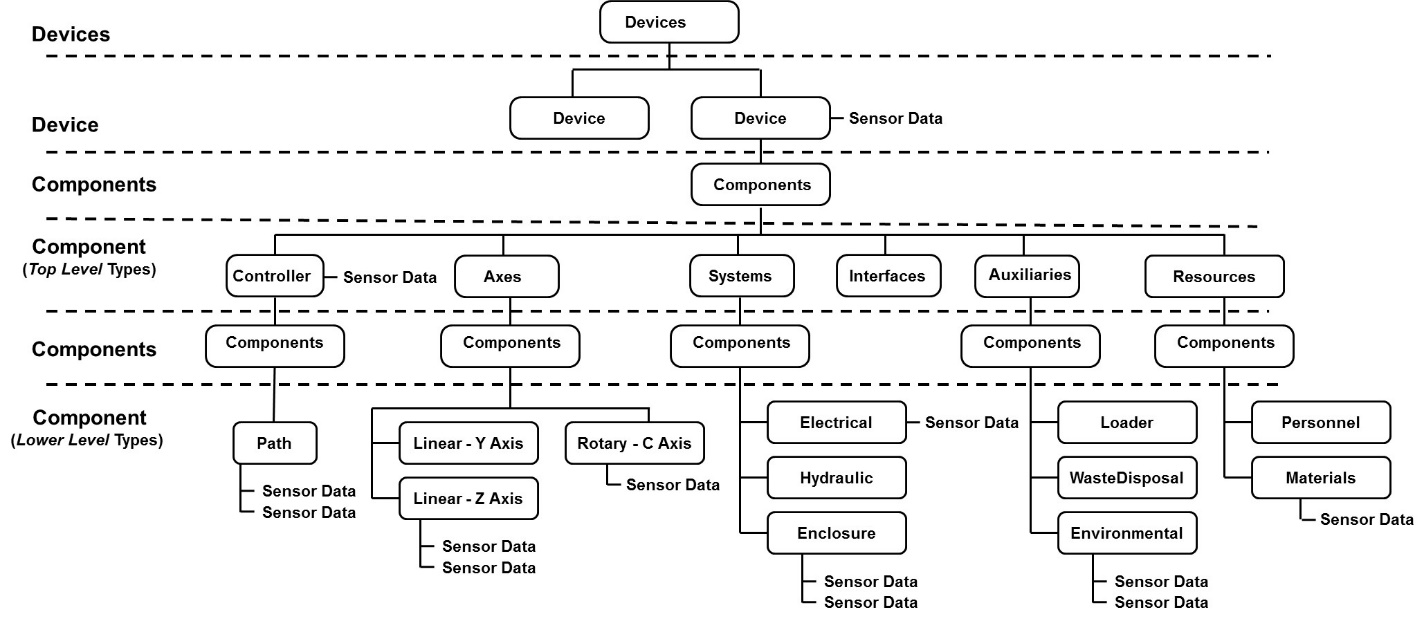
\includegraphics[width=.75\textwidth]{figures/sensor-data-associations.png}
  \caption{Sensor Data Associations}
  \label{fig:sensor-data-associations}
\end{figure}

\subsection{Sensor Unit}
\label{sec:Sensor Unit}

A \gls{sensor unit} is an intelligent piece of equipment that manages the functions of one or more \glspl{sensing element}.

Typical functions of the \gls{sensor unit} include:

\begin{itemize}
\item convert low level signals from the \glspl{sensing element} into data that can be used by other pieces of equipment.  (Example:  Convert a non-linear millivolt signal from a temperature sensor into a scaled temperature value that can be transmitted to another piece of equipment.)

\item process \gls{sensing element} data into calculated values.  (Example:  temperature sensor data is converted into calculated values of average temperature, maximum temperature, minimum temperature, etc.)

\item provide calibration and configuration information associated with each \gls{sensing element}

\item monitor the health and integrity of the \glspl{sensing element} and the \gls{sensor unit}.  (Example:  The \gls{sensor unit} may provide diagnostics on each \gls{sensing element} (e.g., open wire detection) and itself (e.g., measure internal temperature of the \gls{sensor unit}).
\end{itemize}

Depending on how the \gls{sensor unit} is used, it may be considered as either an independent piece of equipment and modeled in the \gls{xml} document as a \gls{device}, or it may be modeled as a \gls{top level} \gls{component} called \gls{sensor} if it is integral to a piece of equipment.

A \gls{sensor} \may have its own \gls{uuid} so it can be tracked throughout its lifetime.

The following examples demonstrate how a \gls{sensor term} may be modeled in the \gls{xml} document differently based on how the \gls{sensor term} functions within the overall piece of equipment

Example\#1:   If the \gls{sensor} provides vibration measurement data for the spindle on a piece of equipment, it could be modeled as a \gls{sensor} for rotary axis named C.

\begin{lstlisting}[firstnumber=1,escapechar=|,%
    caption={Example of Sensor for rotary axis}, label={lst:example-of-sensor}]
<Components>
  <Axes
    <Components>
      <Rotary id="c" name="C">
        <Components>
          <Sensor id="spdlm" name="Spindlemonitor">
            <DataItems>
              <DataItem type="DISPLACEMENT" id="cvib"
                category="SAMPLE" name="Svib" 
                units="MILLIMETER"/>
            </DataItems>
          </Sensor >
        <Components>
      </Rotary>
    </Components>
  </Axes>
</Components>
\end{lstlisting}

Example\#2:   If a \gls{sensor} provides measurement data for multiple \gls{component} elements within a piece of equipment and is not associated with any particular \gls{component} element, it \may be modeled in the \gls{xml} document as an independent \gls{lower level} \gls{component} and the data associated with measurements are associated with their associated \gls{component} elements.

This example represents a \gls{sensor unit} with two \glspl{sensing element}, one measures spindle vibration and the other measures the temperature for the X axis.   The \gls{sensor unit} also has a \gls{sensing element} measuring the internal temperature of the \gls{sensor unit}.

\begin{lstlisting}[firstnumber=1,escapechar=|,%
    caption={Example of Sensor Unit with Sensing Element}, label={lst:example-of-sensor-with-sensing-elements}]
<Device id="d1" uuid="HM1" name="HMC_3Axis">
  <Description>3 Axis Mill</Description>
  <Components>
    <Axes
      <Components>
        <Sensor id="sens1" name="Sensorunit">
          <DataItems>
            <DataItem type="TEMPERATURE" id="sentemp"
              category="SAMPLE" name="Sensortemp" 
              units="DEGREE"/> 
          </DataItems>
        </Sensor >
        <Rotary id="c" name="C">
          <DataItems>
            <DataItem type="DISPLACEMENT" id="cvib"
              %category="SAMPLE" name="Svib" 
              units="MILLIMETER">
                <Source componentId="sens1"/>
            <DataItem/>
          </DataItems>
        </Rotary>
        <Linear id="x" name="X">
          <DataItems>
            <DataItem type="TEMPERATURE" id="xt" 
              category="SAMPLE" name="Xtemp" 
              units="DEGREE">
                <Source componentId="sens1"/>
            <DataItem/>
          </DataItems>
        </Linear>
      <Components>
    </Axes>
  </Components>
</Device>
\end{lstlisting}

\subsection{Sensor Configuration}
\label{sec:Sensor Configuration}

When a \gls{sensor} unit is modeled in the \gls{xml} document as a \gls{component} or as a separate piece of equipment, it may provide additional configuration information for the \glspl{sensor element} and the \gls{sensor unit} itself.  

\gls{configuration} data provides information required for maintenance and support of the sensor.

\gls{configuration} data is only available when the \gls{sensor} unit is modeled as a \gls{component} or a separate piece of equipment. For details on the modeling of configuration data in the \gls{xml} document, see \sect{Configuration for Component}.

When \gls{sensor} represents the \gls{sensor unit} for multiple \gls{sensing element}(s), each sensing element is represented by a \gls{channel}.   The \gls{sensor unit} itself and each \gls{channel} representing one \gls{sensing element} \may have its own configuration data.

\gls{sensorconfiguration} can contain any descriptive content for a \gls{sensor unit}.  This element is defined to contain mixed content and additional \gls{xml} elements (indicated by the \gls{any} element in \fig{sensorconfiguration-schema-diagram}) \may be added to extend the schema for \gls{sensorconfiguration}.

\fig{sensorconfiguration-schema-diagram} represents the structure of the \gls{sensorconfiguration} \gls{xml} element showing the attributes defined for \gls{sensorconfiguration}. 

\begin{figure}[ht]
  \centering
  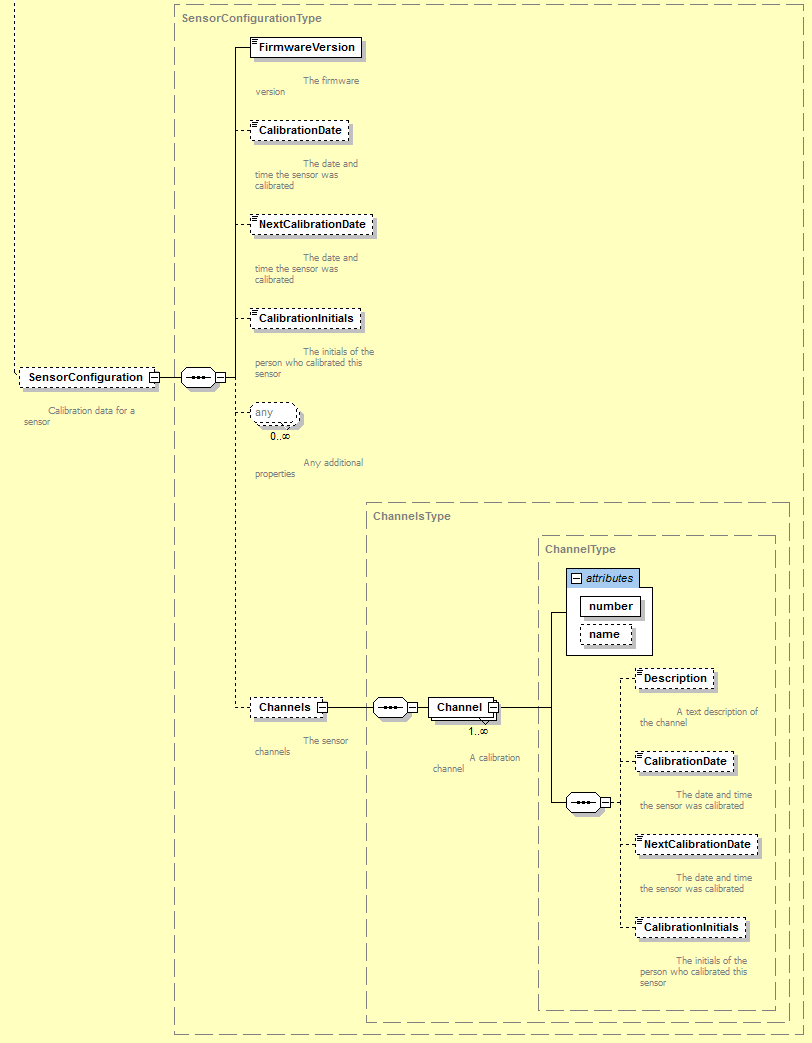
\includegraphics[width=.75\textwidth]{figures/sensorconfiguration-schema-diagram.png}
  \caption{SensorConfiguration Diagram}
  \label{fig:sensorconfiguration-schema-diagram}
\end{figure}
\FloatBarrier

\tabulinesep = 5pt
\begin{longtabu} to \textwidth {
    |l|X[3l]|X[0.75l]|}
\caption{MTConnect SensorConfiguration Element} \label{table:mtconnect-sensorconfiguration-element} \\

\hline
Element & Description & Occurrence \\
\hline
\endfirsthead

\hline
\multicolumn{3}{|c|}{Continuation of Table \ref{table:mtconnect-sensorconfiguration-element}}\\
\hline
Element & Description & Occurrence \\
\hline
\endhead
 
\gls{sensorconfiguration}
&
An element that can contain descriptive content defining the configuration information for \gls{sensor}.
\newline For \gls{sensor}, the valid configuration is \gls{sensorconfiguration} which provides data from a subset of items commonly found in a transducer electronic data sheet for sensors and actuators called
TEDS.
\newline TEDS formats are defined in IEEE 1451.0 and 1451.4 transducer interface standards (ref 15 and 16, respectively).
\newline MTConnect does not support all of the data represented in the TEDS data, nor does it duplicate the function of the TEDS data sheets. 
&
0..1 \\
\hline


\end{longtabu}


\subsubsection{Elements for SensorConfiguration}

\tbl{elements-for-sensorconfiguration} defines the configuration elements available for \gls{sensorconfiguration}:

\tabulinesep = 5pt
\begin{longtabu} to \textwidth {
    |l|X[3l]|X[0.75l]|}
\caption{Elements for SensorConfiguration} \label{table:elements-for-sensorconfiguration} \\

\hline
Element & Description & Occurrence \\
\hline
\endfirsthead

\hline
\multicolumn{3}{|c|}{Continuation of Table \ref{table:elements-for-sensorconfiguration}}\\
\hline
Element & Description & Occurrence \\
\hline
\endhead

\gls{firmwareversion}
&
\glsentrydesc{firmwareversion}
\newline \gls{firmwareversion} is a required element if \gls{sensorconfiguration} is used.
\newline The data value for \gls{firmwareversion} is provided in the \gls{cdata} for this element and \MAY be any numeric or text
content.
&
1 \\
\hline

\gls{calibrationdate}
&
Date upon which the \gls{sensor unit} was last calibrated.
\newline The data value for \gls{calibrationdate} is provided in the \gls{cdata} for this element and \MUST be represented in the W3C ISO 8601 format.
&
0..1 \\
\hline

\gls{nextcalibrationdate}
&
Date upon which the \gls{sensor unit} is next scheduled to be calibrated.
\newline The data value for \gls{nextcalibrationdate} is provided in the \gls{cdata} for this element and \MUST be represented in the W3C ISO 8601 format.
&
0..1 \\
\hline

\gls{calibrationinitials}
&
\glsentrydesc{calibrationinitials}
\newline The data value for \gls{calibrationinitials} is provided in the \gls{cdata} for this element and \MAY be any numeric or text
content.
&
0..1 \\
\hline

\gls{channels}
&
\glsentrydesc{channels}
&
0..1 \\
\hline

\end{longtabu}

\paragraph{Attributes for Channel}\mbox{}

\gls{channel} represents each \gls{sensing element} connected to a \gls{sensor unit}. \tbl{attributes-for-channel} defines the attributes for \gls{channel}:

\tabulinesep = 5pt
\begin{longtabu} to \textwidth {
    |l|X[3l]|X[0.75l]|}
\caption{Attributes for  Channel} \label{table:attributes-for-channel} \\

\hline
Attribute & Description & Occurrence \\
\hline
\endfirsthead

\hline
\multicolumn{3}{|c|}{Continuation of Table \ref{table:attributes-for-channel}}\\
\hline
Attribute & Description & Occurrence \\
\hline
\endhead
 
\gls{number} 
&
A unique identifier that will only refer to a specific \gls{sensing element}.
\newline \gls{number} is a required attribute.
\newline For example, this can be the manufacturer code and the serial number.
\newline \gls{number} \SHOULD be alphanumeric and not exceeding 255
characters.
\newline An \gls{nmtoken} XML type.
&
1 \\
\hline

\gls{name}
&
The \gls{name} of the \gls{sensing element}.
\newline \gls{name} is an optional attribute.
\newline \gls{name} \SHOULD be unique within the \gls{sensor unit} to allow for easier data integration. 
\newline An \gls{nmtoken} XML type.
&
0..1 \\
\hline

\end{longtabu}

\paragraph{Elements for Channel}\mbox{}

\tbl{elements-for-channel} describes the elements provided for \gls{channel}.

\tabulinesep = 5pt
\begin{longtabu} to \textwidth {
    |l|X[3l]|X[0.75l]|}
\caption{Elements for Channel} \label{table:elements-for-channel} \\

\hline
Element & Description & Occurrence \\
\hline
\endfirsthead

\hline
\multicolumn{3}{|c|}{Continuation of Table \ref{table:elements-for-channel}}\\
\hline
Element & Description & Occurrence \\
\hline
\endhead

\gls{description}
&
An XML element that can contain any descriptive content.
\newline The \gls{cdata} of \gls{description} \MAY include any additional descriptive information the implementer chooses to include regarding a \gls{sensor element}.

&
0..1 \\
\hline

\gls{calibrationdate}
&
Date upon which the \gls{sensor unit} was last calibrated to the \gls{sensor element}.
\newline The data value for \gls{calibrationdate} is provided in the \gls{cdata} for this element and \MUST be represented in the W3C ISO 8601 format.
&
0..1 \\
\hline

\gls{nextcalibrationdate}
&
Date upon which the \gls{sensor element} is next scheduled to be calibrated with the \gls{sensor unit}.
\newline The data value for \gls{nextcalibrationdate} is provided in the \gls{cdata} for this element and \MUST be represented in the W3C ISO 8601 format.
&
0..1 \\
\hline

\gls{calibrationinitials}
&
\glsentrydesc{calibrationinitials}
\newline The data value for \gls{calibrationinitials} is provided in the \gls{cdata} for this element and \MAY be any numeric or text content.
&
0..1 \\
\hline

\end{longtabu}

\lst{example-of-sensor-configuration-data} is an example of the configuration data for \gls{sensor} that is modeled as a \gls{component}.  It has \gls{configuration} data for the \gls{sensor unit}, one \gls{channel} named A/D:1, and two \gls{dataitems} – \glselementname{voltage sample} (as a \gls{sample category}) and \glselementname{voltage sample} (as a \gls{condition category} or alarm).

\begin{lstlisting}[firstnumber=1,escapechar=|,%
    caption={Example of configuration data for Sensor}, label={lst:example-of-sensor-configuration-data}]
<Sensor id="sensor" name="sensor">
  <Configuration>
    <SensorConfiguration>
      <FirmwareVersion>2.02</FirmwareVersion>
      <CalibrationDate>2010-05-16</CalibrationDate>
      <NextCalibrationDate>2010-05-16</NextCalibrationDate>
      <CalibrationInitials>WS</CalibrationInitials>
      <Channels>
        <Channel number="1" name="A/D:1">
          <Description>A/D With Thermister</Description>
        </Channel>
      </Channels>
    </SensorConfiguration>
  </Configuration>
  <DataItems>
    <DataItem category="CONDITION" id="senvc" 
      type="VOLTAGE" />
    <DataItem category="SAMPLE" id="senv" 
      type="VOLTAGE" units="VOLT" subType="DIRECT" />
  </DataItems>
</Sensor>
\end{lstlisting}


